% mnras_template.tex 
%
% LaTeX template for creating an MNRAS paper
%
% v3.0 released 14 May 2015
% (version numbers match those of mnras.cls)
%
% Copyright (C) Royal Astronomical Society 2015
% Authors:
% Keith T. Smith (Royal Astronomical Society)

% Change log
%
% v3.0 May 2015
%    Renamed to match the new package name
%    Version number matches mnras.cls
%    A few minor tweaks to wording
% v1.0 September 2013
%    Beta testing only - never publicly released
%    First version: a simple (ish) template for creating an MNRAS paper

%%%%%%%%%%%%%%%%%%%%%%%%%%%%%%%%%%%%%%%%%%%%%%%%%%
% Basic setup. Most papers should leave these options alone.
\documentclass[fleqn,usenatbib]{mnras}

% MNRAS is set in Times font. If you don't have this installed (most LaTeX
% installations will be fine) or prefer the old Computer Modern fonts, comment
% out the following line
\usepackage{newtxtext,newtxmath}
% Depending on your LaTeX fonts installation, you might get better results with one of these:
%\usepackage{mathptmx}
%\usepackage{txfonts}

% Use vector fonts, so it zooms properly in on-screen viewing software
% Don't change these lines unless you know what you are doing
\usepackage[T1]{fontenc}

% Allow "Thomas van Noord" and "Simon de Laguarde" and alike to be sorted by "N" and "L" etc. in the bibliography.
% Write the name in the bibliography as "\VAN{Noord}{Van}{van} Noord, Thomas"
\DeclareRobustCommand{\VAN}[3]{#2}
\let\VANthebibliography\thebibliography
\def\thebibliography{\DeclareRobustCommand{\VAN}[3]{##3}\VANthebibliography}


%%%%% AUTHORS - PLACE YOUR OWN PACKAGES HERE %%%%%

% Only include extra packages if you really need them. Common packages are:
\usepackage{graphicx}	% Including figure files
\usepackage{amsmath}	% Advanced maths commands
% \usepackage{amssymb}	% Extra maths symbols

%%%%%%%%%%%%%%%%%%%%%%%%%%%%%%%%%%%%%%%%%%%%%%%%%%

%%%%% AUTHORS - PLACE YOUR OWN COMMANDS HERE %%%%%

% Please keep new commands to a minimum, and use \newcommand not \def to avoid
% overwriting existing commands. Example:
%\newcommand{\pcm}{\,cm$^{-2}$}	% per cm-squared

%%%%%%%%%%%%%%%%%%%%%%%%%%%%%%%%%%%%%%%%%%%%%%%%%%

%%%%%%%%%%%%%%%%%%% TITLE PAGE %%%%%%%%%%%%%%%%%%%

% Title of the paper, and the short title which is used in the headers.
% Keep the title short and informative.
\title[New high-ionization planetary nebula]{Discovery of a new high-ionization planetary nebula in LAMOST}

% The list of authors, and the short list which is used in the headers.
% If you need two or more lines of authors, add an extra line using \newauthor
\author[Guti\'errez-Soto et al.]{
  L. A. Guti\'errez-Soto$^{1,2}$
  \thanks{E-mail: gsoto.angel@gmail.com}
%A. N. Other,$^{2}$
%Third Author$^{2,3}$
%and Fourth Author$^{3}$
\\
% List of institutions
$^{1}$Instituto de Astrof\'{i}sica de La Plata (CCT La Plata - CONICET - UNLP), B1900FWA, La Plata, Argentina\\
$^{2}$Departamento de Astronomia, IAG, Universidade de S\~{a}o Paulo, Rua do Mat\~{a}o, 1226, 05509-900, S\~{a}o Paulo, Brazil\\
%$^{3}$Another Department, Different Institution, Street Address, City Postal Code, Country
}

% These dates will be filled out by the publisher
\date{Accepted XXX. Received YYY; in original form ZZZ}

% Enter the current year, for the copyright statements etc.
\pubyear{2015}

% Don't change these lines
\begin{document}
\label{firstpage}
\pagerange{\pageref{firstpage}--\pageref{lastpage}}
\maketitle

% Abstract of the paper
\begin{abstract}
  We report the identification of a new planetary nebula found in the catalog of
  emission line objects created by \citet{Skoda:2020} based in LAMOST data, using
  color-color diagrams based in GAIA and Pan-STARRS1 photometry. The optical LAMOST
  spectrum of this source show prominent emission lines, including highly ionized
  such as He II and [Ar V] lines. The LAMOST spectra was
  modelled using the code of photoionization  {\sc cloudy}.
  Comparing the model spectra with the observed one, we found
  the best-fit {\sc cloudy} models resulting in three best model fit.
  These model spectra have obtained a effective temperature of 14$\times10^{4}$ K.
  Other parameters such as luminosity and abundances were determined by
  comparing with the model. Comparing with evolution track of post-AGB
  I found that the mass of the progenitor star is 1.25 M{$\odot$}. Bla Bla Bla Bla
  Bla Bla Bla Bla Bla Bla Bla Bla Bla
\end{abstract}

% Select between one and six entries from the list of approved keywords.
% Don't make up new ones.
\begin{keywords}
planetary nebulae: general -- ISM: lines and bands -- surveys
\end{keywords}

%%%%%%%%%%%%%%%%%%%%%%%%%%%%%%%%%%%%%%%%%%%%%%%%%%

%%%%%%%%%%%%%%%%% BODY OF PAPER %%%%%%%%%%%%%%%%%%

\section{Introduction}

\label{sec:intro}

Planetary nebulae (PNe) are gaseous layers and dust, representing the last stage of
evolution of low- and intermediate-mass stars (0.8$\msol$ - 8.0$\msol$).
The PNe phase begin when gas is ejected from the red giant stars late phase of
their lives. Subsequently this gas is ionized by the radiation field coming from the remnant
star resulted. An emission nebula expands, a glowing shell of ionized gas until lost in the
interstellar medium. Then the dying star core becomes a white dwarf.

The number of these kind of objects discovered in the galaxy is relatively low (\(\sim 3,500\)).
However, this current number of PNe identify on the Milky Way is far away (which represents
only about 15-30\%) of the estimated total of Galactic PNe (\citealp{Frew:2008}; \citealp{Jacoby:2010})
showing that a small fraction of the PNe have been cataloged until now \citep{Frew:2017}.
If this is true, there will be a much larger number of PNe in the Galaxy waiting to be discovery.
The models of \citet{Moe:2006}, for example, predict that there are 46,000 $\pm$ 22,000
for the general case, but only $\sim$6600 \citep{Marco:2005} if close binaries
(e.g. common-envelope phase) are required. \citet{Miszalski:2009} confirm earlier estimates
that the binary fraction of PN central stars is only 10-20\% of all
PNe, and thus, binarity is not likely to be a major factor in
the formation process. This mean that the search for planetary nebulae
becoming a important task, that eavery time is more dificult, due to that many of
the undiscovered PNe are probably the more distant and then the weakest.
And because many of them, probably, are located in nuvens of dust.
And note that planetary nebulae only last for about 5,000-25,000 yr \citep{Badenes:2015},
making them a very short-lived part of the stellar life cycle.
But why is it import to discovery new planetary nebula? the answer could be very obvious and is
related with the idea that PNe provide vital clues for the understanding late-stage stellar
evolution and Galactic chemical enrichment. Their strong emission lines allow the determination
of abundances, expansion and radial velocities, and
CSPN temperatures. The PN phase enriches the ISM with nitrogen, carbon, helium,
and dust, important components in the formation of future
generations of stars. PNe yield information on the nuclear
burning, dredge up, and mass loss in the stellar progenitor
(see \citealp{Kwitter:2022} for an excellent recent PN
review). Thus, we need to know the number of PNe in
the Galaxy in order to develop accurate models of 
chemical enrichment rates since the Galaxy was young.

PN studies have been hampered by three problems:
(i) the previous lack of accurate distances to most Galactic
PNe; (ii) obtaining representative PNe samples of the true
population diversity \citep{Parker:2022}, and (iii) their unknown
progenitor masses. The first problem tend to be
resolved via accurate Gaia CSPN distances, though many
CSPNe remain too distant and faint for Gaia DR3 and correct
CSPN identification continues being a problem \citep{Parker:2022}.
The second problem is being addressed by deep, narrow-band,
wide-field surveys, e.g., \citet{Parker:2005},
\citet{Drew:2005}, and \citet{Drew:2014}. For the third problem
of progenitor masses, these can only be accurately determined for
PNe in Galactic globular and open clusters (OCs). These allow precise
distance determinations from color-magnitude diagrams (CMD) and Gaia
\citep{Fragkou:2022}. Then, these problems could be addressed by increasing the
number of PNe in the Galaxy, because a better study and statistical
could been done. For this reason, several attempted have been performed
in the past based diagnostic diagrams using several emission-line
intensities to differentiate resolved emission
sources such as PN from H {\sc ii} regions, SNRs and other objects.
Diagnostic diagram based on the H{$\alpha$}/[N II] and H{$\alpha$}/[S II]
emission-line ratios \citep{Sabbadin:1977, Fesen:1985, Riesgo:2006}.
The selection criteria were empirically derived in theses diagrams,
by using emission lines ratios observed in PNe, supernova remnants, and H{\sc ii}
regions. \citet{Viironen:2009a, Viironen:2009b} used two color-color diagrams
based on IPHAS and 2MASS photometry to discriminate PNe from stellar and other
emission lines sources in the Galactic context. The methodology more used to
identify compact PNe consists in the identification of candidate in narrow- and
broad-band photometric surveys and reveler their true nature through follow-up
spectroscopic. This always is required with such samples because the success
of finding compact PNe with photometric diagrams is low, being dominated for
other type of compact emitters.

Recently, \citet{Akras:2019b} using the classification tree model
found new colour criteria to identify compact PNe by
using both 2MASS and AllWISE photometric data. \citet{Gutierrez-Soto:2020}
searched for compact PNe in the Javalambre and Southern Photometric Local
Universe Survey data (J-PLUS and S-PLUS, respectively), using a combination
of narrow- and broad-band photometry. And new diagnostic diagram were proposed
by \citet{Vejar:2019} to find for new PNe using broad-band filters.
In this order of ideas, in an attempts to create new color-color criteria based
in larges photometric surveys: GAIA and Pan-STARRS. We found a color criteria
based on theses surveys, on which PNe with strong H{$\alpha$} are puts in
evidence. We applied this criteria to the sample of emission lines of \citet{Skoda:2020}
constructed using the LAMOST DR? data. The strong emission lines of our target can
be easily identified in the low-resolution spectrum (R$\sim$1,800), which covers
the full optical range from 3,700 to 9,000 \AA.

In this manuscript is presented a possible new planetary nebula based in
its LAMOST spectra, which displays strong nebular emission lines, including high-ionizing
line increasing the chance of the object will be a real PN.
At the moment of this manuscript was written we noted that the
object now appears classified as galaxy in SIMBAD, but our analysis
suggested that the source is in reality an high-excitation PN. 
Section~\ref{sec:metho} describes the observations related to the GAIA,
Pans-STARR and LAMOST. It also presents the technique implemented 
to select the PN candidate. In Section~\ref{sec:comp} is presented
a comparison between the new PN identified with other ionization known PNe
to validate the new find. Section~\ref{sec:model} describes the modelled {\sc cloudy}
of the PN candidate. In Section~\ref{sec:tracks}, we compare the modelled spectra of
observed one with post-AGB stellar evolution track, and finally
Section~\ref{sec:conclu} discusses our main results and conclusions.

\section{Finding a new possible PN}
\label{sec:metho}

In order to bring to the reader a small overview of the data used
in this manuscript, we present in a few words the three
surveys basis of this work.

\subsection{GAIA EDR3}
\label{sec:gaia}

The early installment of the third GAIA data release (EDR3; \citealp{Brown:2021})
was made available to the public on 2020 December, which contain which contains
the first 34 months of data collection of the Gaia mission \citep{Brown:2018}.
It consist of around 1.8 billion sources with precise astrometry as well as
photometry in the $G$, $G_{BP}$ and $G_{RP}$ bands. Gaia EDR3 made
significant improvements in precision and accuracy of
photometric magnitudes, parallax, celestial positions, and proper
motions with respect to Gaia DR2. This means that it improved
the efficiency of candidate selection of a variety of
objects, for instance, recently,  \citet{Christy:2023} used features
derived from GAIA photometry and other surveys to identify new variable stars.
Note that recently, GAIA (more specify GAIA DR2) have been implemented
to search for central stars of planetary nebulae \citep{Chornay:2020}.

\subsection{Pan-STARRS DR1}
\label{sec:PS1}

Pan-STARRS1 (PS1; \citealp{Kaiser:2010}) is a multi-wavelength, multi-epoch,
optical imaging survey which covers $\approx$75\% of the sky. PS1 goes $\sim$1 mag
fainter than SDSS in the $z$-band \citep{York:2000}. The survey’s five optical
filters, $g$P1, $r$P1, $i$P1, $z$P1, and $y$P1, are described in
\citet{Stubbs:2010} and \citet{Tonry:2012}. At each epoch a single field
is exposed for 60s in $g$P1, 38s in $r$P1, and 30s in $i$P1, $z$P1,
and $y$P1. The photometry and astrometry from each epoch
have been combined to obtain average magnitudes and proper
motions. New central stars are been identified via
eep archival Pan-STARRS broad-band imagery \citep{Tan:2023}. 

\subsection{LAMOST}
\label{sec:lamost}

The Large Sky Area Multi-Object Fiber Spectroscopic Telescope
(LAMOST, also named Guoshoujing Telescope) is 4 m quasi-meridian reflecting
Schmidt telescope dedicated for spectroscopic sky survey.
There are 4000 fibers within a diameter of 1.75 meters (corresponding
to 5$^{\circ}$ in the sky) at the focal surface \citep{Cui:2012}, LAMOST can
obtain 4000 spectra in one exposure.
The Low-Resolution Spectroscopic Survey (LRS) of LAMOST
began in October 2011, with a spectral resolving power ($R = \lambda/\Delta\lambda$)
of about 1800 and a wavelength coverage of
3700-9100~\AA~\citep{Zhao:2012}. The first year observation was
for the pilot survey \citep{Luo:2012, Zhao:2012},
and the regular survey began in September 2012. And since then
a larger amount  spectroscopic data are been produced for
scientific propose. Each spectrum is spliced into the blue part and the red part.
And then recorded on red and blue cameras, respectively.
The blue channel is optimized for 3700 - 5900  \AA, and the red channel for
5700 - 9000  \AA, with 200 \AA overlaps between the two channels \citep{Yao:2019}.
The integration time is 600, 1500, or 1800s. The massive spectral
database obtained by LAMOST is a rich resource for us to identify
different kinds of stars, for instance CV \citep{Sun:2021}. And given
its spectroscopy nature LAMOST give an opportunity to confirmation and, then,
reveal the true nature of objects on which its nature
can no be reveal with photometry only.

\subsection{The find}
\label{sec:find}

Many of broad-band surveys are covering a extensive area of the sky, that
are covered by those narrow-band filters. It is the case of GAIA and Pans-STARRS, which
are mapped a great are of the sky.
This means, that many of emission lines could be observed for the broad-band
survey and not for the narrow ones. Then, we thought that creating color-color
diagram to select for these objects
could give us an a opportunity for find new emission line objects, in particular PNe.
At the beginning the idea was to identify for new planetary nebula in GAIA, only.
I started to constructed possibles color-color diagrams to separate PNe from
other emission lines objects and stars using GAIA only. The separation was not
good because PNe, normal stars and other emission line stars like CVs occupy the
same region in the diagram. Then, We moved to Pan-STARRS and combining the two
surveys; Pan-STARRS1 and GAIA EDR3, was found a color-color diagram that isolate the PNe
with, strong \ha{} emission line. By using the \((G - r)\) versus \((G_{BP} - G_{RP})\)
color-color is possible to separate those PNe with excess in the $r$-broad-band
filter as is possible to see in the Fig~\ref{fig:gaia-ps}. This plot include PNe
with their corresponding central star identification in GAIA collected by \citet{Gonzalez:2021}, 
cataclysm variables \citep{Downes:2006}, supernova remnants \citep{Green:2019}, symbiotic starts
from \citet{Akras:2019a}.  
Fig~\ref{fig:gaia-ps} shows that the many of the PNe have value in
the color \(G - r\) = 0, however several PNe cover the interval in this
same color between 0 and 8, and span between -1 and 5.
The orange contours represent other emission line objects that includes CV, SySt,
YSOs, AeBe stars and SNRs. The contours becoming white at the outside indicating
that the number of objects decrease significantly. And the blue contours signify
stars from \citet{Smart:2021}. Where they occupy the region with \((G - r)\) = 0.

\begin{figure}
\centering
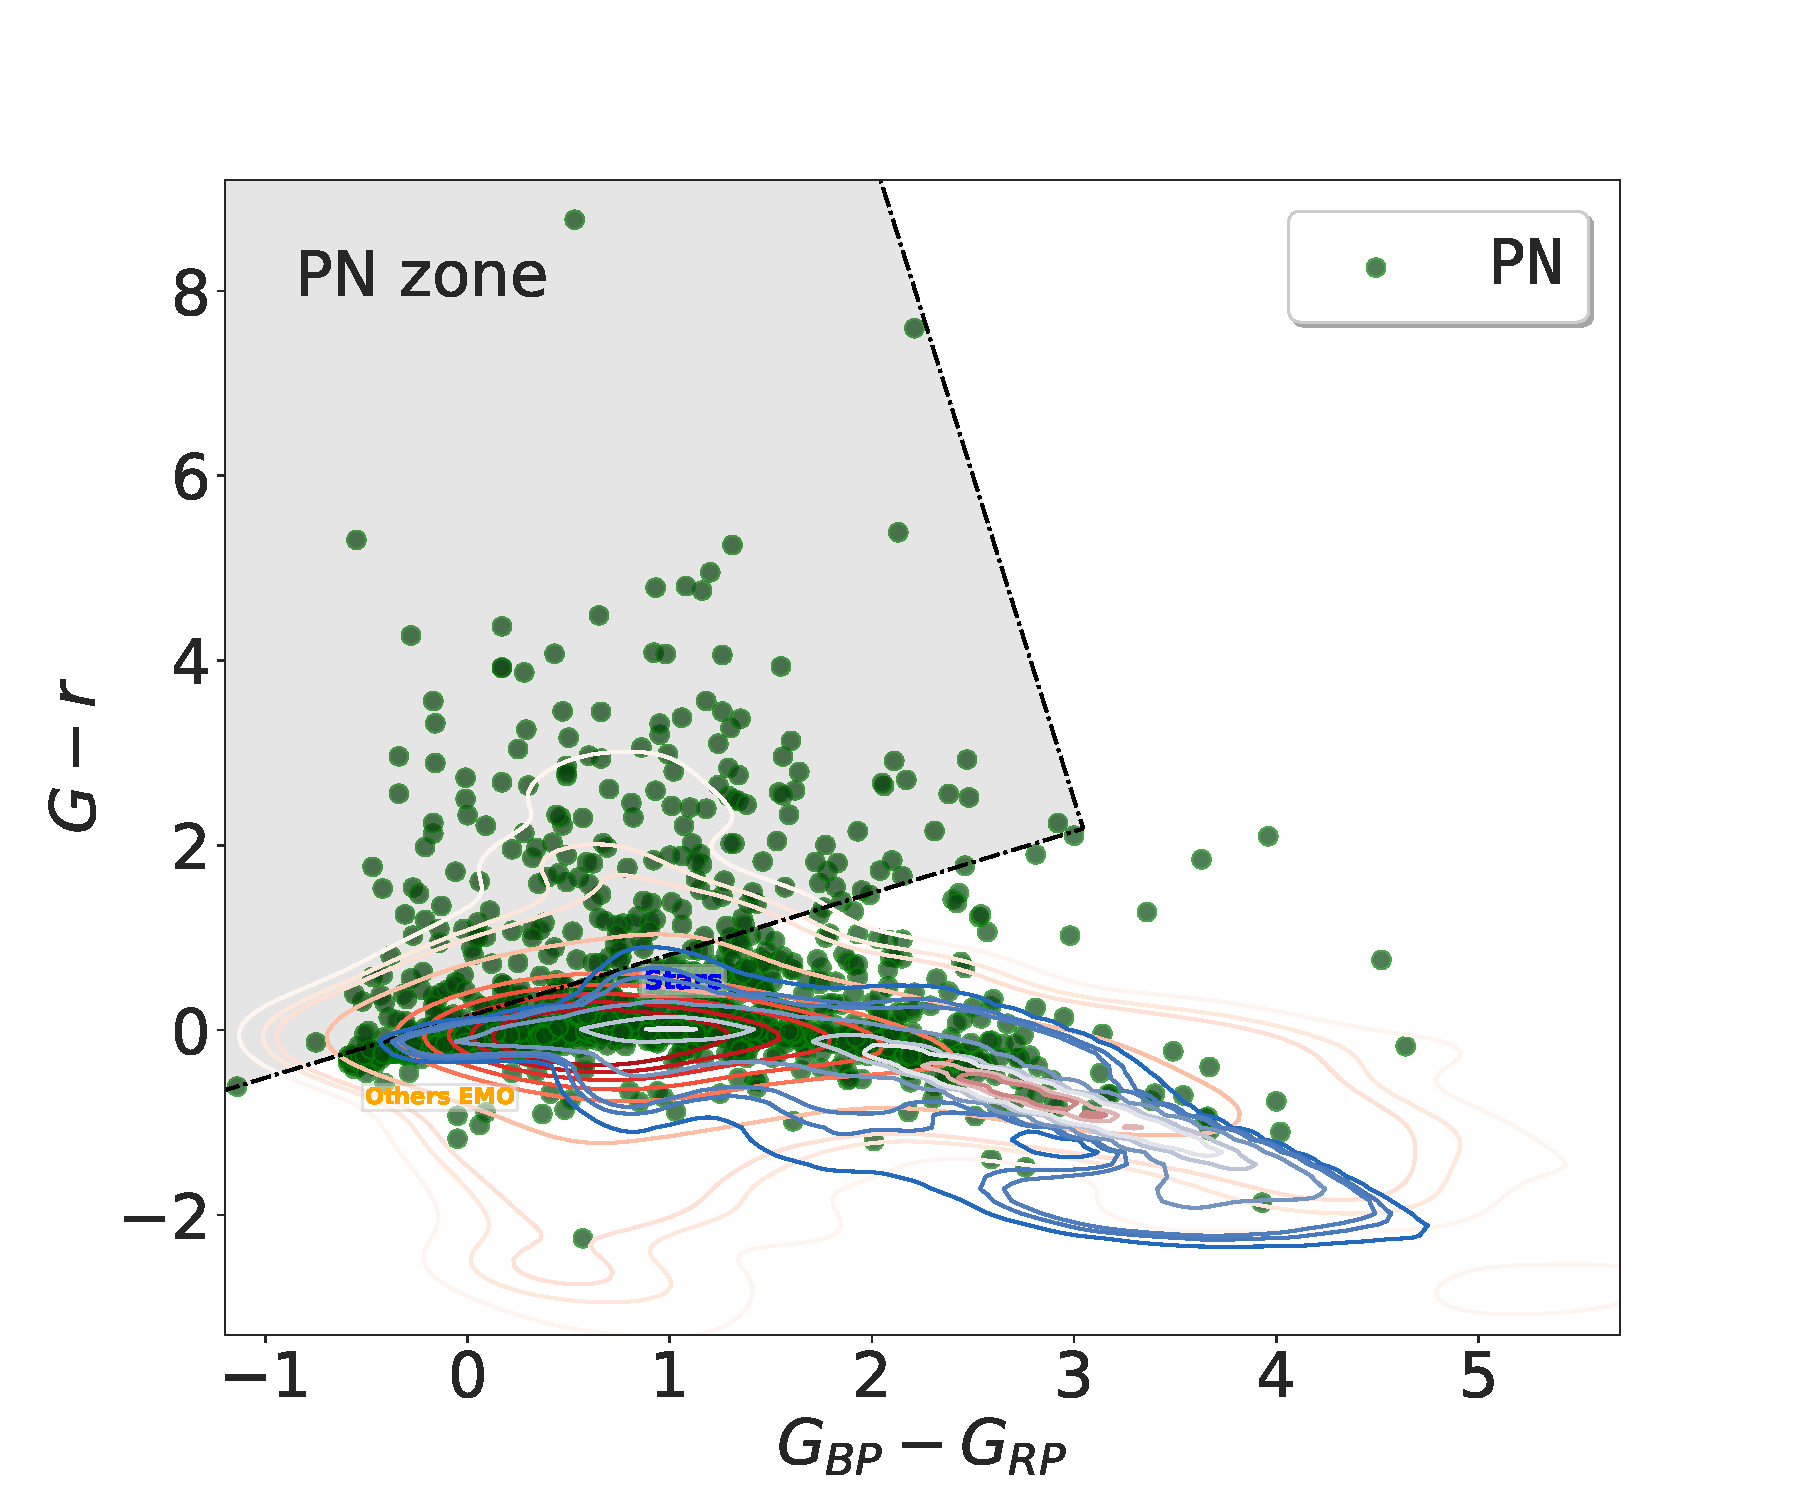
\includegraphics[width=0.9\linewidth]{Figs/color-diagram-ps-gaiaEDR3.pdf}
  \caption{} 
  \label{fig:gaia-ps}
\end{figure}

All indicate that the PNe with strong \ha{} can be selected with this color
criteria. {\sc What indicate the $G$-magnitude?.}
Then, to see the possibility of using this color criterion to select these PNe, by
testing and using the emission line catalog from \citet{Skoda:2020}. First, they
identify emission line objects from LAMOST DR4 implementing an active learning approach.
Then, they divided their final sample of emission line objects in tree subgroups.
Those with \texttt{SIMBAD} coincidences, those that are listed by \citet{Hou:2016}
and another list that are neither cross-matched with
SIMBAD nor listed by \citet{Hou:2016}. To texting the possibility to find
for new PNe with the color criteria explained above, we applied it directly in the new list,
which present objects not reported previously in the literature, which is a list with
1000 objects.

\begin{figure}
\centering
  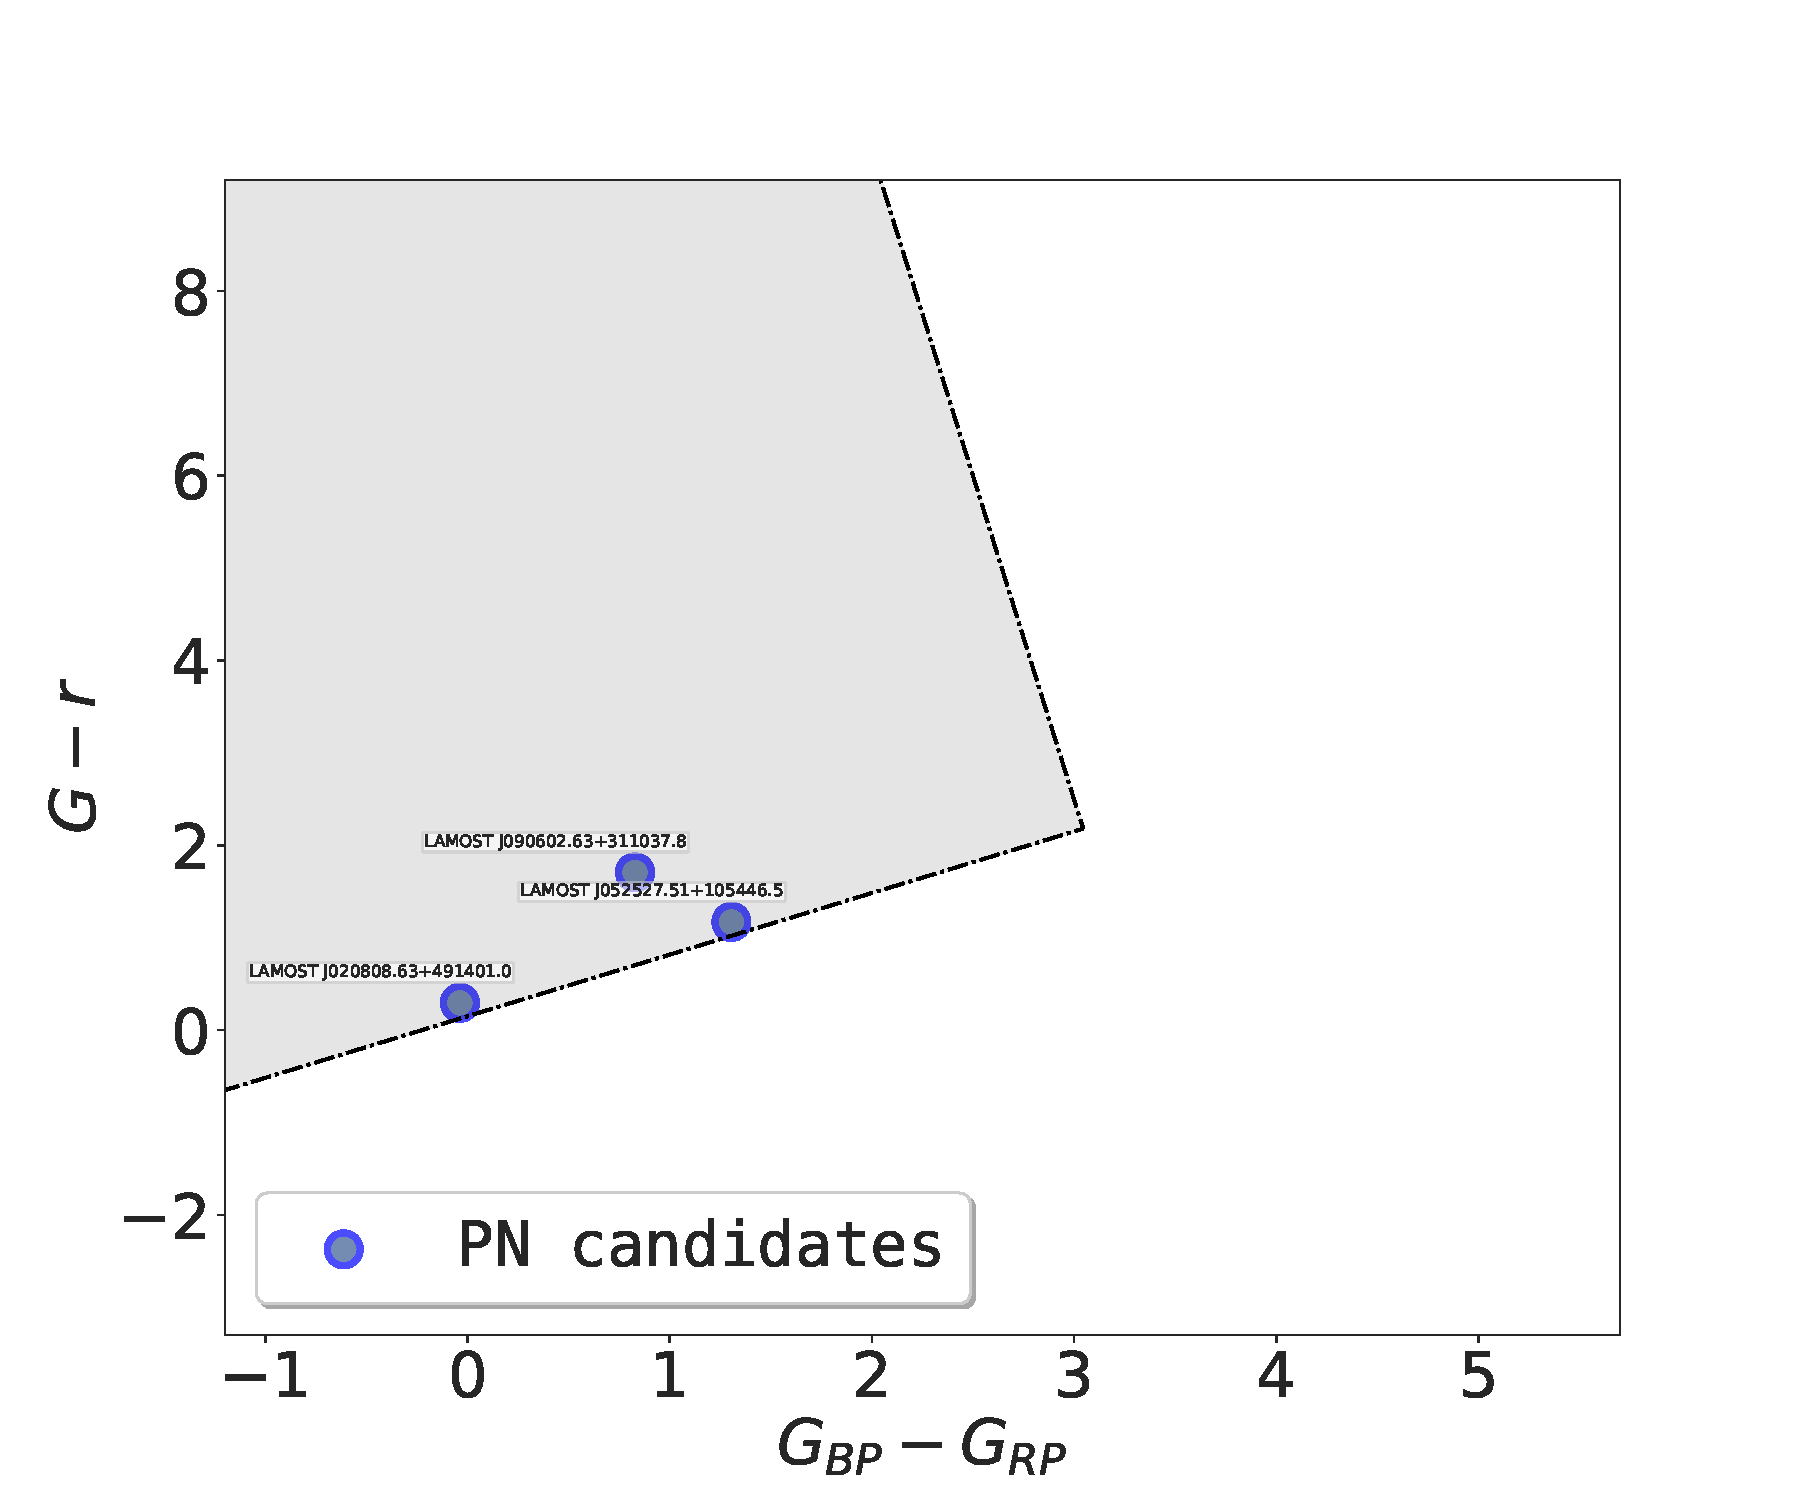
\includegraphics[width=0.9\linewidth]{Figs/pn-candidates-gaiaDR3.pdf}
  \caption{} 
  \label{fig:gaia-ps-apply}
\end{figure}

Four objects met this  condition as is possible to see in the Fig~\ref{fig:gaia-ps-apply}.
We downloaded the low resolution spectra of these objects from the LAMOST database. 
Tree objects of them display strong \ha{}, but are not display the other emission
lines typically of PNe like [O III], He II, [S II], among other. But the three look likes as PNe,
because, it displays He II emission lines, the Balmer ones, [O III], among others.

Fig~\ref{fig:spectra} shows the spectrum of the new PN finding in the list of emission
line sources of \citet{Skoda:2020}. There is an offset between the blue and red arm of
the spectrum. This probably occurs due to that the blue- and red-arm spectra were
processed separately with the 2D Pipeline and joined together after the flux calibration
\citep{Xiang:2015}. No scaling or shifting was made in cases where the blue- and
red-arm spectra did not have the same flux level in the overlapping wavelength region,
as it was unclear whether the misalignment was caused by poor flat-fielding/flux-calibration
or sky subtraction, or a combination of both \citep{Chen:2016}. That is why the spectra has
abnormal artefacts in the wavelength range 5800-6300 \AA. We have removed this part of
the spectra as possible to see in Figure~\ref{fig:spectra}, for any treatment of
this spectra. But note that no emission lines are present in this region of the spectra.
This PNe seem a very high ionization object, by eye, is possible to argue
that the He II emission line is as strong as the H$\beta$ line.
Also the presence on of [Ar V], [Ar III] and [Ne III] are indicator of being a high
ionization PN. No lines of ions in low stages of ionization were detected,
lines such as [N II] and [O II]. A preliminary analysis were performed in the next
section to try derived the physical parameters of the planetary nebula comparing
its low-resolution spectra from LAMOST with modelled 1D-spectra.

Note that the LAMOST spectra are not calibrated in absolute flux but they are
calibrate flux relative, then any analysis will have to do in term of ratio lines. 

\begin{figure*}
\centering
  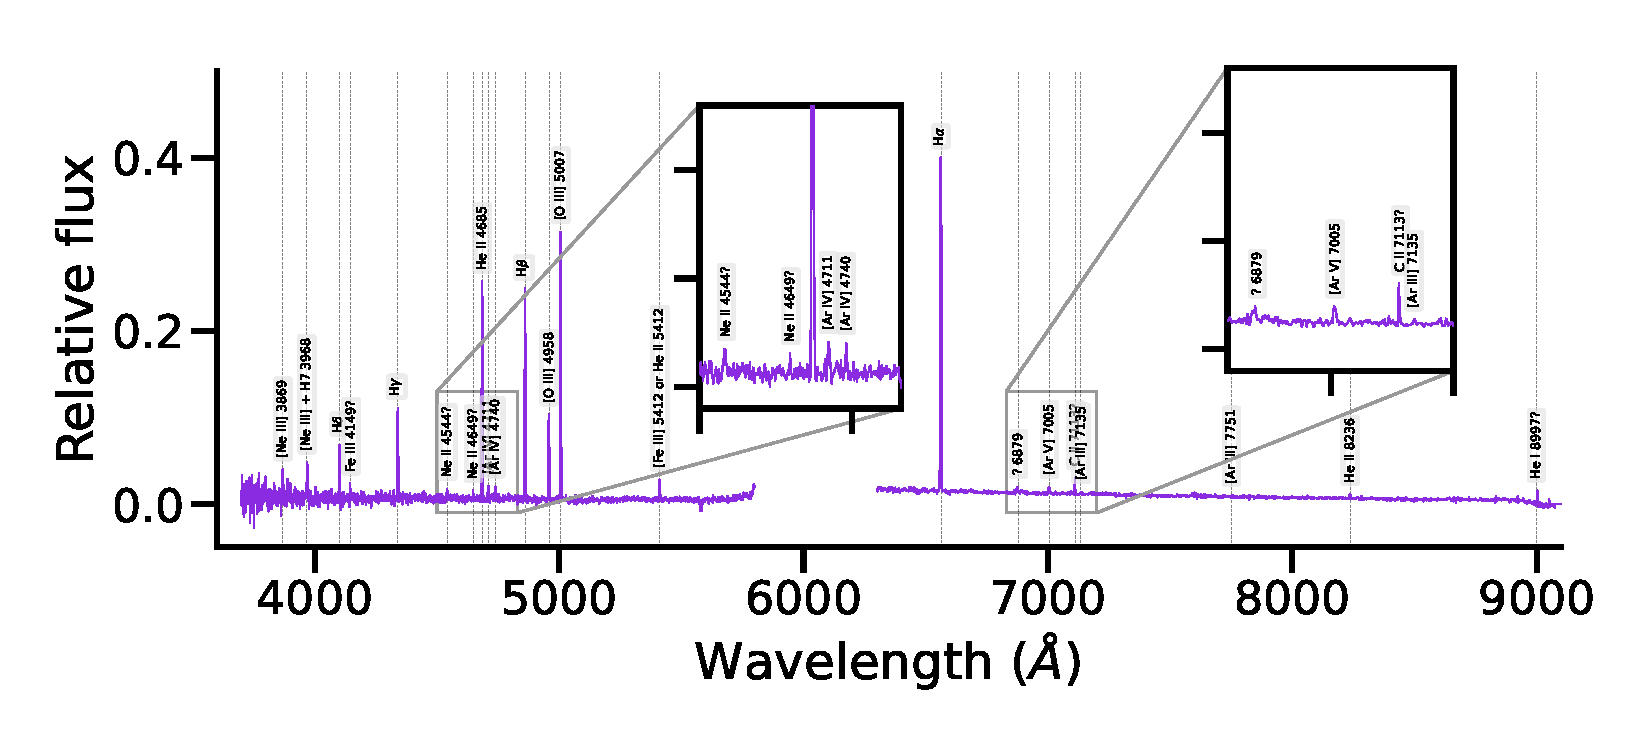
\includegraphics[width=\linewidth]{Figs/spec-56581-VB031N50V1_sp08-218.pdf}
  \caption{Low resolution spectrum from LAMOST of J020808.63+491401.0.
    The most prominent emission lines detected in the spectra are given by the dashed vertical
    lines.} 
  \label{fig:spectra}
\end{figure*}

The optical and IR-images of the PN with LAMOST
identification J020808.63+491401.0 are showed in Fig~\ref{fig:image}.
\textit{Left panel} exhibits the PanSTARRS coloured
images \footnote{These RGB images were made by implementing
the python package \texttt{aplpy} \citep{aplpy:2019}}, which
was constructed by combining the $g$, $r$ and $i$ filters in
the blue, green and red colour channels, respectively.
The image shows clearly a nebular component surrounding 
a central star. \textit{Right panel} shows the
WISE RGB image, with the filter W1, W2, and W4 in
the blue, green and red channels, respectively.
The WISE image shows that the object is W4 wright.  
At 22$\mu$ (W4-filter) it appears as an almost
circular (but slightly elongated in the north-south direction)
diffuse halo (of angular diameter of $\simeq$ 50 arcsec) surrounding
a core of bright emission centred around J020808.63+491401.0. 

\begin{figure*}
  \centering
  \begin{tabular}{l l}
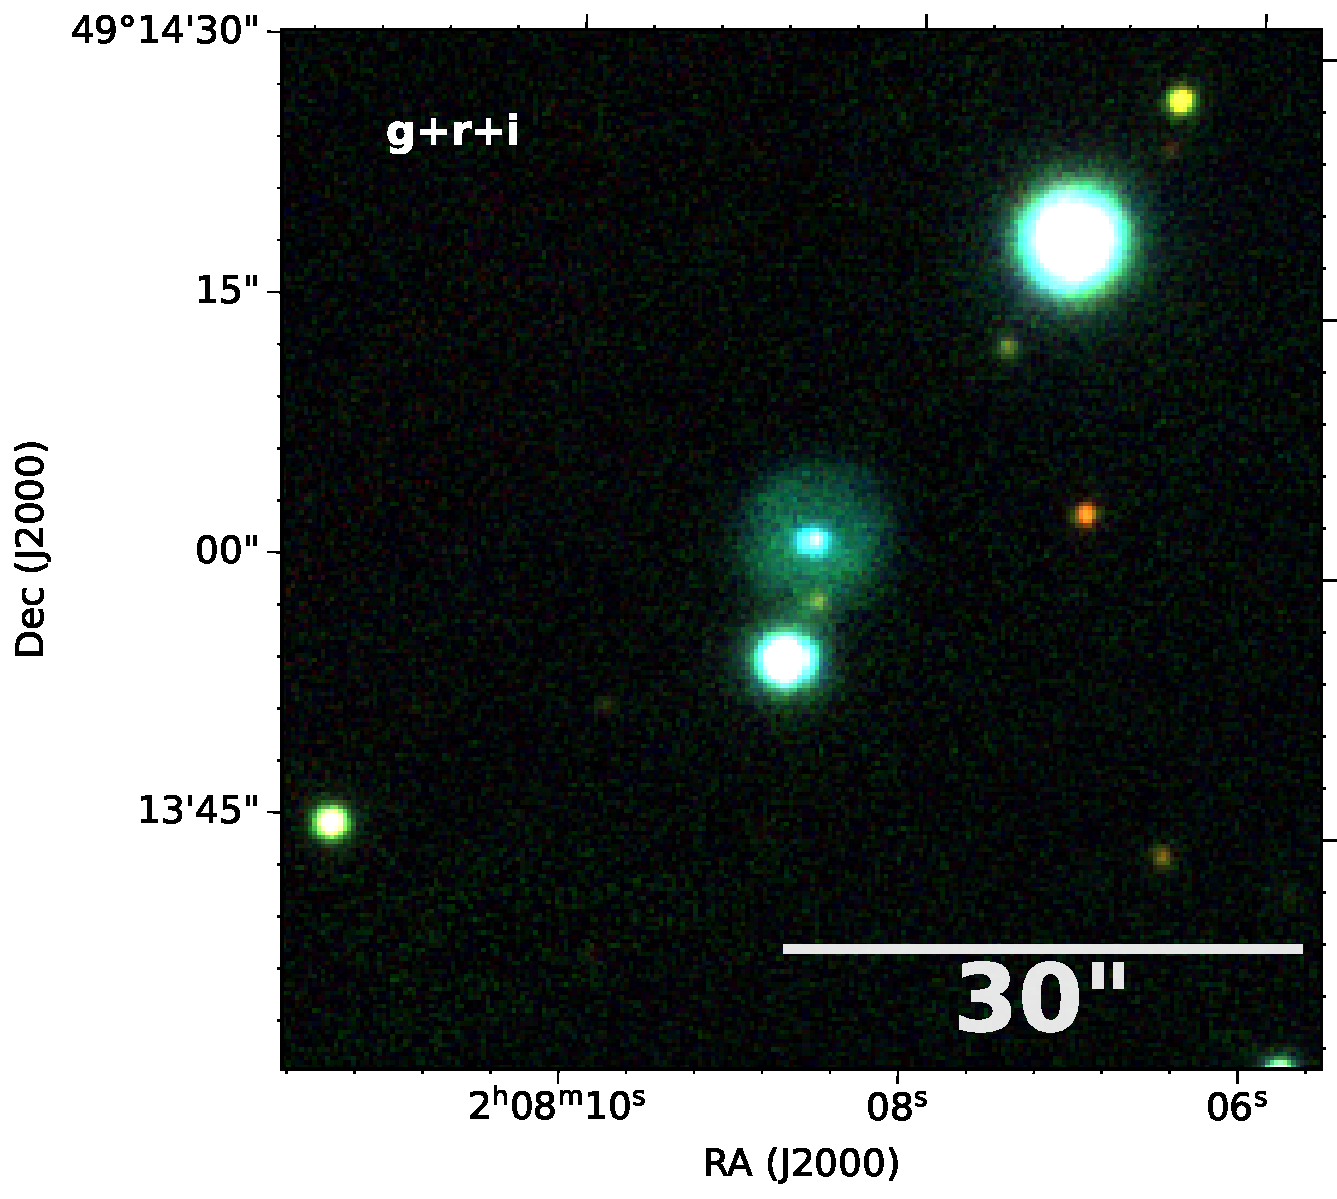
\includegraphics[width=0.5\linewidth]{Figs/cutout_rings_v3_skycell_2294_031_stk_i_unconv-irg-RGB.pdf}
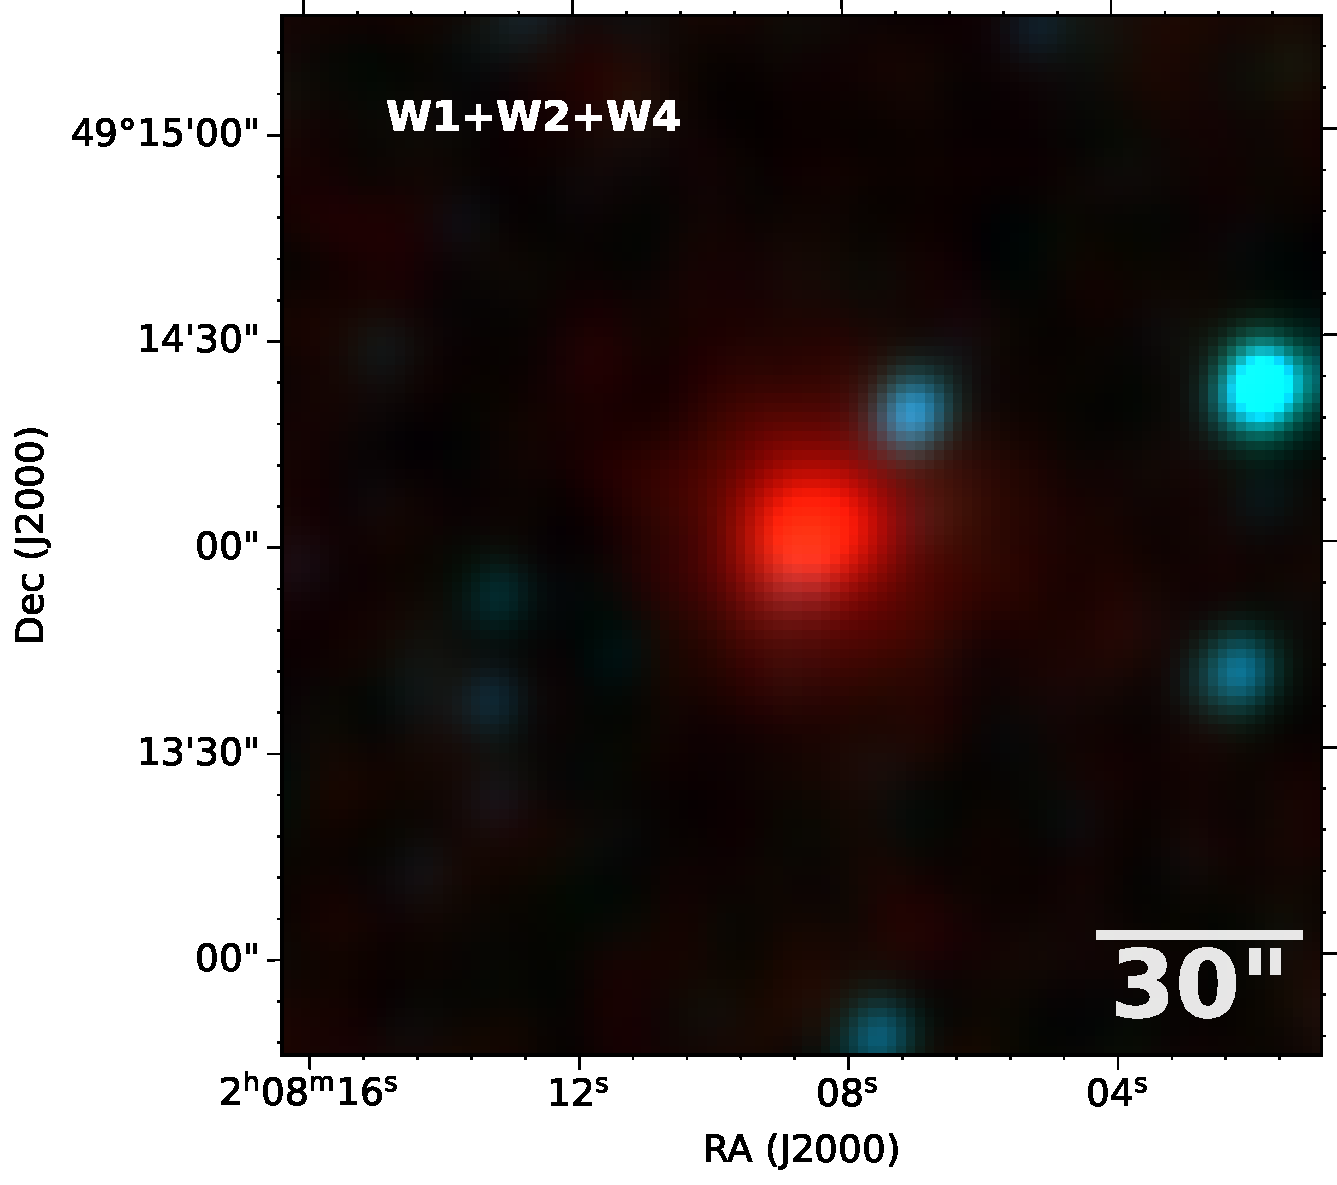
\includegraphics[width=0.5\linewidth]{Figs/w4_ra32_035994_dec49_233615-421-RGB.pdf}
\end{tabular}  
  \caption{Pan-STARRS optical (\textit{left}) and WISE IR \textit{right} coloured
    images of the new PN. To create the optical coloured image were used the $g$, $r$ and $i$
    images for the blue, green and red channels, respectively. In the say way, w1, w2 and w4
    filters were used to create the IR-image.} 
  \label{fig:image}
\end{figure*}


\section{Comparing with other high-ionization PNe}
\label{sec:comp}

In order to check the high-excitation nature of J020808.63+491401.0,
we compare the spectra and the images, by eye and no further
detailed analysis, with three well known high excitation PNe: NGC 2242,
NGC 4361 and PRTM 1. This step in our procedure was only made
to see if visually the spectrum and the images of the new possible PNe
look likes similar to the already confirmed PNe and therefore continue with
the analysis of this object. All these three PNe have effective temperature,
$\mathrm{T_{eff} \sim 105,925}$, $125,893$ and $79,433$K
and luminosity, $\mathrm{L \sim 599}$, $3,467$ and $2,344$L$_{\odot}$,
respectively \citep{Weidmann:2020}.

Figure~\ref{fig:compare-spectra} shows the individual spectra of the three known PNe
and of the J020808.63+491401.0 (\textit{bottom}). In all of them the shape of
the continuum is quite similar, in which the emission lines stand out.
The four spectra exhibit the almost the same emission lines, the typical hydrogen
Balmer lines and some high-ionization lines produced by transitions generated
by high-energetic photons. In all spectra, low-ionization lines are not present.

Figure~\ref{fig:images-known} displays the optical (\textit{left}) and IR (\textit{right})
images of the three known PNe. The optical images of two of the known
PNe morphological are similar to those of J020808.63+491401.0, which presents
an around morphology. For the case of NGC 2242 (\textit{upper left panel}) is a
round double shell high excitation PN with bright CSPN. While  PRTM 1
(\textit{bottom left panel}) is a bright CSPN in round PN. J020808.63+491401.0
sharing the same images features of these two PNe, being a round shell with a bright central star
(see left panel of Figure~\ref{fig:image}). NGC 4361 (\textit{medium left panel}) is a
bit different than the Lamost object. It is a bright slightly oval high excitation PN
with bright CSPN and complex internal structures. The IR image of NGC 2242 (\textit{upper})
and PRTM 1 (\textit{bottom}) are also quite similar to the IR image  of J020808.63+491401.0
(right panel of Figure~\ref{fig:image}), on which a more external shell looks like
emitting in IR. And an intense emission is perceptively in the W4 filter. As the optical
image, the IR image of NGC 4361 (\textit{medium}) is quite different to those
of J020808.63+491401.0.

In conclusion the spectra of J020808.63+491401.0 is very similar to the spectra
of the three PNe presented here, indicating that the it is probably a true PN.
Furthermore, this similarity could indicate that it is a planetary nebula with a
high degree of ionization. In the same sense the comparing optical on IR images
with these confirmed PNe emphasize that the emitter could be a real PN.


%% In order to check if J020808.63+491401.0  is a possible
%% high ionization PNe, we compare by eyes, the radio and
%% infrared properties of the
%% argets belonging to our sample with results obtained in
%% similar studies. In particular, in the following, we will
%% consider the work of Aaquist \& Kwok (1991, AK91) carried
%% out with the VLA at 15 GHz on a sample of young PNe
%% selected on the basis of their compact radio morphology.
%% The targets of AK91 were also observed at 5 GHz, but
%% we prefer to compare our results with those obtained at
%% 15 GHz since in both cases optical depth effects should
%% not be important. All the selected targets in AK91 have
%% high brightness temperatures, infrared excess (IRE) much
%% higher than unity and dust temperature higher than the typical
%% value observed in more evolved nebulae, which is of the order of
%% 100 K (Pottasch et al., 1984). All these properties are
%% consistent with the hypothesis that the sample consists of
%% very young PNe.

%% In order to compare the physical properties of the
%% nebulae belonging to AK91 with our sample we plot in
%% Figs. 1, 2 and 3 the brightness temperature (TB), the
%% emission measure (EM) and the infrared excess (IRE) of
%% both samples. Those quantities were re-calculated from
%% the published radio measurements using the same formu-
%% las as for our sample.
%% It is evident that for the AK91 sample TB and EM
%% are systematically higher than for our sample, and this
%% seems to indicate that our sample indeed consists of more
%% evolved PNe.
%% On the contrary, the infrared excess of our sample, which
%% has values systematically higher than those reported by
%% AK91, indicates a particularly young sample of PNe. This
%% apparent contradiction is further complicated by the fact
%% that the infrared properties of both samples are quite sim-
%% ilar, as is evident from an inspection of the IRAS color-
%% color diagram (Fig. 4), where sources belonging to dif-
%% ferent samples occupy the same region of the diagram.
%% This region is also shared with SAO244567, the younges
%% known PN, whose evolution appears to be quite rapid,
%% since it has become ionized only within the past 20 years
%% (Parthasarathy et al., 1993). {\cs A search for very young
%%   Planetary Nebulae (Umana et al. 2013)

\begin{figure*}
\centering
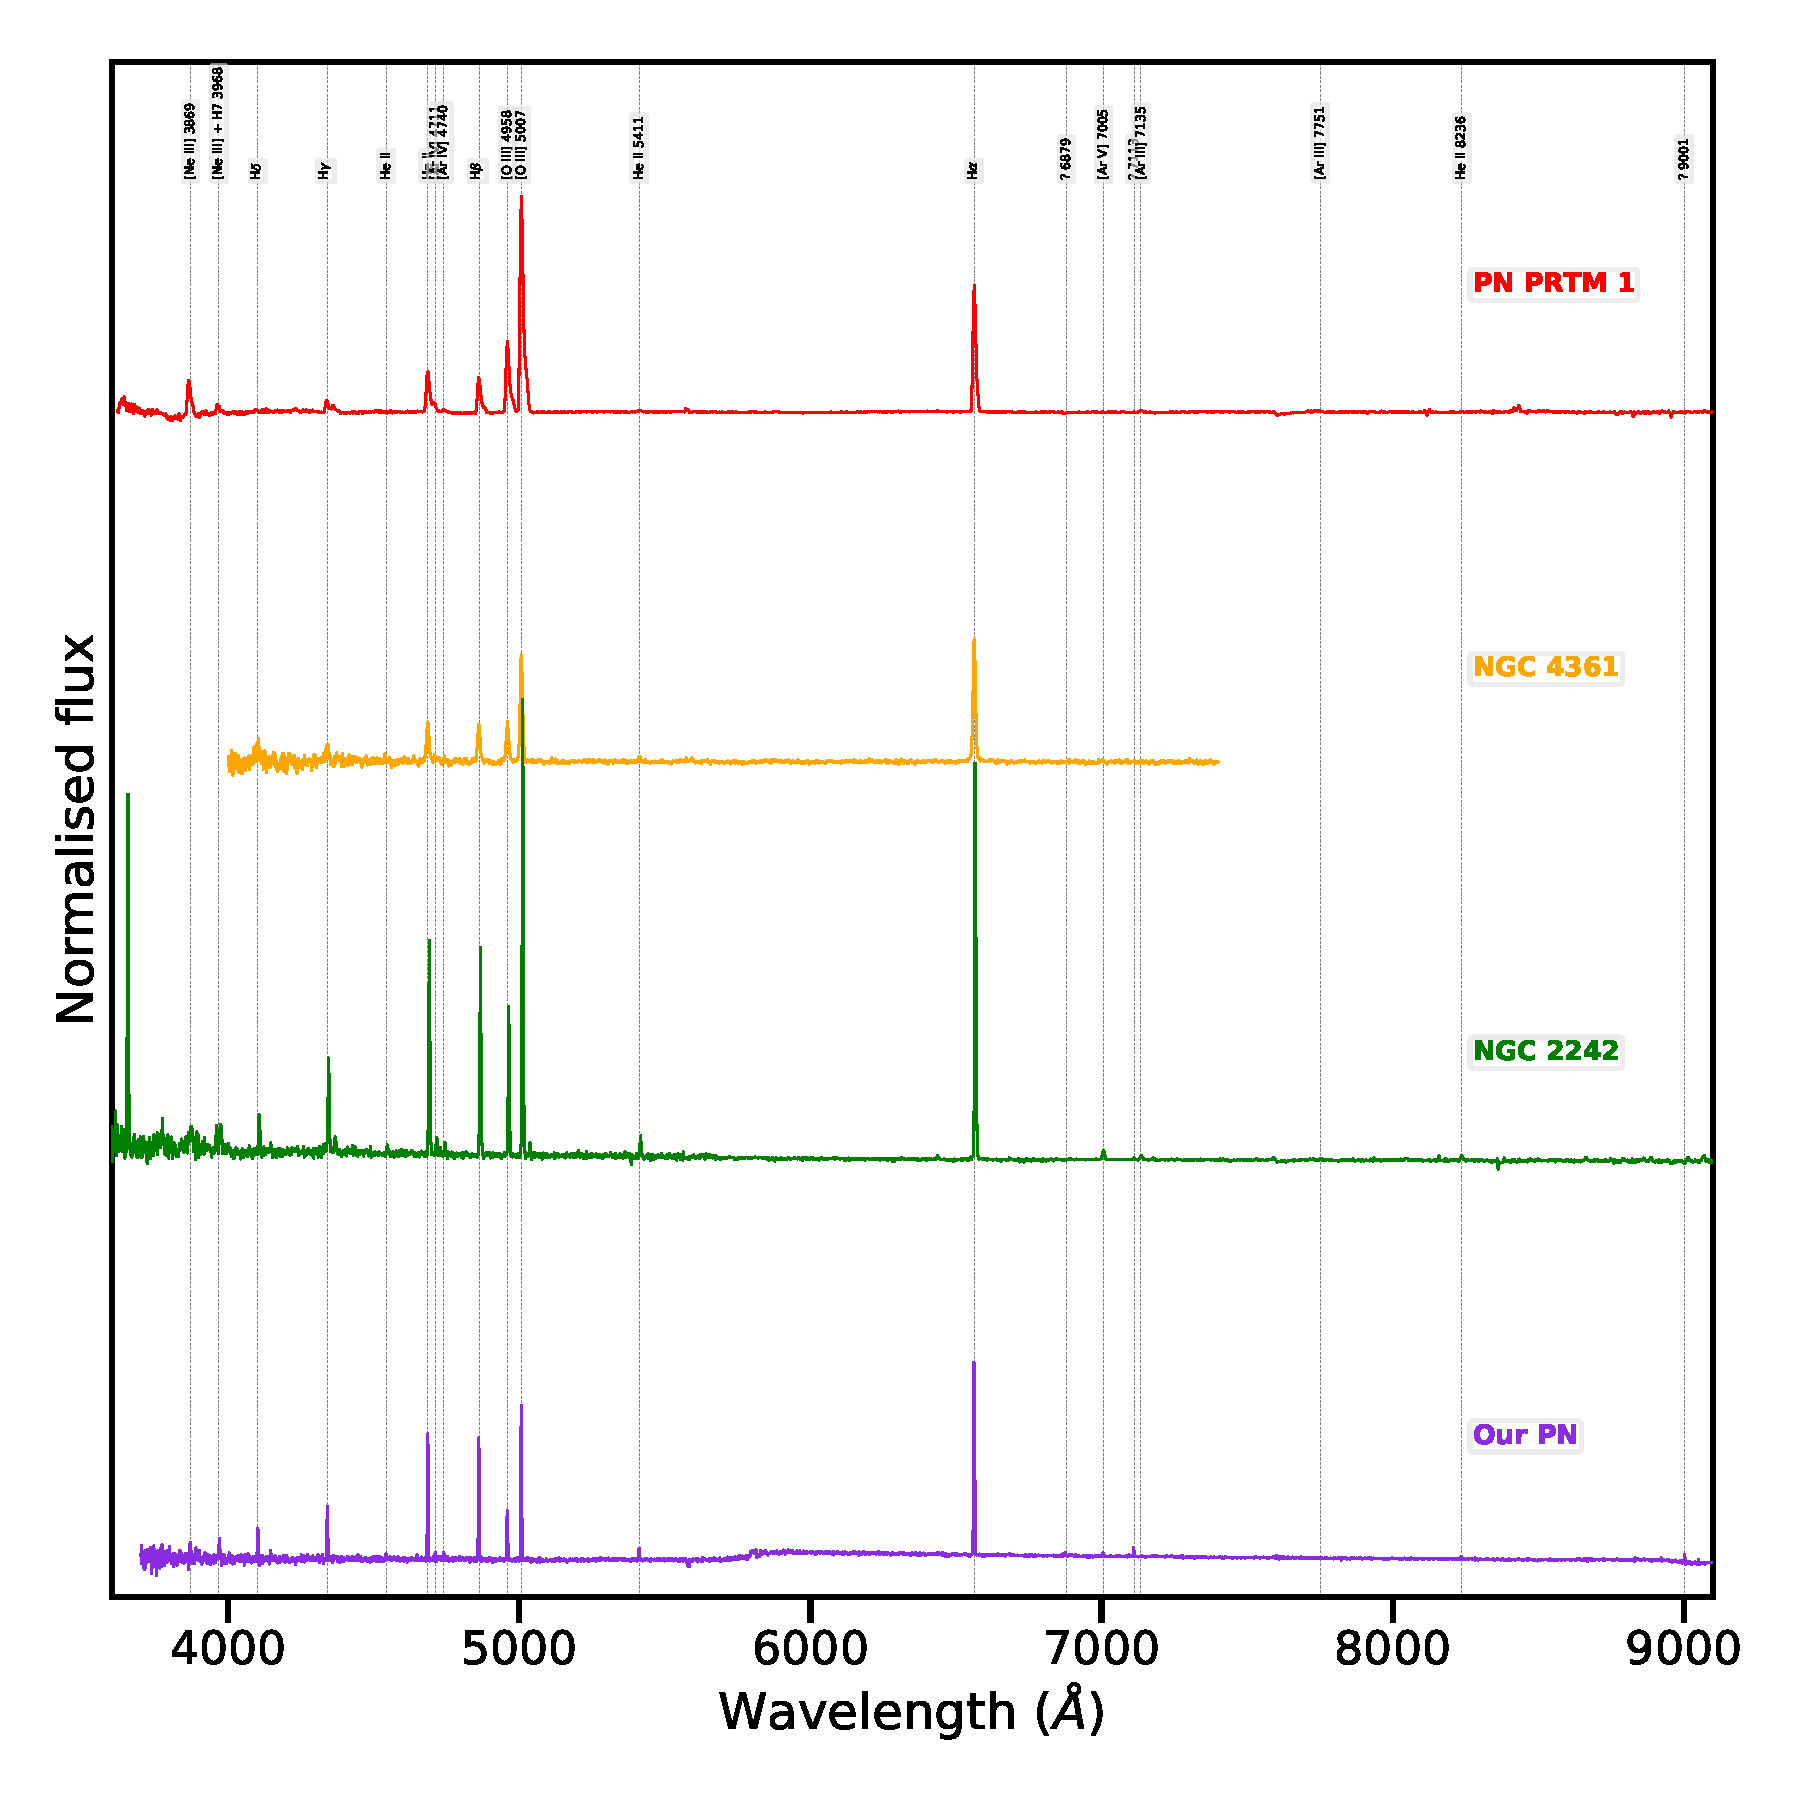
\includegraphics[width=\linewidth]{Figs/spectra-compare.pdf}
\caption{Spectra of 3 known PNe and the new PN. From upper to lower the ID of the
  sources are PN PRTM 1, NGC 4361, NGC 2242, and the recent discovery
  J020808.63+491401.0. The spectra have all been scaled and normalized
  for display purposes.} 
  \label{fig:compare-spectra}
\end{figure*}

%% In Fig~\ref{fig:compare-spectra} we are compare our PNe with
%% other high-ionization PNe (NGC 2242, NGC 4361 and PRTM 1).
%% Note that all three PNe are objects located at high latitudes,
%% this means that they belong to the halo Galactic.
%% All four spectra are very similar with the same Balmer lines,
%% the high-ionization lines and lacked the low-ionization lines.

\begin{figure}
  \centering
  \begin{tabular}{l l}
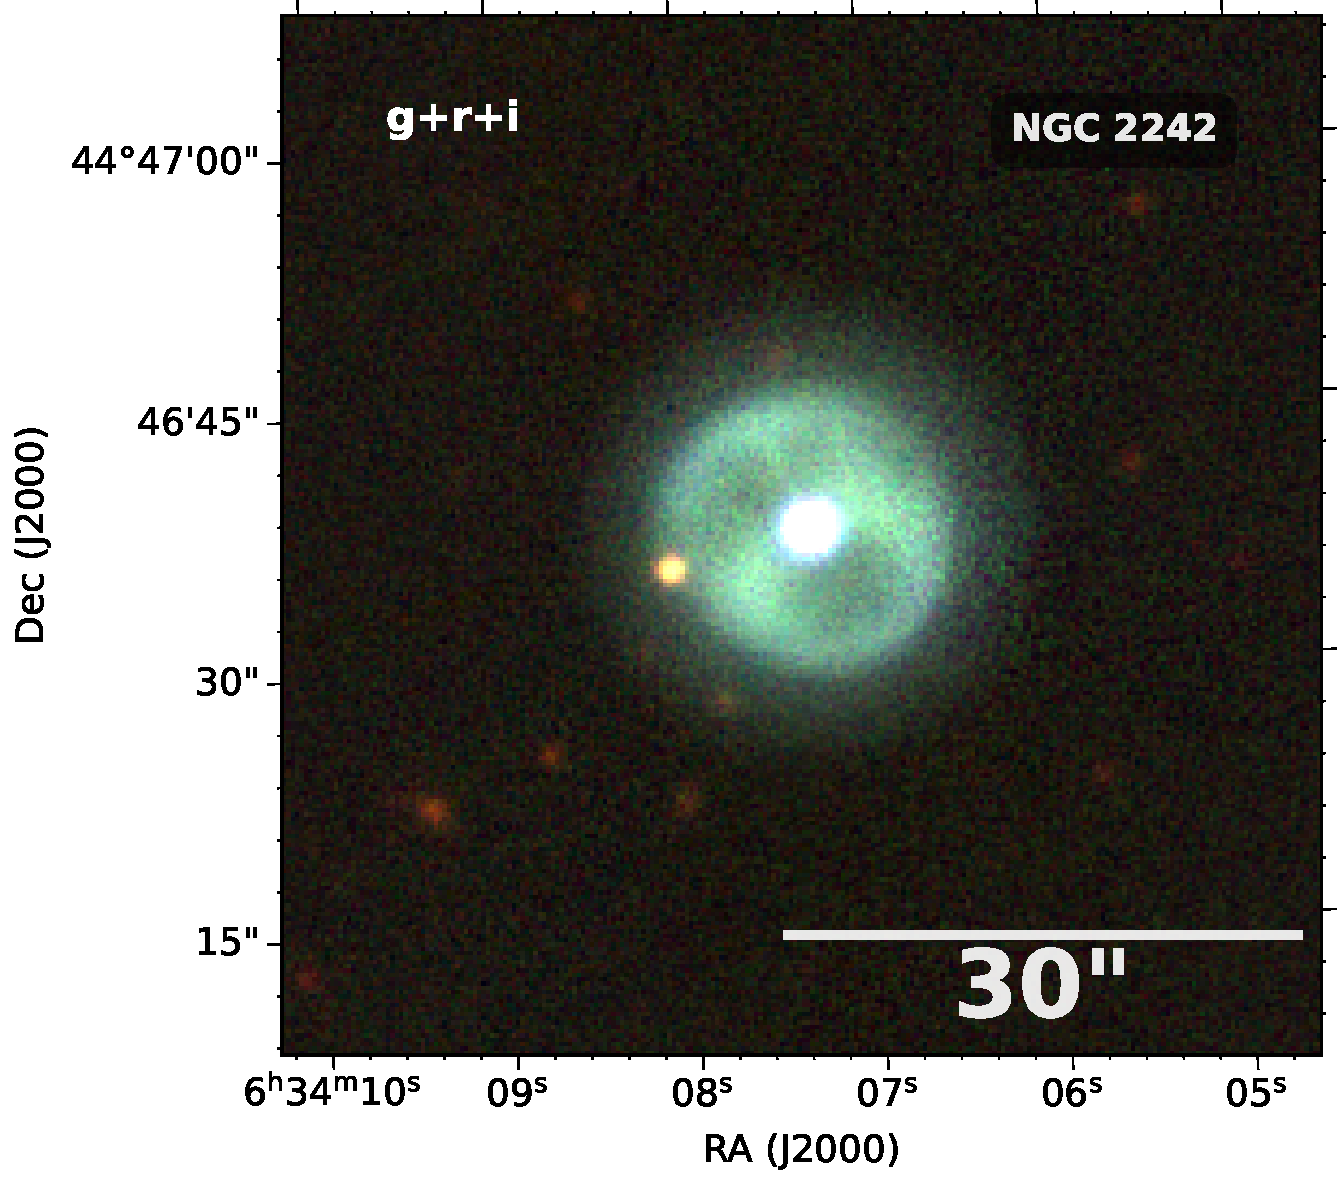
\includegraphics[width=0.52\linewidth]{Figs/cutout_rings.v3.skycell.2243.029.stk.i.unconv-irg-RGB.pdf}
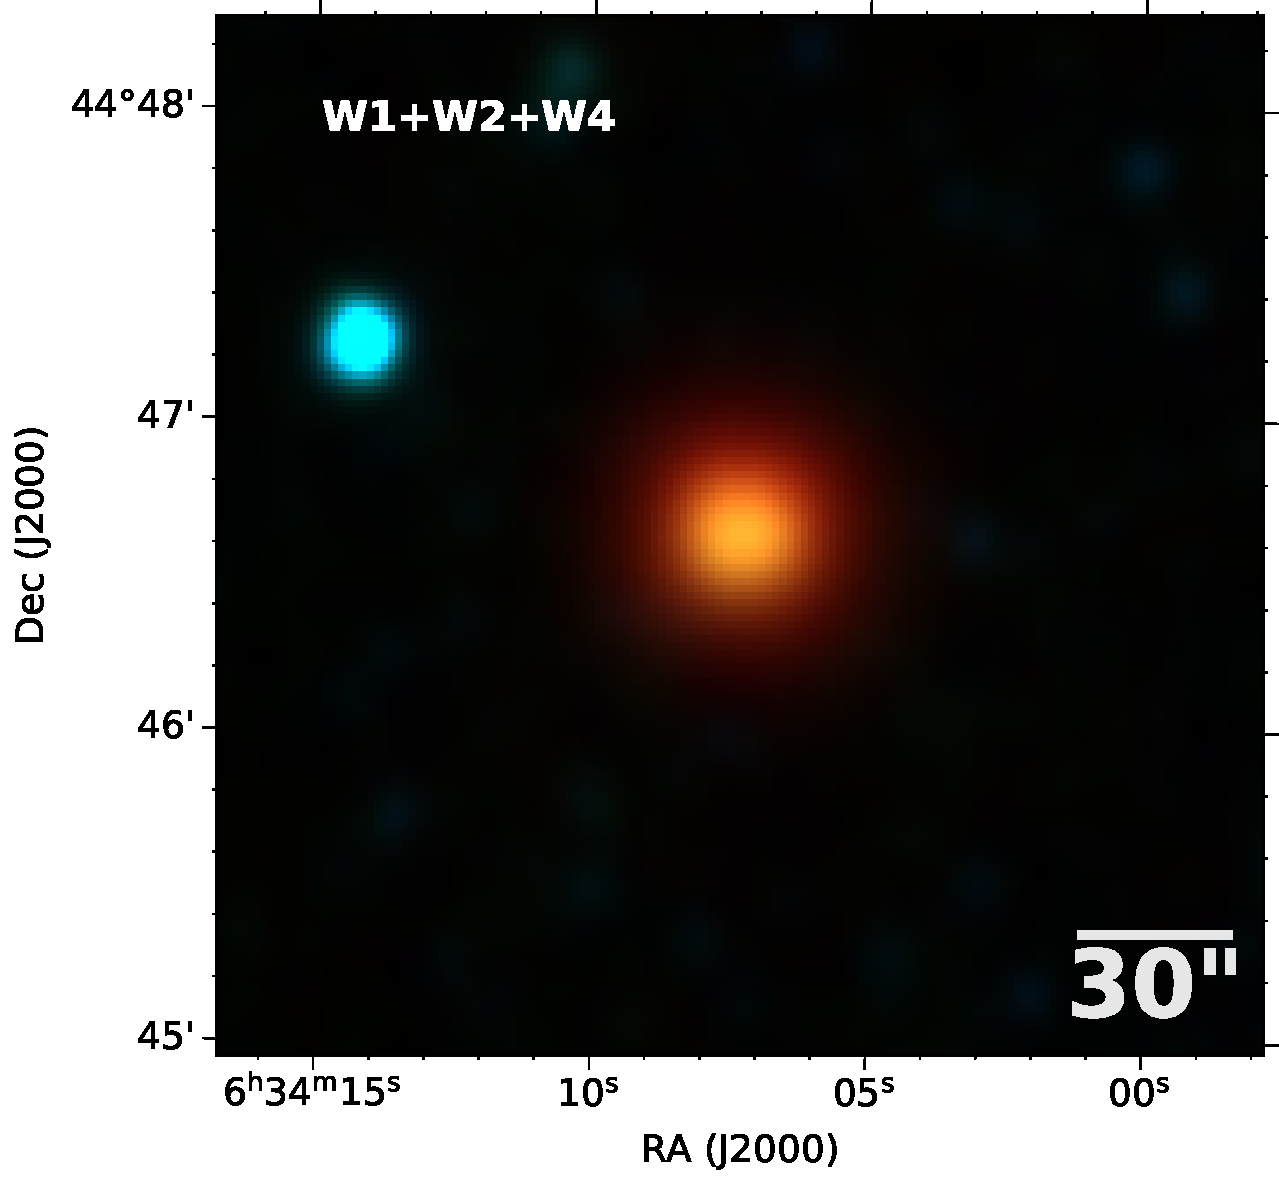
\includegraphics[width=0.5\linewidth]{Figs/0979p454_ac51-w4-int-3_ra98.53061791727998_dec44.77716333248_asec200.000-421-RGB.pdf}\\
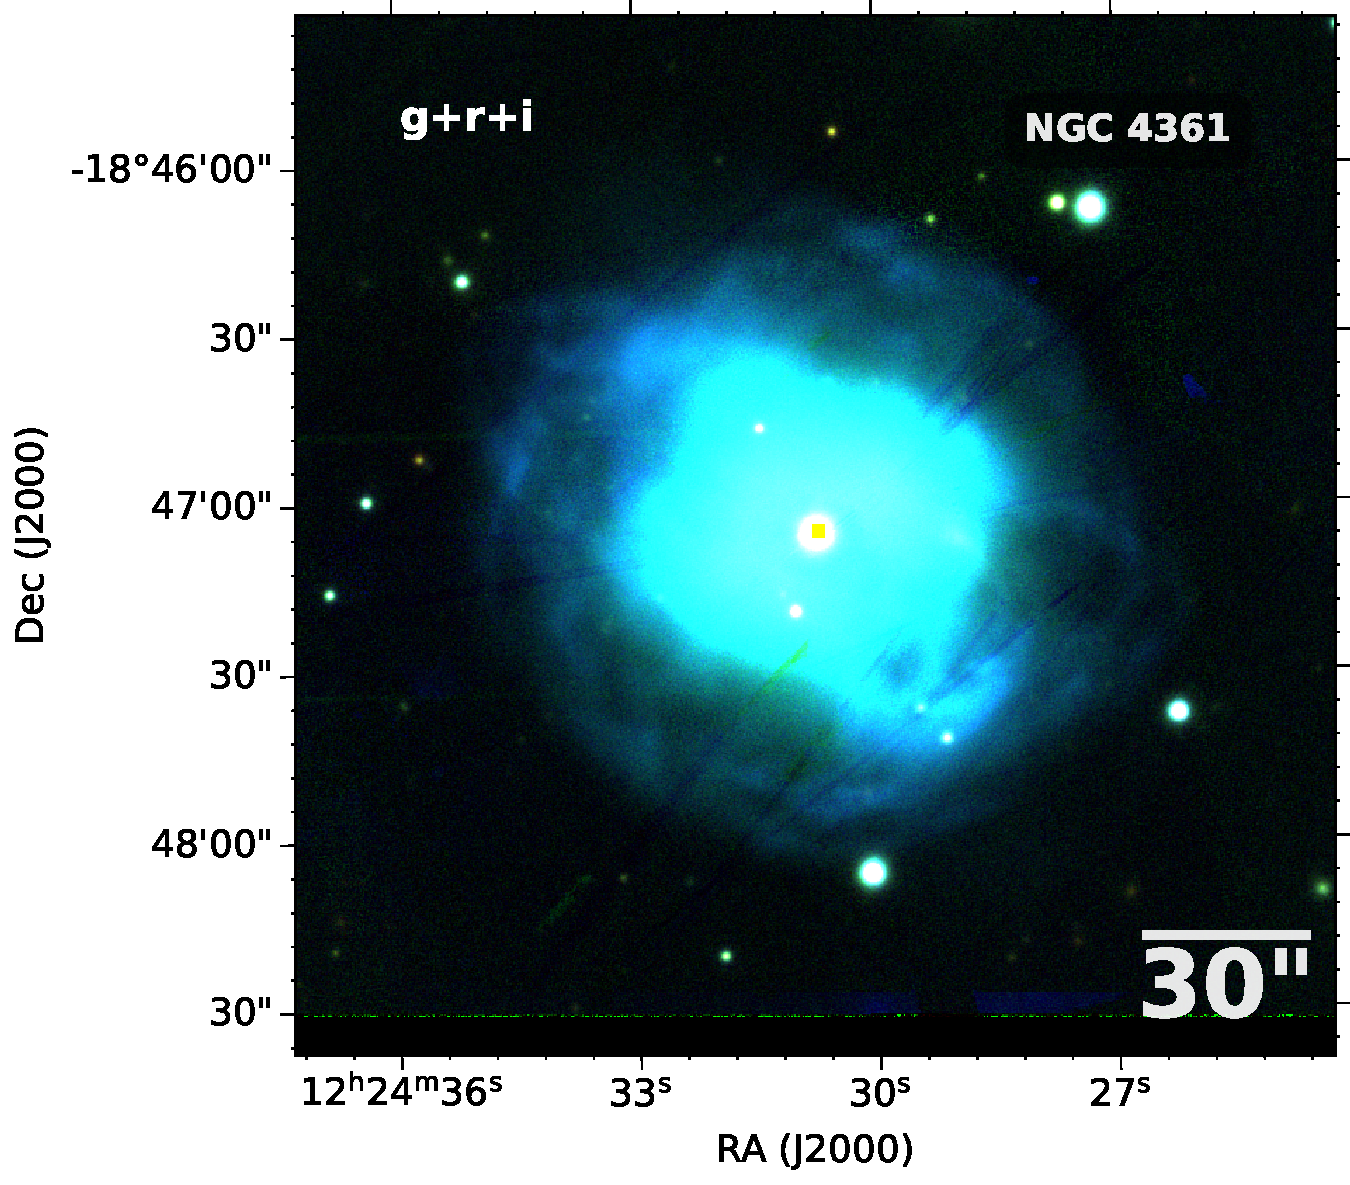
\includegraphics[width=0.52\linewidth]{Figs/cutout_rings.v3.skycell.0924.030.stk.i.unconv-irg-RGB.pdf}
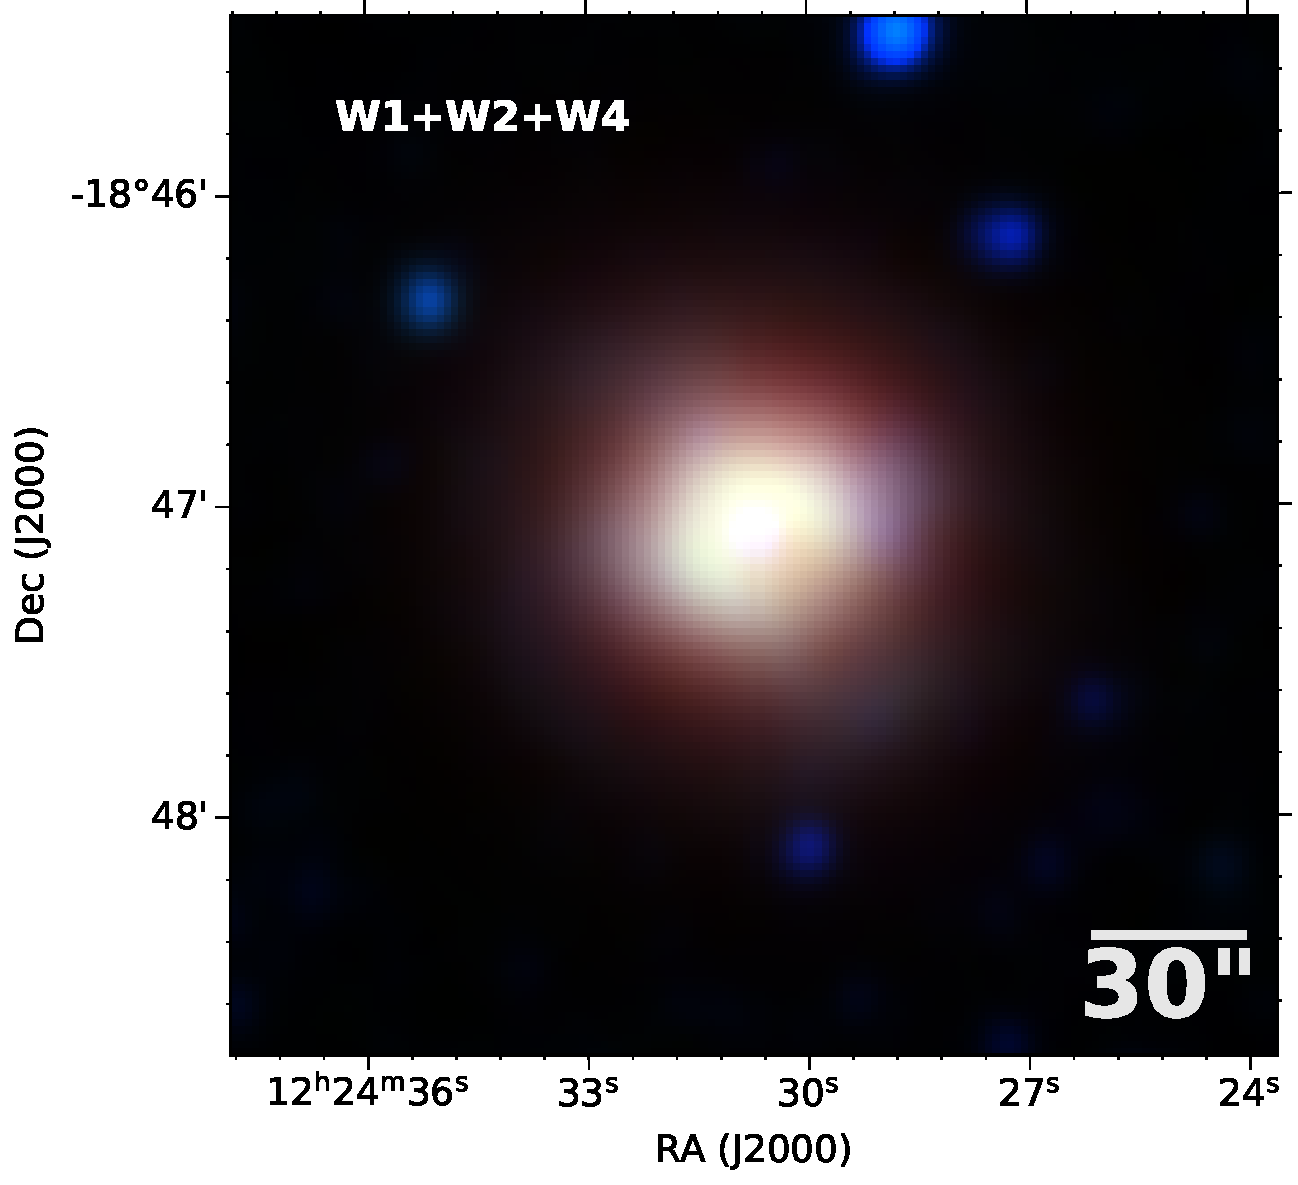
\includegraphics[width=0.5\linewidth]{Figs/1855m182_ac51-w4-int-3_ra186.12812938647002_dec-18.78487981564_asec200.000-421-RGB}\\
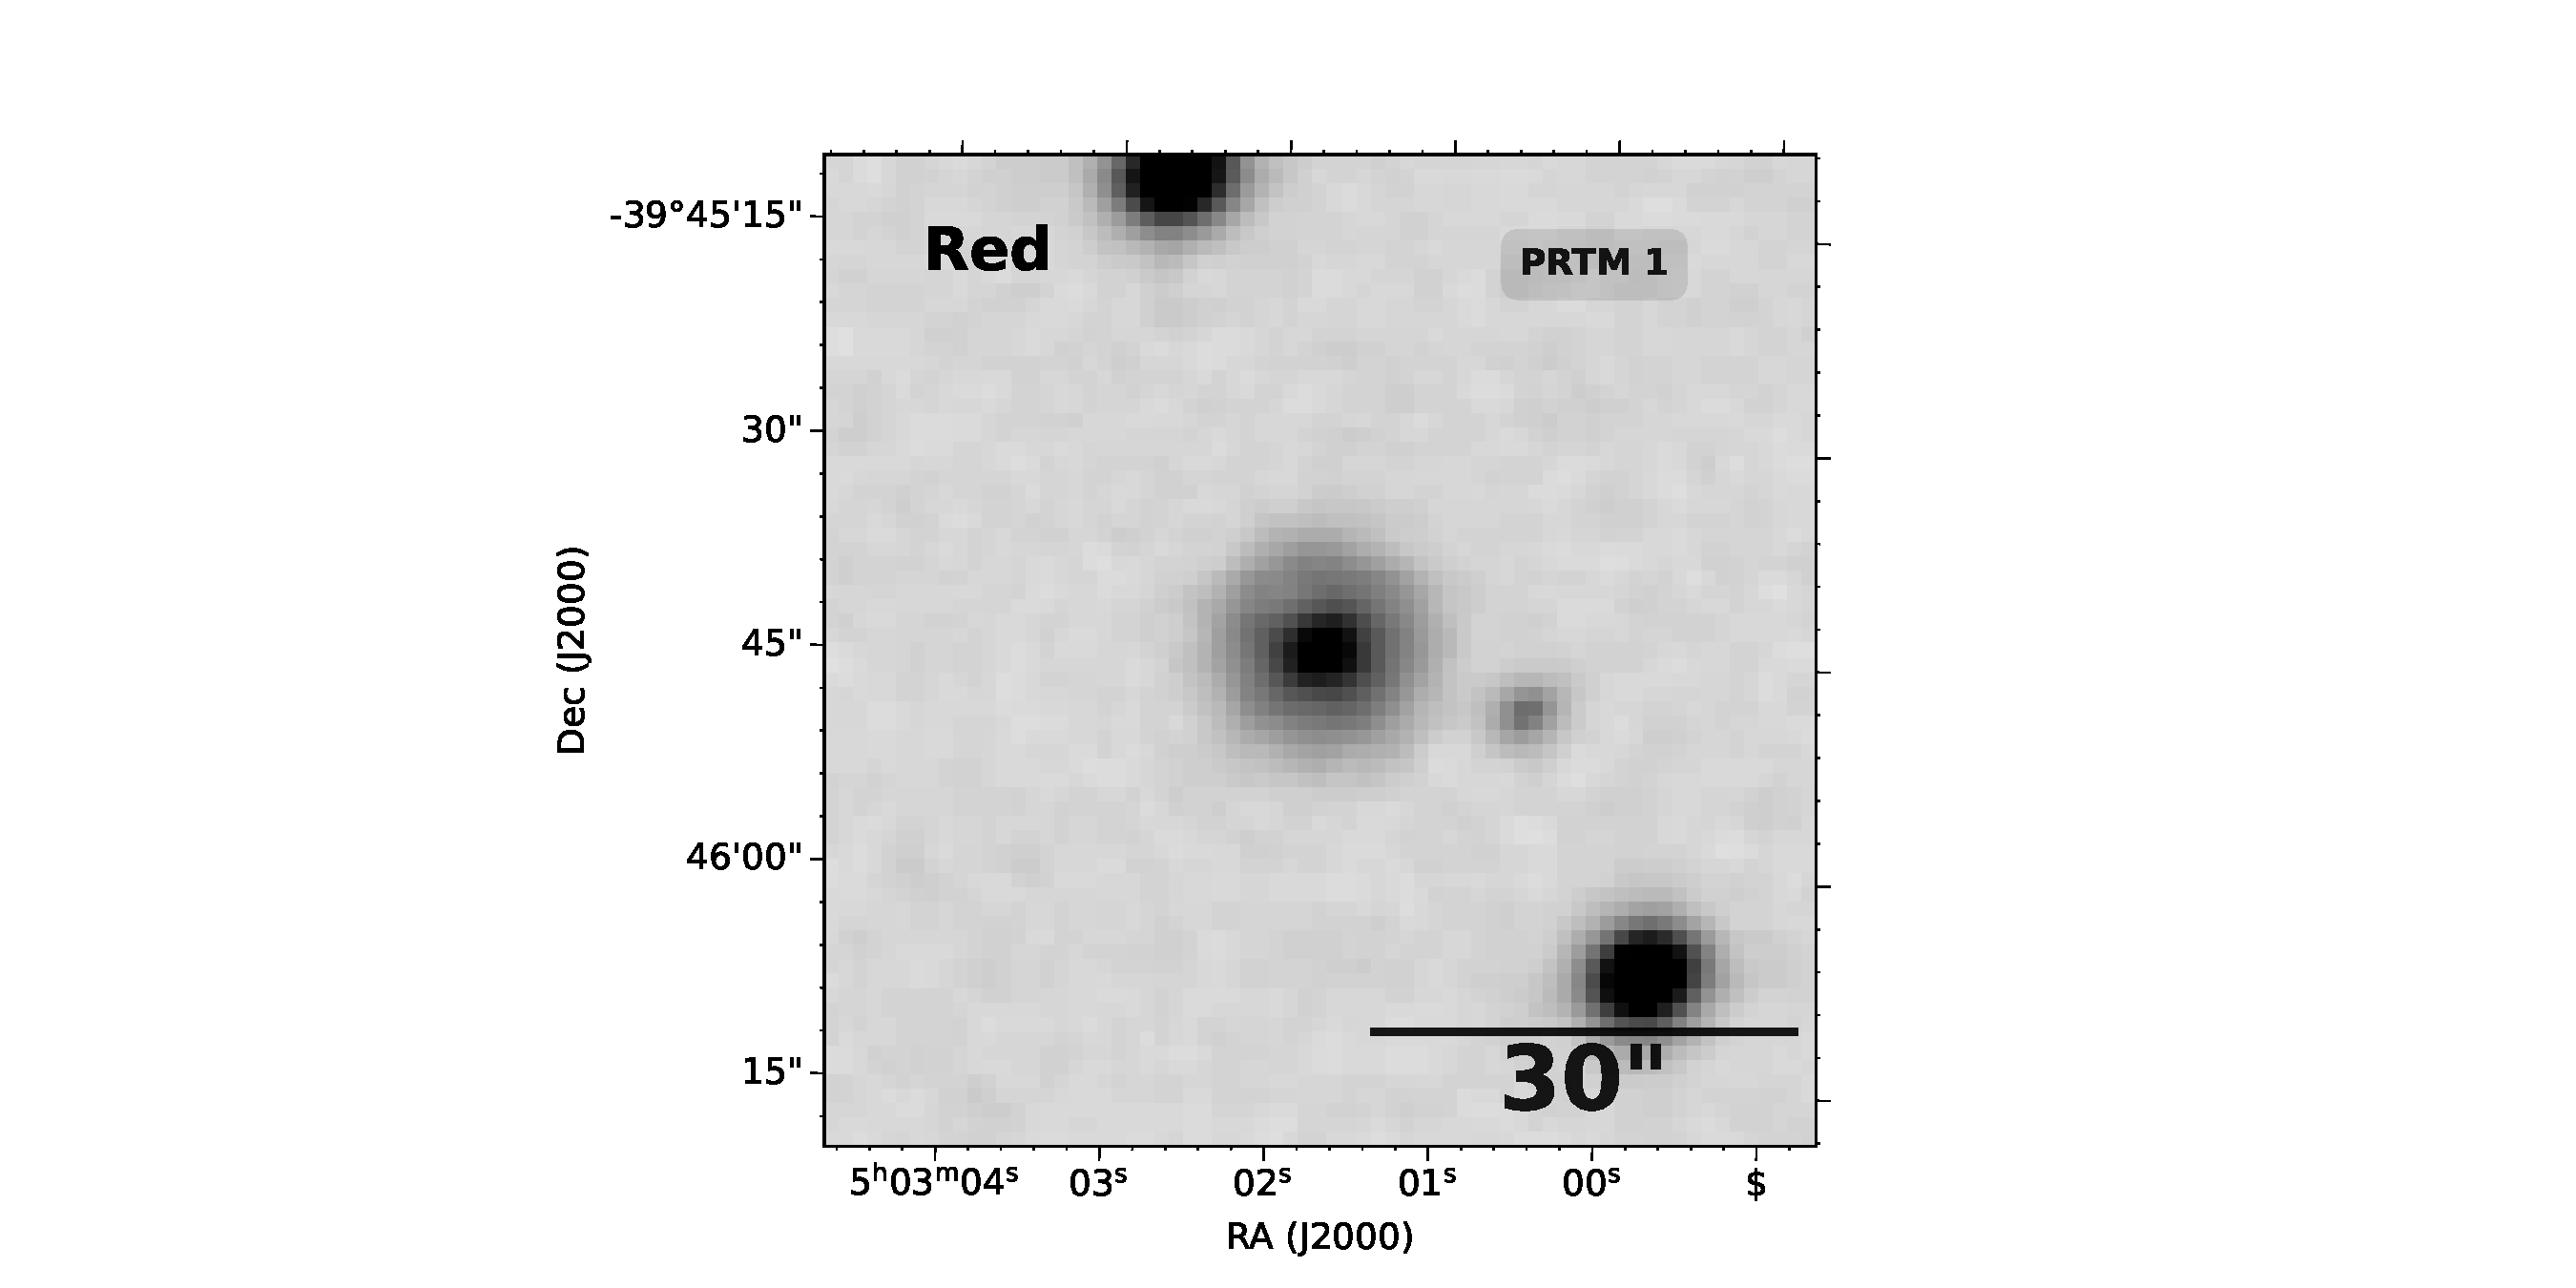
\includegraphics[width=0.535\linewidth, trim=280 10 330 10, clip]{Figs/dss_search_red.pdf}
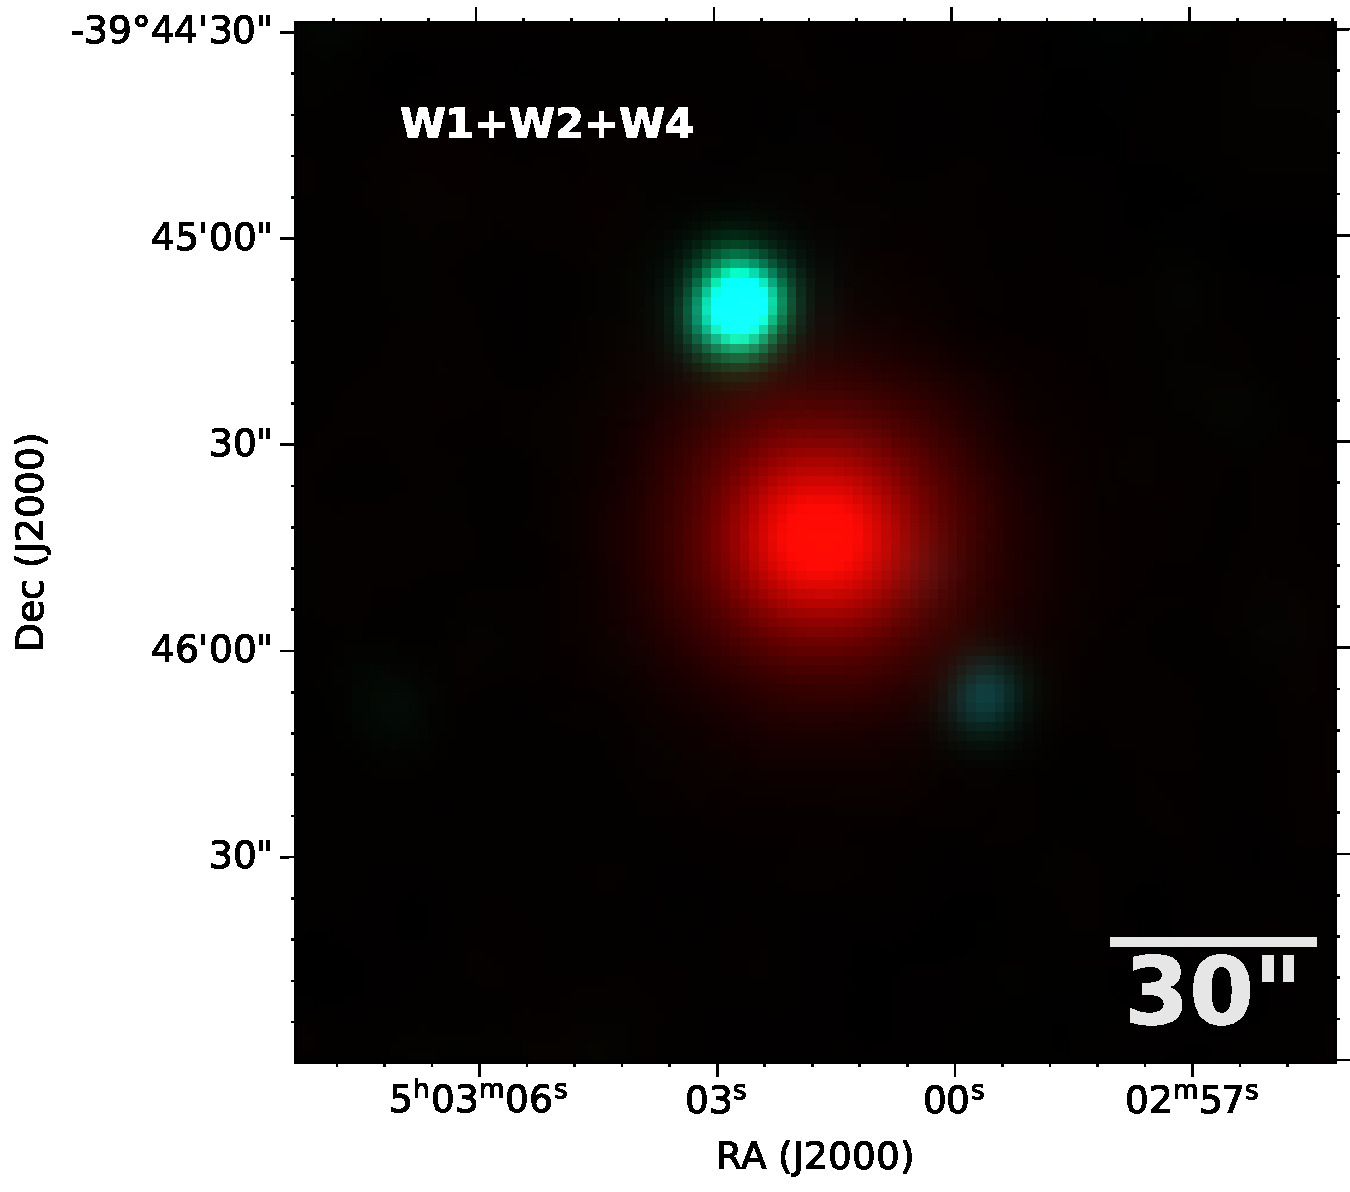
\includegraphics[width=0.47\linewidth, trim=58 0 0 0]{Figs/0754m394_ac51-w4-int-3_ra75.75721626934_dec-39.76236833917_asec150.000-421-RGB.pdf}\\

\end{tabular}  
  \caption{Optical (\textit{right}) and IR (\textit{left}) images of the 
    high-ionization PNe: NGC 2242 (\textit{upper}),  NGC 4361(\textit{medium}), and
    PN PRTM 1(\textit{bottom}).
    The optical coloured images were constructed by combining the
    $g$, $r$ and $i$ Pan-STARRS filters in the green, blue and red channels, respectively.
    The infrared RGB images were constructed by using the the W1 (3.368 $\mu$\,m), W2 (4.618 $\mu$\,m),
    and W4 (22.194 $\mu$\,m) WISE filters.} 
  \label{fig:images-known}
\end{figure}

Fig~\ref{fig:images-known} show the optical and IR images of the known planetary nebulae
presented in section ?? apparently all this PN have the same shape, e.g. are around like
the Lamost PN. Also in all them the central star is clearly perceptible like the LAMOST PN,
indicating, probably, the high temperature nature on their central star.

\subsection{Why is not a supernova?}
\label{sec:snr}

Two types of galactic emission line objects show high excitation
lines: planetary nebulae (\citealp{Bernard:2009}; \citealp{Guiles:2007})
and supernova remnants \citep{Sandstrom:2009, Ghavamian:2009}.
SNRs typically show very broad, high velocity ($v \geq 300$ km s$^{-1}$;
\citealp{Oliveira:2011}, \citealp{Fesen:2010}), emission lines,  produced by the
high velocity shock waves \citep{Fesen:1985, Fesen:1996, Stupar:2007}. 
PNe, on the other hand, are characterized by narrow emission lines
arising from the low-velocity expanding outer layers \citep{Balick:2002, Gorny:2009}.
We have estimate FWHM < 300 km s$^{-1}$ for the lines of J020808.63+491401.0, indicating
narrow emission lines.

The absence of high velocity optical emission lines and the lack
of detected [S II] emission, which would indicate the presence of shock-heated gas
typically of SNRs, suggests that the object is most likely a high-excitation PN.


\section{Modeling the observed LAMOST spectra}
\label{sec:model}

% Example table
\begin{table}
	\centering
	\caption{Best-fit {\sc cloudy} model parameters for LAMOST J020808.63+491401.0.}
	\label{tab:example_table}
	\begin{tabular}{lc} % four columns, alignment for each
                \hline
		\hline
		Parameter & Value \\
                \hline
		$\log(T_{\mathrm{BB}}) (\mathrm{K})$  & 05.15  \\
		$\log(\mathrm{luminosity) (erg~s^{-1})}$ & 36.79 \\
		$\log(\mathrm{Hden) (cm^{-3})} $ & 03.40  \\
                 $\log(\mathrm{R_{in}) (cm)}$ &  16.60\\
                $\log(\mathrm{R_{out}) (cm)}$ & 17.05 \\
                Distance (kpc) & 02.31  \\
                $\log(\mathrm{He/H})$ & -0.92 \\
                $\log(\mathrm{C/H})$ & -4.15 \\
                $\log(\mathrm{N/H})$ & -4.72 \\
                $\log(\mathrm{O/H})$ &  -3.83\\ 
                $\log(\mathrm{Ne/H})$ & -4.58 \\
                $\log(\mathrm{Si/H})$ & -5.00\\ 
                $\log(\mathrm{S/H})$ &  -6.00\\ 
                $\log(\mathrm{Ar/H})$ & -6.24\\
                 \hline
                 $\chi^2_{\text{min}}$ & 18.10  \\
                 
                 \hline
	\end{tabular}
\end{table}

Given the small number of observational constraints, we adopt a very
simple model of a planetary nebula which consists of a homogeneous
gaseous sphere surrounding an hot star radiating as a black body,
Here we attempt to model low-resolution spectra of J020808.63+491401.0.
Despite the LAMOST spectra are not in physical flux unity,
they are in calibrate flux relative. This means, it is possible compare it with other
spectra in physical units. For that, we thought, it is pertinent to
compare the LAMOST spectra of our PN with models.

The observed spectrum was modelled by using the {\sc cloudy}
photo-ionization code version c22.01 \citep{Ferland:2017}. {\sc cloudy}
has been applied to derive the physical characteristics and elemental
abundances of the PN, on which were considered by comparing with known
high-ionization PNe. This code is based on detailed microphysics to
simulate the physical conditions of non equilibrium gas clouds exposed to
an external radiation field. It solves the thermal, statistical, and chemical
equilibrium equations self-consistently, from non-local thermodynamic
equilibrium (NLTE), illuminated gas clouds. Currently, it uses 625
species including atoms, ions, and molecules and five distinct
databases: H-like and He-like isoelectronic sequences \citep{Porter:2012},
Stout \citep{Lykins:2015}, CHIANTI \citep{Landi:2012},
LAMDA \citep{Schoier:2005}, and the H2 molecule
\citep{Shaw:2005} to model the spectral lines. All the known
important ionization processes, e.g., photo, Auger, collisional
and charge transfer and recombination process, namely,
radiactive, di-electronic, three-body recombination, and charge
transfer are included self-consistently. {\sc cloudy} predicts both
the intensities and column densities of a very large number
($\sim 10^{4}$) of spectral lines covering the whole electromagnetic
range, from non-local thermodynamic equilibrium (NLTE),
illuminated gas clouds by solving the equations of thermal and
statistical equilibrium for a given set of input parameters. More
details about {\sc cloudy} could be found in \citet{Ferland:2013}
and \citet{Pandey:2022}. The code uses a set of input parameters to compute the
ionization, thermal, and chemical state of a non-equilibrium gas cloud
illuminated by a central source and predict the resulting spectra. 
In the past, \citet{Vejar:2019} used {\sc cloudy} to produce
synthetic spectra of PNe to simulate the Broadband photometry
of Large Synoptic Survey Telescope(LSST). In the same way, a grid of modelled
halo galactic PNe were performed to simulate the J-PLUS and S-PLUS photometry
to developed new color criteria to find for PNe based on these surveys
by \citet{Gutierrez-Soto:2020}.
In this order of ideas, we used {\sc pyCloudy} \citep{Morisset:2013} a
package python\footnote{\url{https://sites.google.com/site/pycloudy/home}} which
is a set of tools to deal with photoionization code {\sc cloudy} (\url{www.nublado.org}),
which was used to create a set of inputs for the model and deal with the output files.

We consider a central ionizing source surrounded by a spherically symmetric
gaseous material on which dimensions are determined by the inner ($R_{\mathrm{in}}$) and
outer ($R_{\mathrm{out}}$) radii (cm). The central ionizing radiation is assumed to have a
black-body shape with temperature T$_{\mathrm{BB}}$ (K) and luminosity L
(ergs$^-1$). We assume spherical geometry for the nebula, a uniform filling factor of unity.
Using {\sc pyCloudy} we iterative generated the input files for the models.
Many models were generated with the intention of finding the best fit.
In agreement with the LAMOST spectra and similarity with theses high-ionization PNe
(see \ref{fig:compare-spectra}).
We considered a set of effective temperature between 10$\times10^4$ and 20$\times10^4$
in step of 10$\times10^3$, luminosities from 400$L_{\odot}$ to 10100$L_{\odot}$ in steps
of 300$L_{\odot}$ and hydrogen density from 500 to  6000cm$^{-3}$ in step of 500.
We note that the spectra of LAMOST J020808.63+491401.0 is particularly quiet similar to the
spectrum of NGC2242, so we first adopted the abundances (mainly of NGC 2242) of it and after
we change the value of He and Ar to get a better match with the observed spectra.
We also adopted inner and outer radius of that showed very good. We used the input
distance those geometrical distances of the object estimated by \citet{Bailer:2021} based on
the parallax of GAIA of 2.31 kpc.
After to produce the models and given that the observed spectra could be affected by
dust interstellar extinction, we reddened each modelled 1D-spectra applying the
reddening curve of R(V) = 3.1, and using colour excesses, E(B-V), from 0.0 to 0.1 in
step of 0.01, and also for 0.2. This was made by implementing the python
package \texttt{dust\_extinction}\footnote{\url{https://dust-extinction.readthedocs.io/en/stable/#}}.
This produced more than 40$\times10^3$ models. Fig~\ref{fig:spectra-obs-model} shows a
comparison between LAMOST spectra and a {\sc cloudy}. %% This model was taken from a grid of
%% models that reproduce spectra form the Galactic halo. For this, it don't exist a real matches
%% between the two spectra. I will a perform a grid of PN models that better reproduce the
%% LAMOST spectra of our candidate. However, almost all the line are reproduce with this model,
%% that could be interesting, because the temperature effective of this model is
%% 130$\times10^3$K, indicating a very high excitation object.
%% Maybe, it will be good idea estimate ratio lines to confirm that! is it possible with this
%% spectrum? The observed spectrum and the modeled spectrum were matched using fluxes relative
%% to the H{$\beta$} emission line.

\subsection{The best fit models}
\label{sec:best-fit}

\citet{Helton:2010, Mondal:2018, Pavana:2019, Mondal:2020, Pandey:2022a, Pandey:2022b}
implemented the $\chi^2$ to compare observed spectroscopic data,
mainly novas sources, with modelled {\sc cloudy} spectra to find the best
fit models. Following these authors, we choose the final best models
after many iterations of multiple test models based on varying the input parameter,
as was showed before, by using the criteria of minimum chi-square.
To do that, we compare the model generated lines with the fluxes of the observed lines.
This allows determined automatically the goodness of the fit by
calculating $\chi^{2}$ of the models given by the following relation,

\begin{equation}
  \chi^{2} = \sum^{n}_{i = 1} \frac{(M_i - O_i)^2}{\sigma^{2}_i}
  \label{eq:chi}
\end{equation}

where $M_i$, $O_i$ and $\sigma^{2}_i$ are the modelled line flux ratios, the observed line flux
ratios and uncertainty in the observed line flux ratios, respectively. We define the minimum
$\chi^{2}$ of the new PN as

\begin{equation}
   \chi^{2}_{\text{min}} = \sum^{9}_{i = 1} \frac{(M^{\text{best}}_i - O_i)^2}{\sigma^{2}_i}
  \label{eq:chi-red}
\end{equation}

the number 9 in sum symbol indicates the number of parameters used to estimate the  $\chi^{2}$
value. In this case, we used the 9 flux lines most intense.
This lines are [Ne III] 3967.5 \AA, H$\delta$, H$\gamma$, He II 4685.9 \AA, H$\beta$, [O III] 4958.9 \AA,
[O III] 5006.8, He II 5411.7 \AA~and H{$\alpha$}.
%% where $\nu$ is represents the number of degrees of freedom (DOF), which is estimate
%% by implementing $\nu = n - n_p$, with $n$ and $n_p$ being the number of observed lines
%% used to estimate $\chi^{2}$ and the number of parameters, respectively. Note that for a reasonably
%% fit, the value of $\chi^{2} \sim \nu$. This means that the value of $\chi^{2}_r$ should be low,
%% usually between 1 and 2. 

The flux lines of each line were measured interactively by fitting a 1D-Gaussian using
the 10 $\AA$ centered on the line and integrate over this best fit Gaussian within more
or less 3$\sigma$ interval. Being $\sigma$ the standard deviation of the individual
line fit Gaussian. We found automatically the parameters to fit the best 1D-Gaussian model
using the function \texttt{estimate\_line\_parameters} from \texttt{Astropy specutils.fitting}
package\footnote{\url{https://specutils.readthedocs.io/en/stable/index.html}}.

The uncertainty in the flux ratios of the observed lines were computed following the
equation presented by \citet{Tresse:1999}:

\begin{equation}
  \sigma_{F} = \sigma_{c} D \sqrt{2N_{\text{pix}} + \frac{\text{EW}}{D}
  \label{eq:err-sigma}
\end{equation}

respectively, where $\sigma_{c}$ is the mean standard deviation per pixel of
the continuum on each side of the line, $N_{\text{pix}}$ is the number of pixels
under the line and $D = 1.0009 \AA$ pixel$^{-1}$ is the spectral dispersion.

\begin{figure*}
\centering
  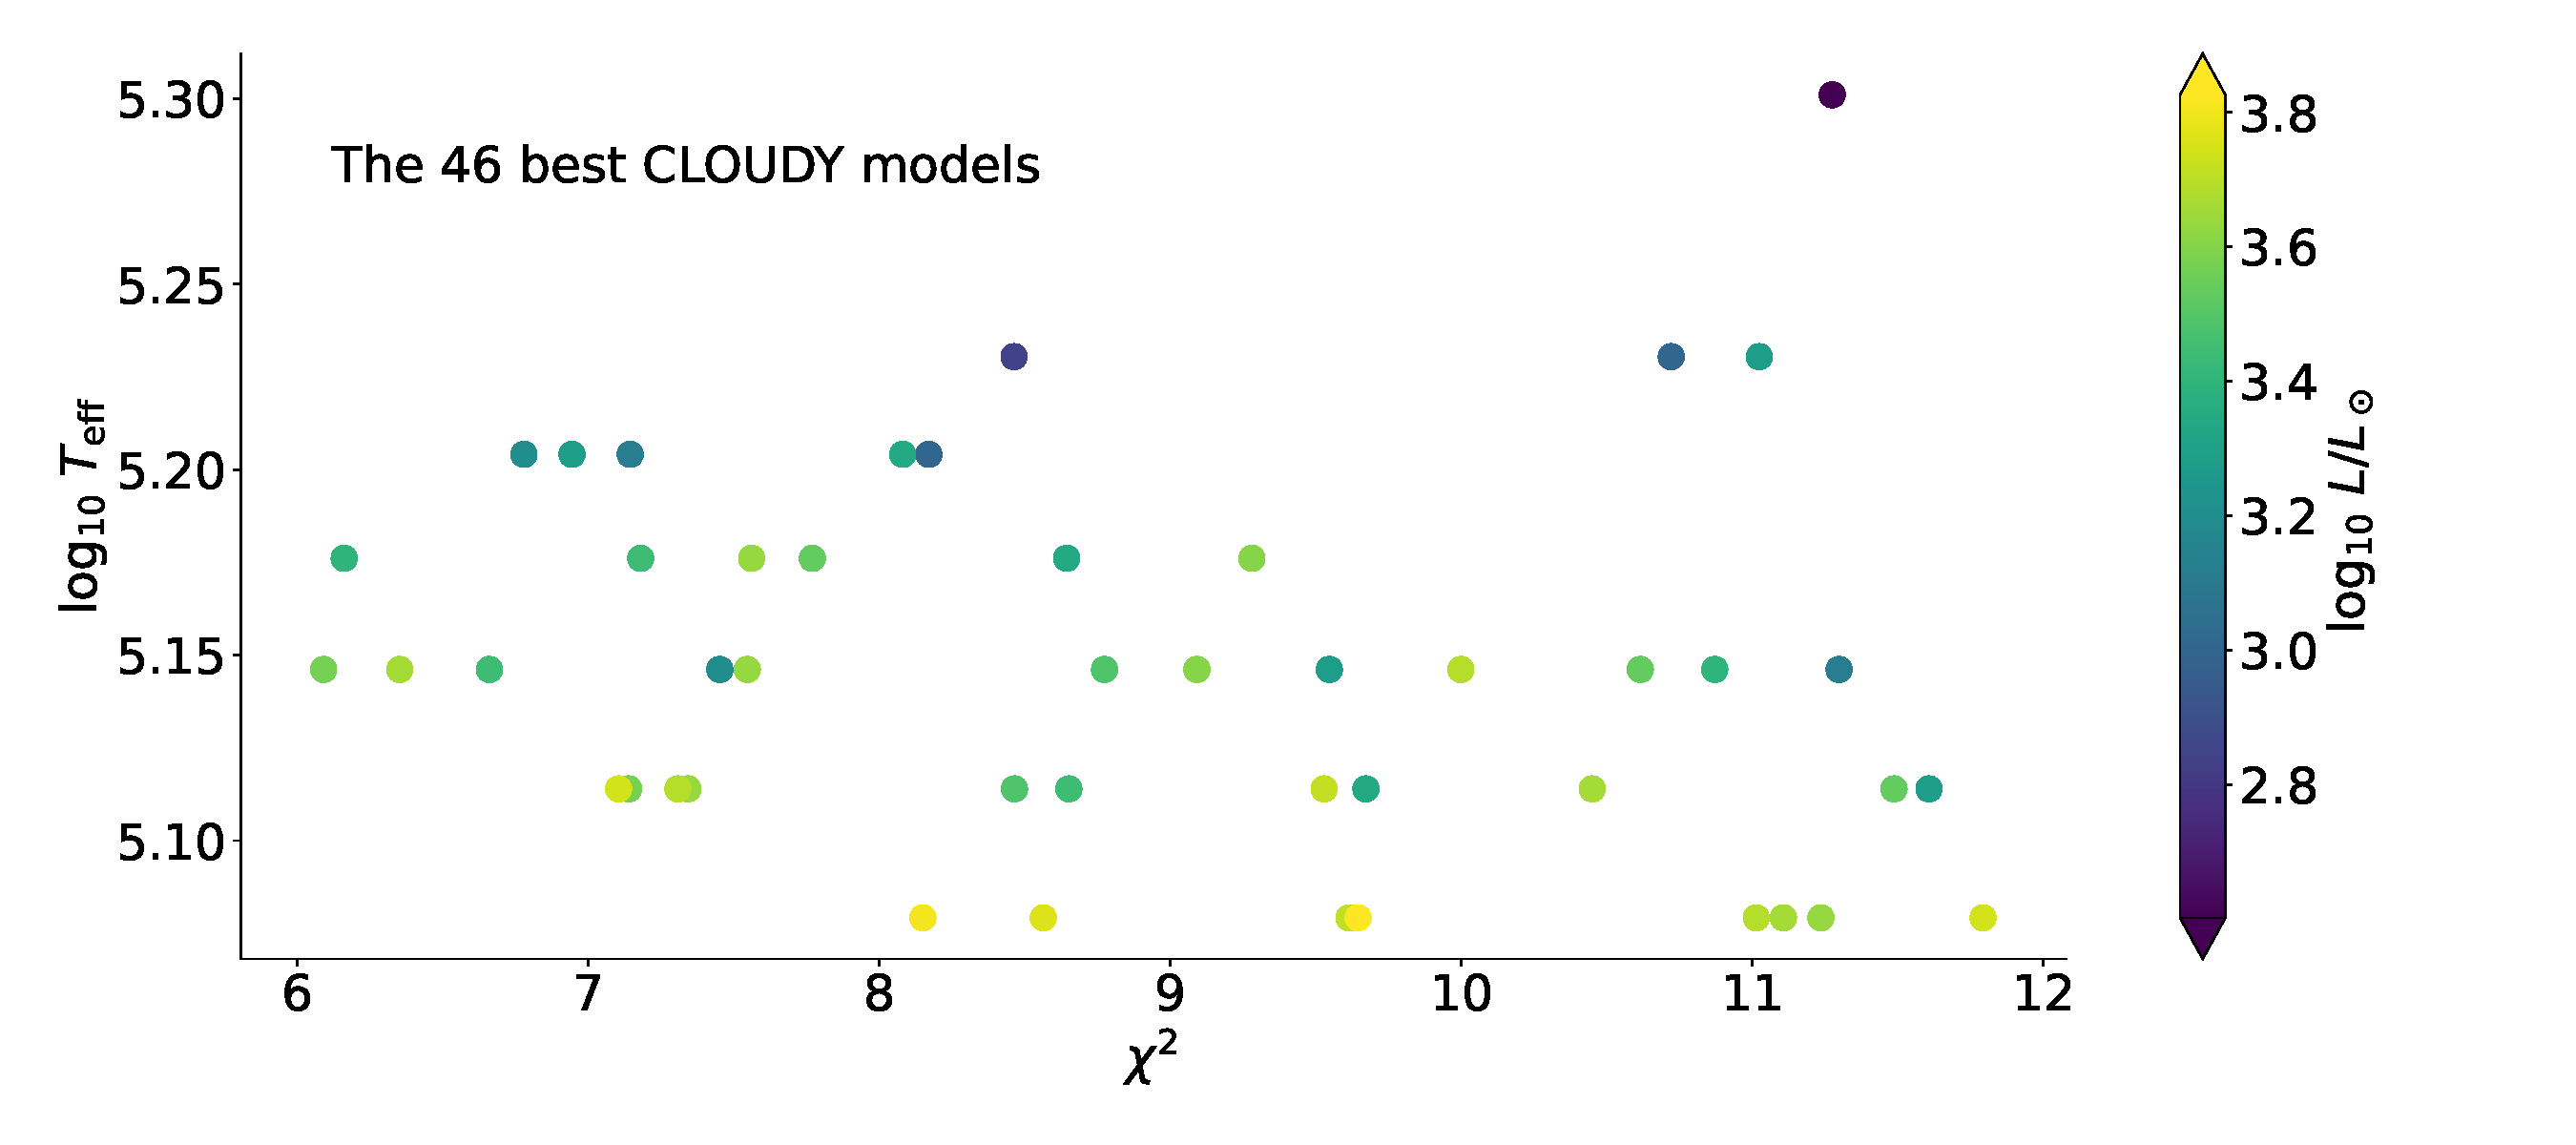
\includegraphics[width=\linewidth]{Figs/chi-temperature.pdf}
  \caption{The effective temperature (in logarithm scale) versus $\chi^2$ plot.
    The 46 best fitted model on which the $\chi^2_r$ have between 1 and 2.} 
  \label{fig:chi}
\end{figure*}

% Example table
\begin{table*}
	\centering
	\caption{Observed and best-fit {\sc cloudy}  model line fluxes for
          LAMOST J020808.63+491401.0.}
	\label{tab:abundances}
	\begin{tabular}{lcccc} % four columns, alignment for each
                \hline
		\hline
		Line & $\lambda$(\AA) & Observed Flux  & Model  Flux & $\chi^{2}$  \\
		\hline
		[Ne III] + H7 3968  & 3967.46 & 0.26 $\pm$ 0.068 & 0.29 & 0.27\\
		H{$\delta$} & 4101.74 & 0.29 $\pm$ 0.053 & 0.35 & 1.02\\
		H{$\gamma$}  & 4340.71 & 0.48 $\pm$ 0.047 & 0.58 & 5.37 \\
                He II & 4685.99 & 1.04 $\pm$ 0.061 & 1.05 & 0.01\\
                H{$\beta$} & 4861.33& 1.00 $\pm$ 0.055 & 1.00 & 0.00\\
                $[\text{O III}]$ &4958.91 & 0.44 $\pm$ 0.031 & 0.48 & 1.63  \\
                $[\text{O III}]$ & 5006.84& 1.21 $\pm$ 0.060 & 1.20 & 0.09 \\
                $[\text{Fe III}]$ & 5412.12& 0.13 $\pm$ 0.016 & 0.17 & 4.32\\
                H{$\alpha$} & 6562.85& 2.33 $\pm$ 0.097 & 2.56& 5.39
                \hline
	\end{tabular}
\end{table*}

The $\chi^{2}_{min}$ values indicates that the {\sc cloudy} generated
spectra model match well with the observed spectra. Even while our model reproduces
a wide variety of observable effects, the phenomenology has certain limits.
In this sense, from about 40000 models generated, we choose those that
match very wells with the spectra of J020808.63+491401.0,
the values of $\chi^{2}$ of the three best-fit spectra
are shown in the table~\ref{tab:abundances}. The three
models have values of $\chi^{2}$ between 1 and 2, satisfying
the criteria for an acceptable fit. Being the best model-fit ($\chi^{2}_{r} = 1.2$)
those which is the  planetary nebula spectrum model with the
most high effective temperature (T$_{\text{eff}}$ = 160$\times$10$^{4}$).

\begin{figure*}
\centering
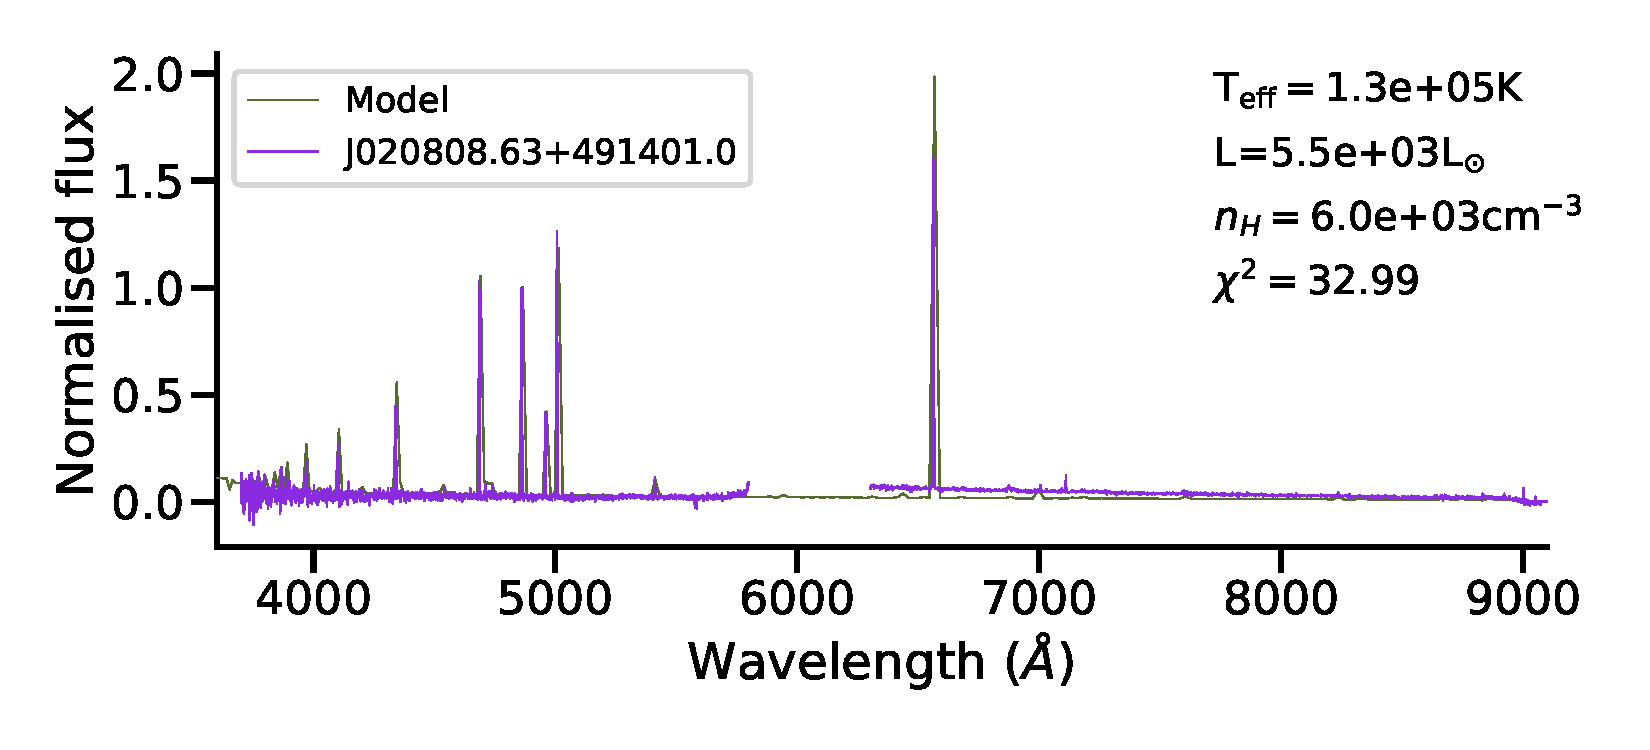
\includegraphics[width=\linewidth, trim=10 90 10 10, clip]{Figs/model_130000_37.32_3.78.pdf}
\caption{The three best fitted models, on which the $\chi^2_r$ value are 1.13, 1.59, 1.61.
  The spectra were normalised to H{$\beta$}.} 
  \label{fig:spectra-obs-model}
\end{figure*}

\section{Comparison with post-AGB stellar evolution tracks}
\label{sec:tracks}

\begin{figure}
\centering
  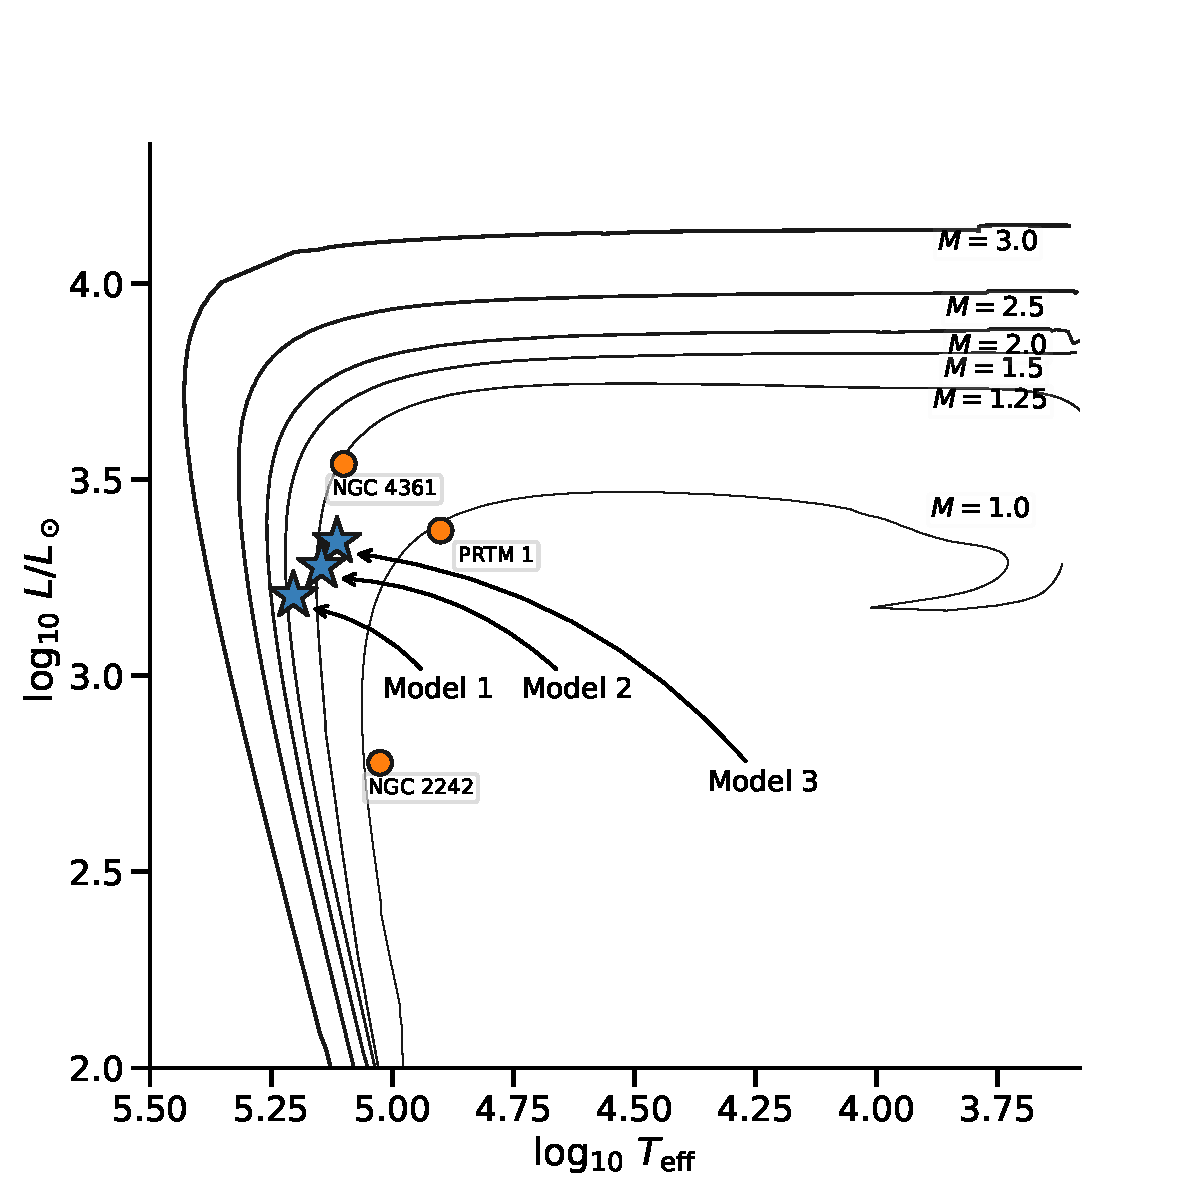
\includegraphics[width=\linewidth]{Figs/hr-planetarieNebula}
  \caption{HR diagram of PN central stars, showing the observed luminosity
    and effective temperature of {\sc cloudy} model that better math the observed spectra,
    compared with post-AGB evolutionary tracks from \citet{Miller:2016} (solid lines, labeled
    with initial stellar mass in solar masses). Small star symbols show
an evolutionary time along each track equal to the kinematic age of the
intermediate shell of NGC 2242, with blue shading indicating 50 per cent
variation about this value. Filled symbols shows the known PN showed in section~\ref{}
that have been selected to be similar to the new PNe.} 
 \label{fig:track-evolutive}
\end{figure}

Fig~\ref{fig:track-evolutive} shows the position of the models that better match the PN
(blue stars) in the luminosity versus effective temperature diagram.
The position of the three known PNe on which we have used to compare with the new
one are also shown (orange circles). Post-AGB stellar evolutionary tracks
for approximately solar metallicity \citep{Miller:2016} are indicated for the continue
lines for initial masses of 1, 1.25, 1.5, 2.0, 2.5 and 3M$_{\odot}$ with
the evolution proceeding from right to left-hand side, followed by top to bottom.

The temperature and luminosity of the best models that reproduce the spectra of the LAMOST PN
are  also represented in the diagram
In agreement with the
position of J020808.63+491401.0 in the diagram the mas of the progenitor star is
between 2.5 and 3.0M$_{\odot}$. {\sc bla bla bla bla bla bla bla bla bla bla bla bla bla bla}

\section{Conclusions}
\label{sec:conclu}

In this manuscript, we report a new planetary nebula found
in the catalog of emission line objects of \citet{Skoda:2020}.
This catalog was created by using an active deep learning method
to identify objects with emission lines in the LAMOST spectra sample.
The object first was selected as PN candidate using the GAIA
and Pan-STARRS photometry applying over the list of \citet{Skoda:2020}.

The PN was found by applying color criteria based on Pan-STARRS 1
 survey and GAIA to the sample of emission objects.
Given that the \citet{Skoda:2020} sample was constructed
with the LAMOST data, there is spectra of the objects selected
allowing confirmed the PN nature or not.
{\sc Bla bla bla bla bla bla bla bla bla bla bla bla}

\section*{Acknowledgements}

LAG-S acknowledges funding for this work
from CONICET and FAPESP grants 2019/26412-0.
The Pan-STARRS1 (PS1) Surveys and the PS1 public science
archive have been made possible through contributions by the
Institute for Astronomy, the University of Hawaii, the Pan-
STARRS Project Office, the Max Planck Society and its
participating institutes, the Max Planck Institute for Astronomy,
Heidelberg, and the Max Planck Institute for Extraterrestrial
Physics, Garching, the Johns Hopkins University, Durham
University, the University of Edinburgh, the Queen’s University
Belfast, the Harvard-Smithsonian Center for Astrophysics, the
Las Cumbres Observatory Global Telescope Network Incorpo-
rated, the National Central University of Taiwan, the Space
Telescope Science Institute, the National Aeronautics and Space
Administration under grant No. NNX08AR22G issued through
the Planetary Science Division of the NASA Science Mission
Directorate, National Science Foundation grant No. AST-1238877,
the University of Maryland, Eotvos Lorand University
(ELTE), the Los Alamos National Laboratory, and the Gordon
and Betty Moore Foundation.
This work presents results from the European Space Agency
(ESA) space mission Gaia. Gaia data are being processed by
the Gaia Data Processing and Analysis Consortium (DPAC).
Funding for the DPAC is provided by national institutions, in
particular the institutions participating in the Gaia MultiLat-
eral Agreement (MLA). The Gaia mission website is \url{https:
//www.cosmos.esa.int/gaia}. The Gaia archive website is
\url{https://archives.esac.esa.int/gaia}.
Guoshoujing Telescope (the Large Sky Area Multi-Object Fiber Spectroscopic
Telescope LAMOST) is a National Major Scientific Project built by the Chinese
Academy of Sciences. Funding for the project has been provided by the National
Development and Reform Commission. LAMOST is operated and managed by the
National Astronomical Observatories, Chinese Academy of Sciences.
Scientific software and databases used in this work include 
TOPCAT\footnote{\url{http://www.star.bristol.ac.uk/~mbt/topcat/}}
\citep{Taylor:2005}, simbad and vizier from Strasbourg Astronomical Data Center
(CDS)\footnote{\url{https://cds.u-strasbg.fr/}} 
and the following  python packages: numpy, astropy,
specutils, APLpy, matplotlib, seaborn.
%%%%%%%%%%%%%%%%%%%%%%%%%%%%%%%%%%%%%%%%%%%%%%%%%%
\section*{Data Availability}

The best fitted models are available in the GitHub repository:
\url{https://github.com/AngelGSoto/PNe-LAMOST/tree/main/better-fitModel}. 
The inclusion of a Data Availability Statement is a requirement for articles published in MNRAS.
Data Availability Statements provide a standardised format for readers to understand the
availability of data underlying the research results described in the article. The statement may
refer to original data generated in the course of the study or to third-party data analysed in the article.
The statement should describe and provide means of access, where possible, by linking to the
data or providing the required accession numbers for the relevant databases or DOIs.


%%%%%%%%%%%%%%%%%%%% REFERENCES %%%%%%%%%%%%%%%%%%

% The best way to enter references is to use BibTeX:

\bibliographystyle{mnras}
\bibliography{Ref-pne} % if your bibtex file is called example.bib


% Alternatively you could enter them by hand, like this:
% This method is tedious and prone to error if you have lots of references
%\begin{thebibliography}{99}
%\bibitem[\protect\citeauthoryear{Author}{2012}]{Author2012}
%Author A.~N., 2013, Journal of Improbable Astronomy, 1, 1
%\bibitem[\protect\citeauthoryear{Others}{2013}]{Others2013}
%Others S., 2012, Journal of Interesting Stuff, 17, 198
%\end{thebibliography}

%%%%%%%%%%%%%%%%%%%%%%%%%%%%%%%%%%%%%%%%%%%%%%%%%%

%%%%%%%%%%%%%%%%% APPENDICES %%%%%%%%%%%%%%%%%%%%%

\appendix
\section{1D-Gaussian fitted to the emission lines}
The 1D-Gaussian fitted to the emission lines of J020808.63+491401.0 used to measurement the flux lines
and subsequently used to estimate the $\chi^2$ to
find the best-fitted {\sc cloudy} models.
\begin{table*}
\centering
  \caption{The best fitted models, on which the $\chi^{2}_r$ have value between 1 and 2. \label{tab:best-model12}}\
  \begin{tabular}{l l l }
  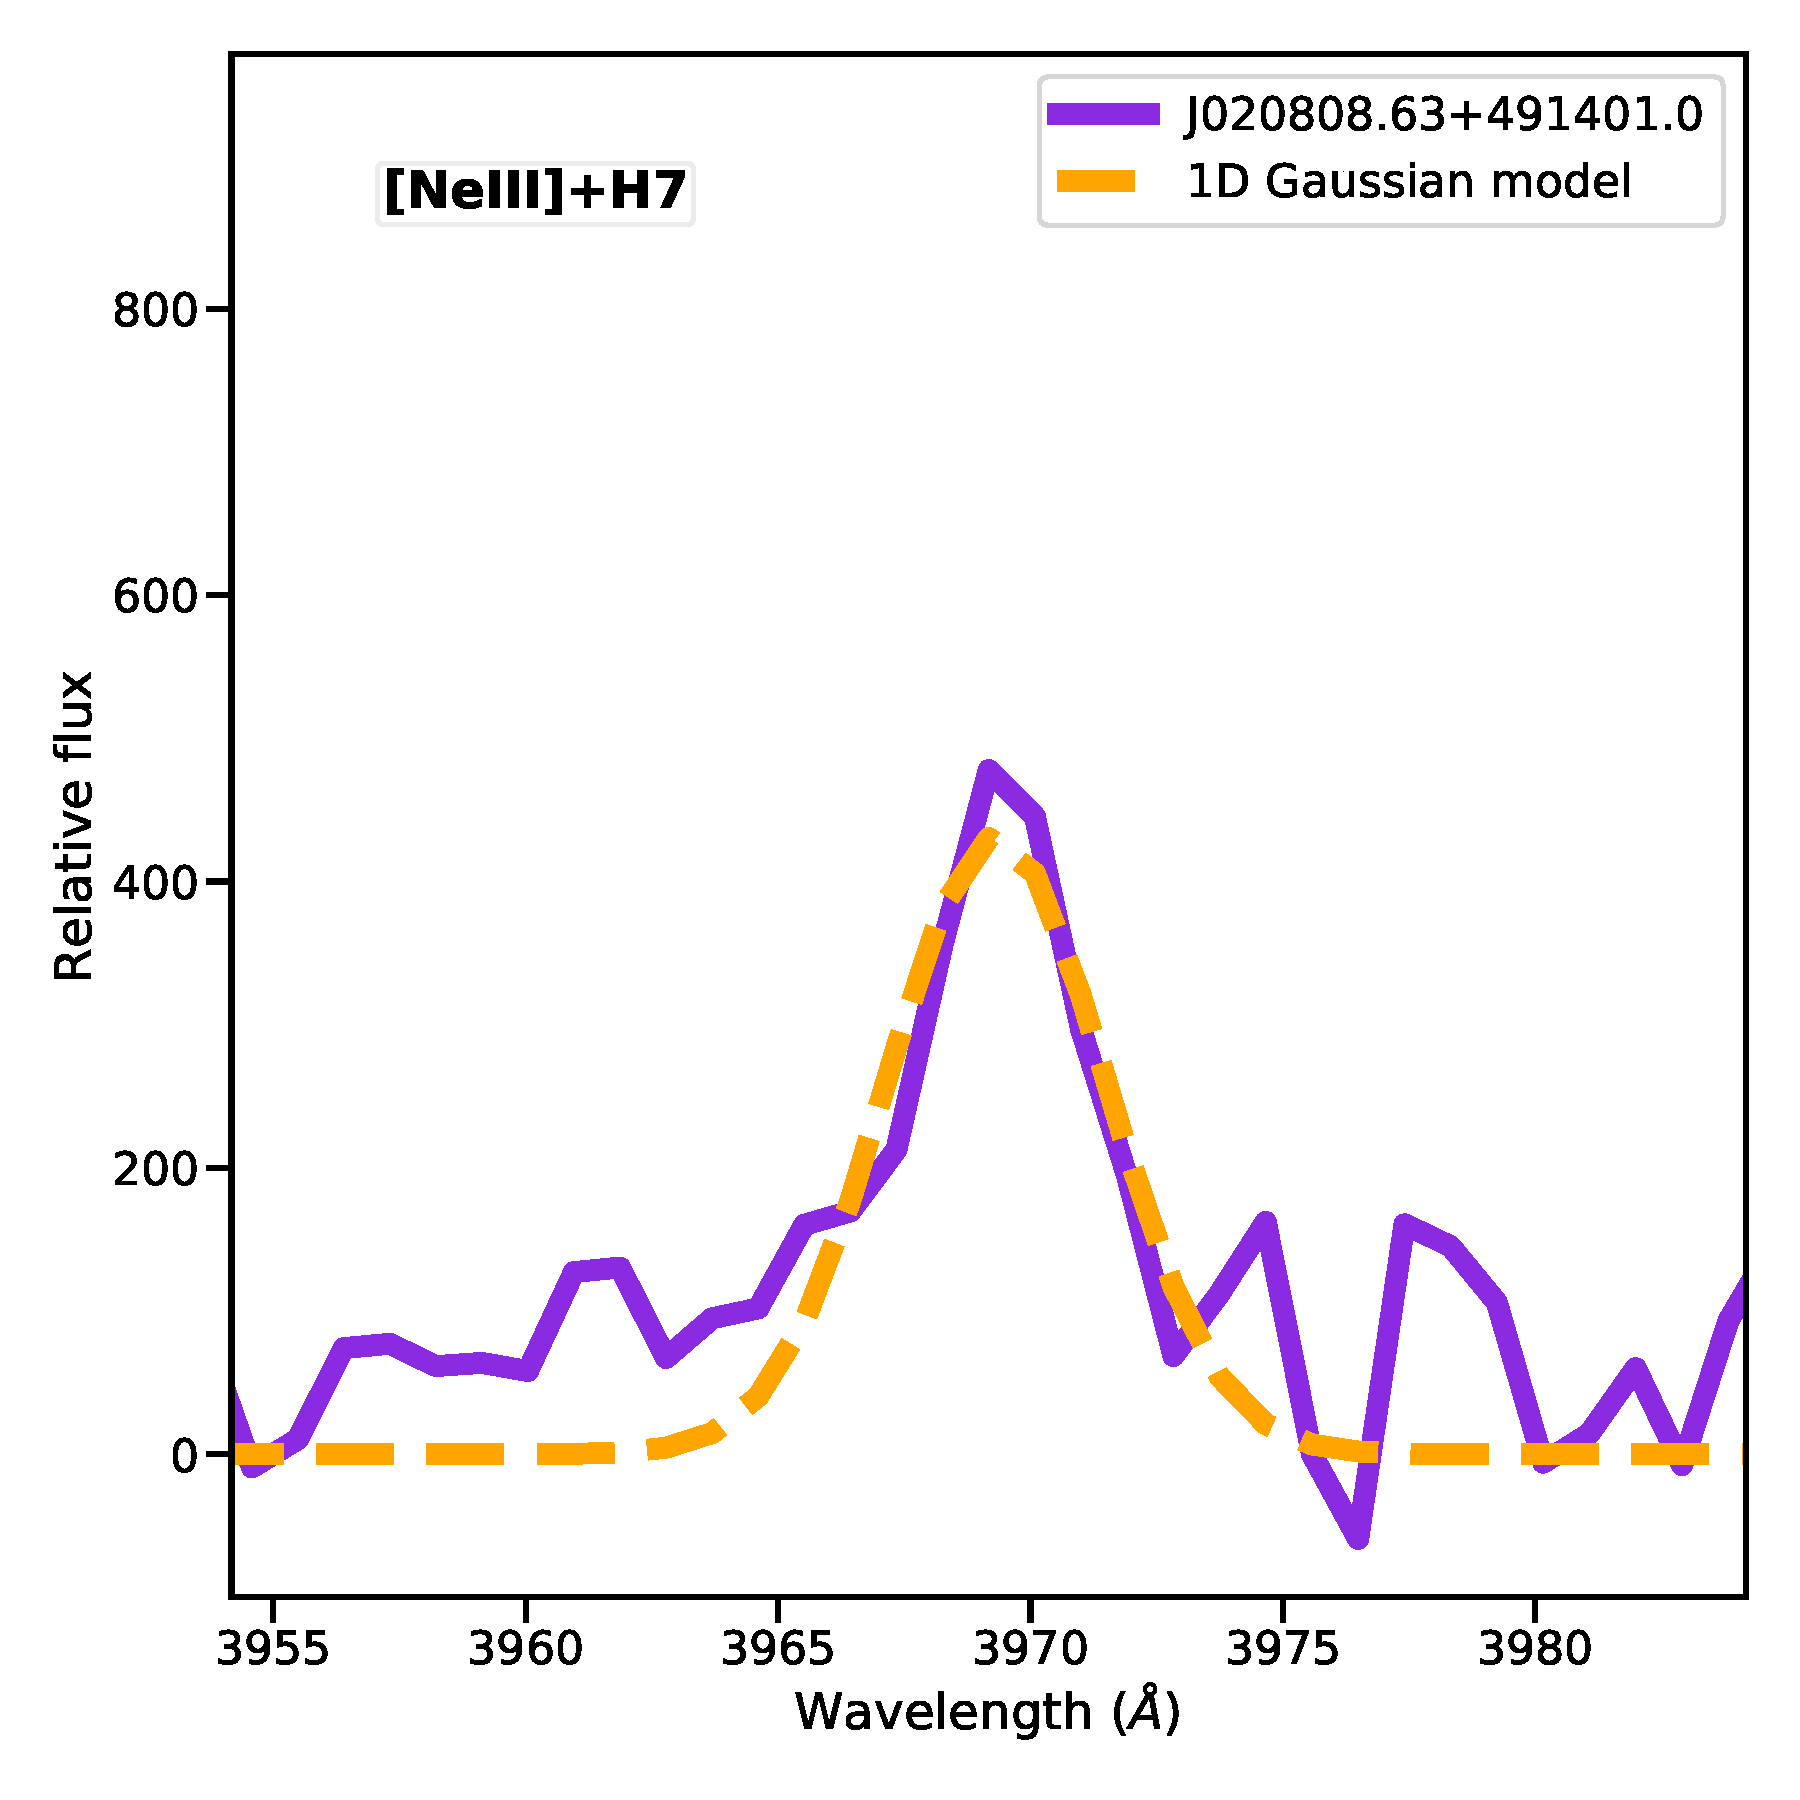
\includegraphics[width=0.3\linewidth, clip]{Figs/Obs_[NeIII]+H7.pdf} & 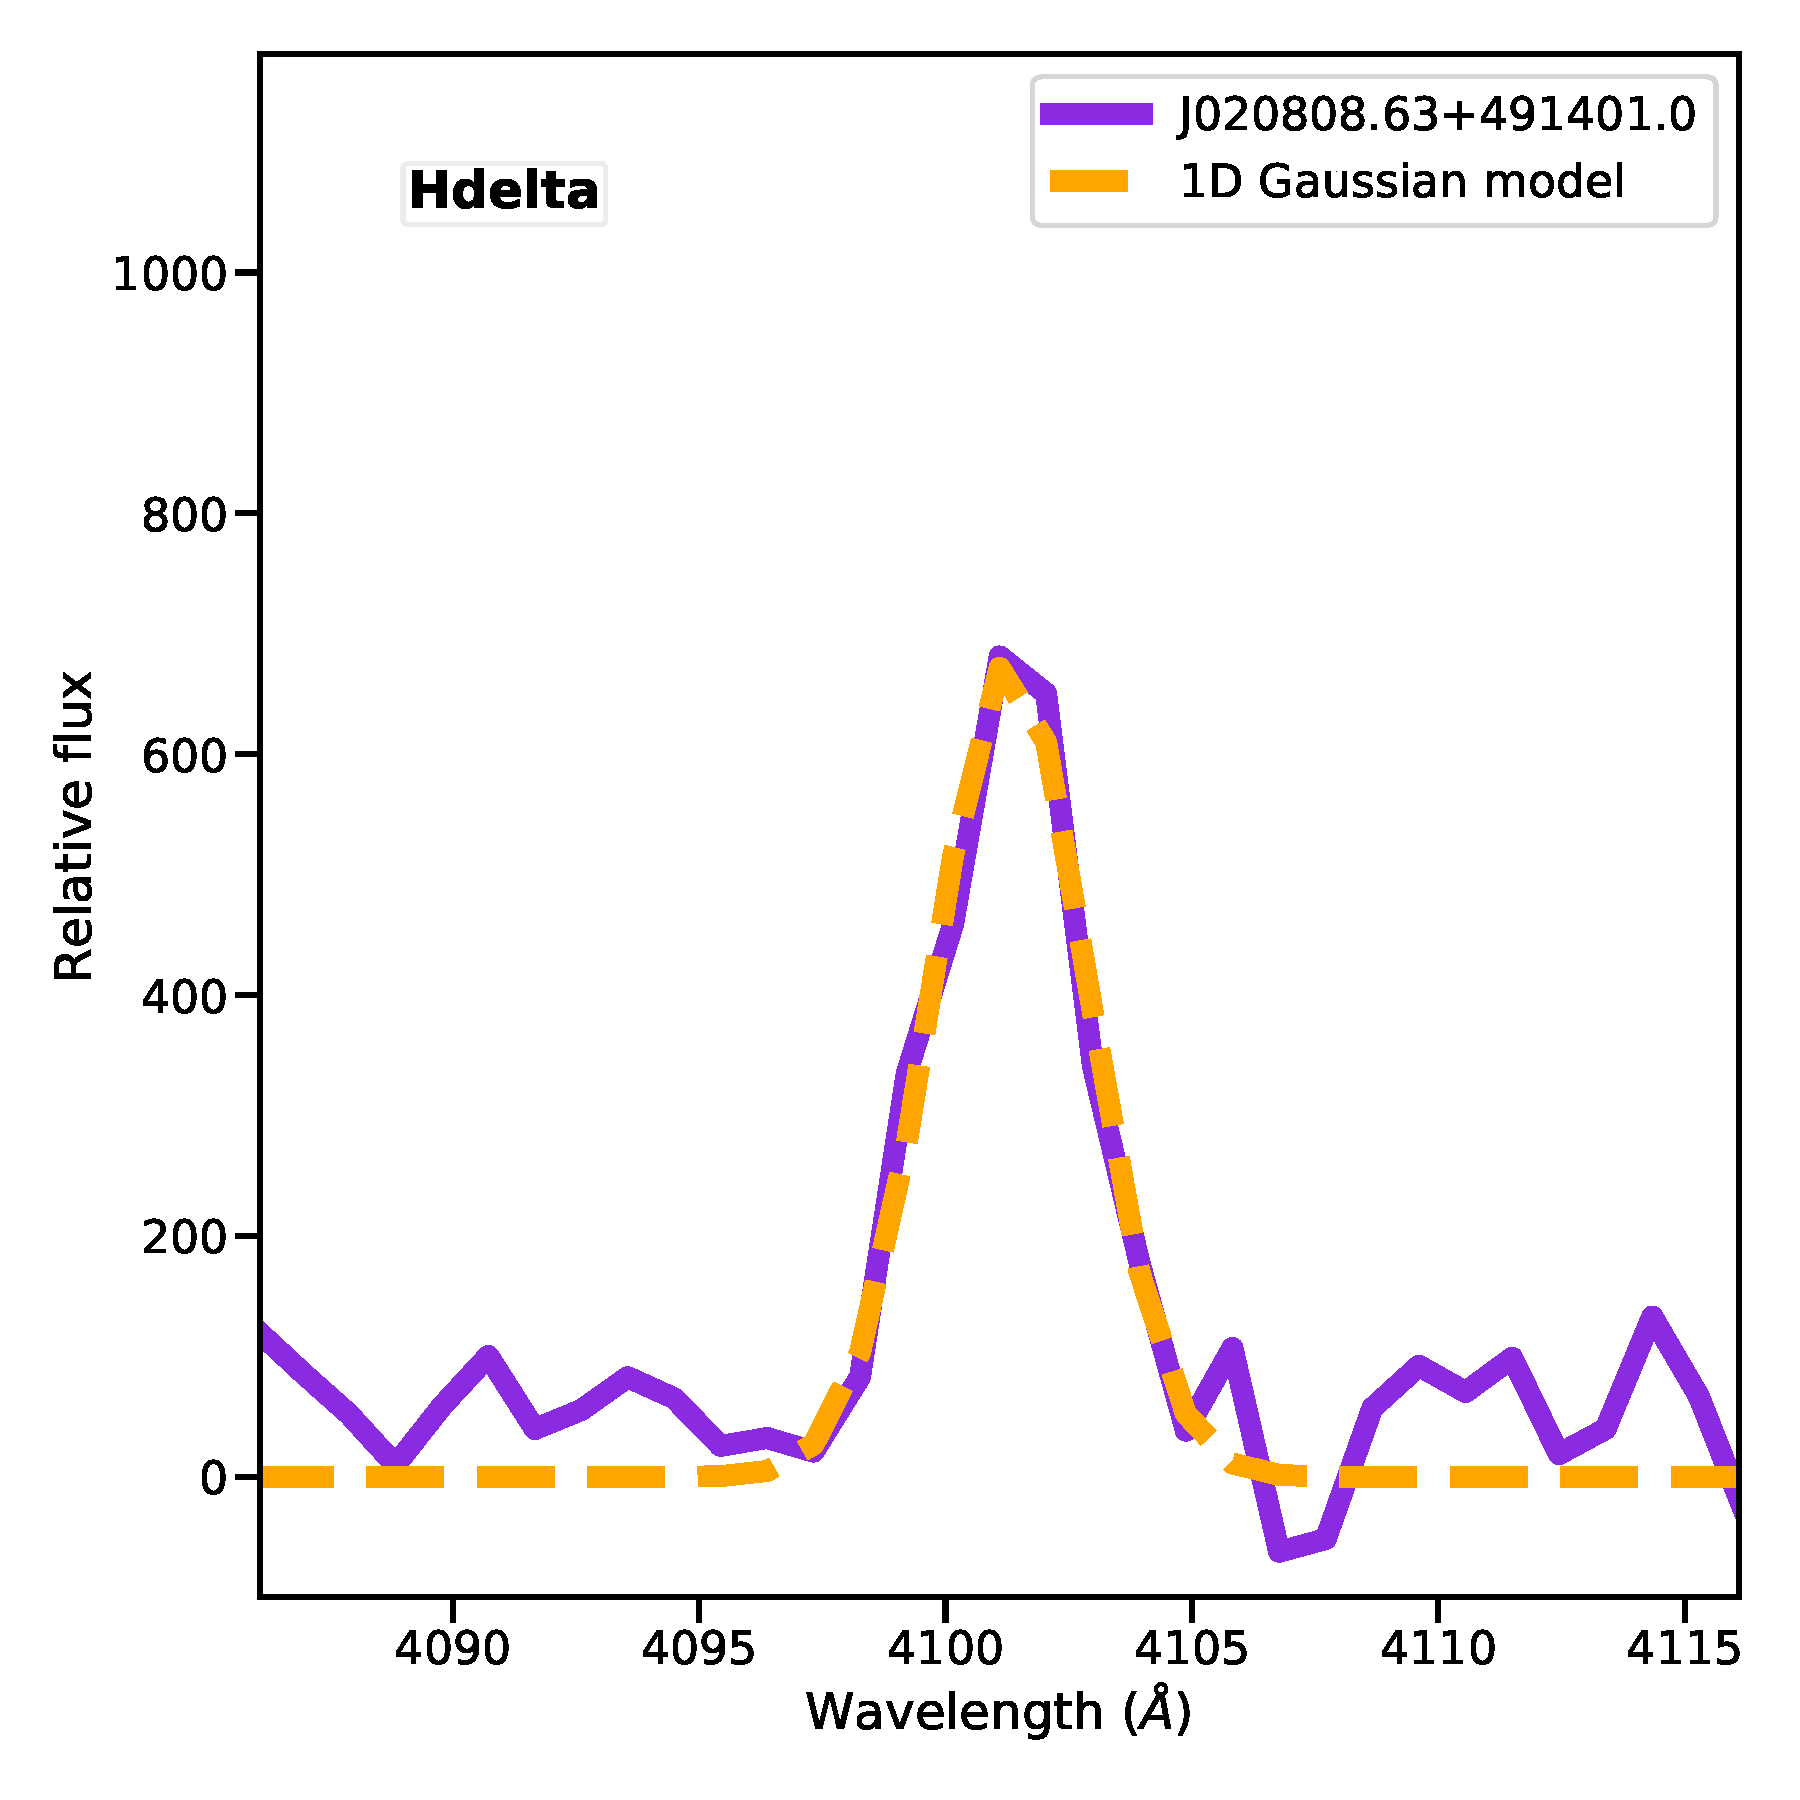
\includegraphics[width=0.3\linewidth, clip]{Figs/Obs_Hdelta.pdf} & 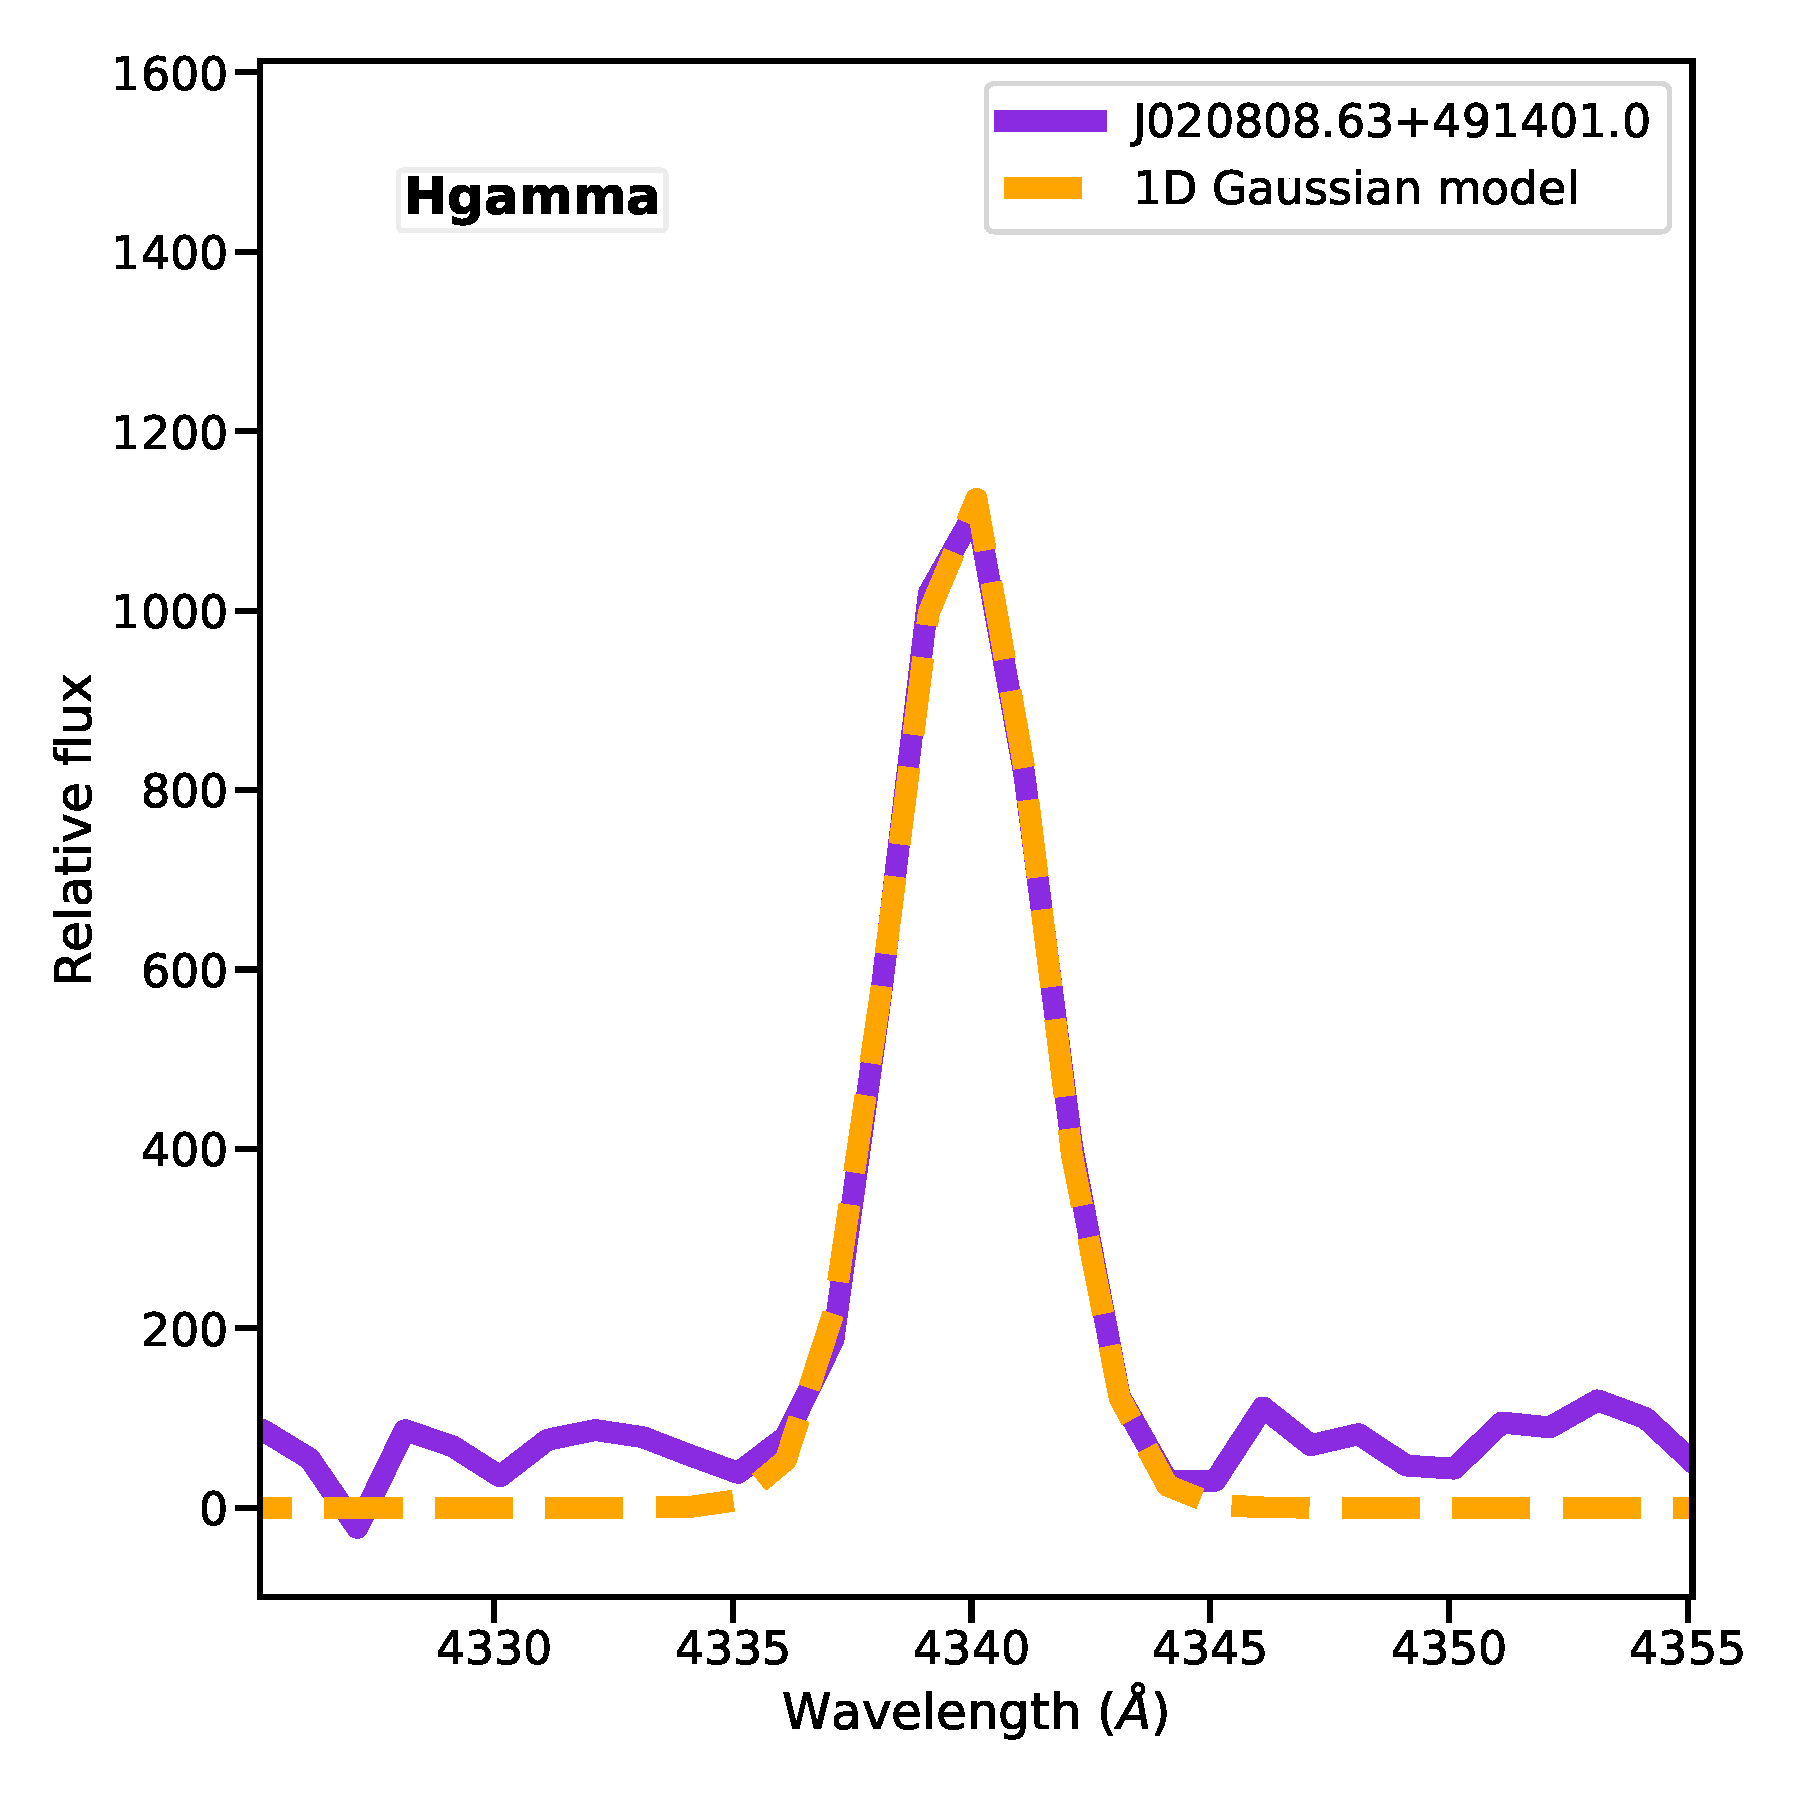
\includegraphics[width=0.3\linewidth, clip]{Figs/Obs_Hgamma.pdf} \\ 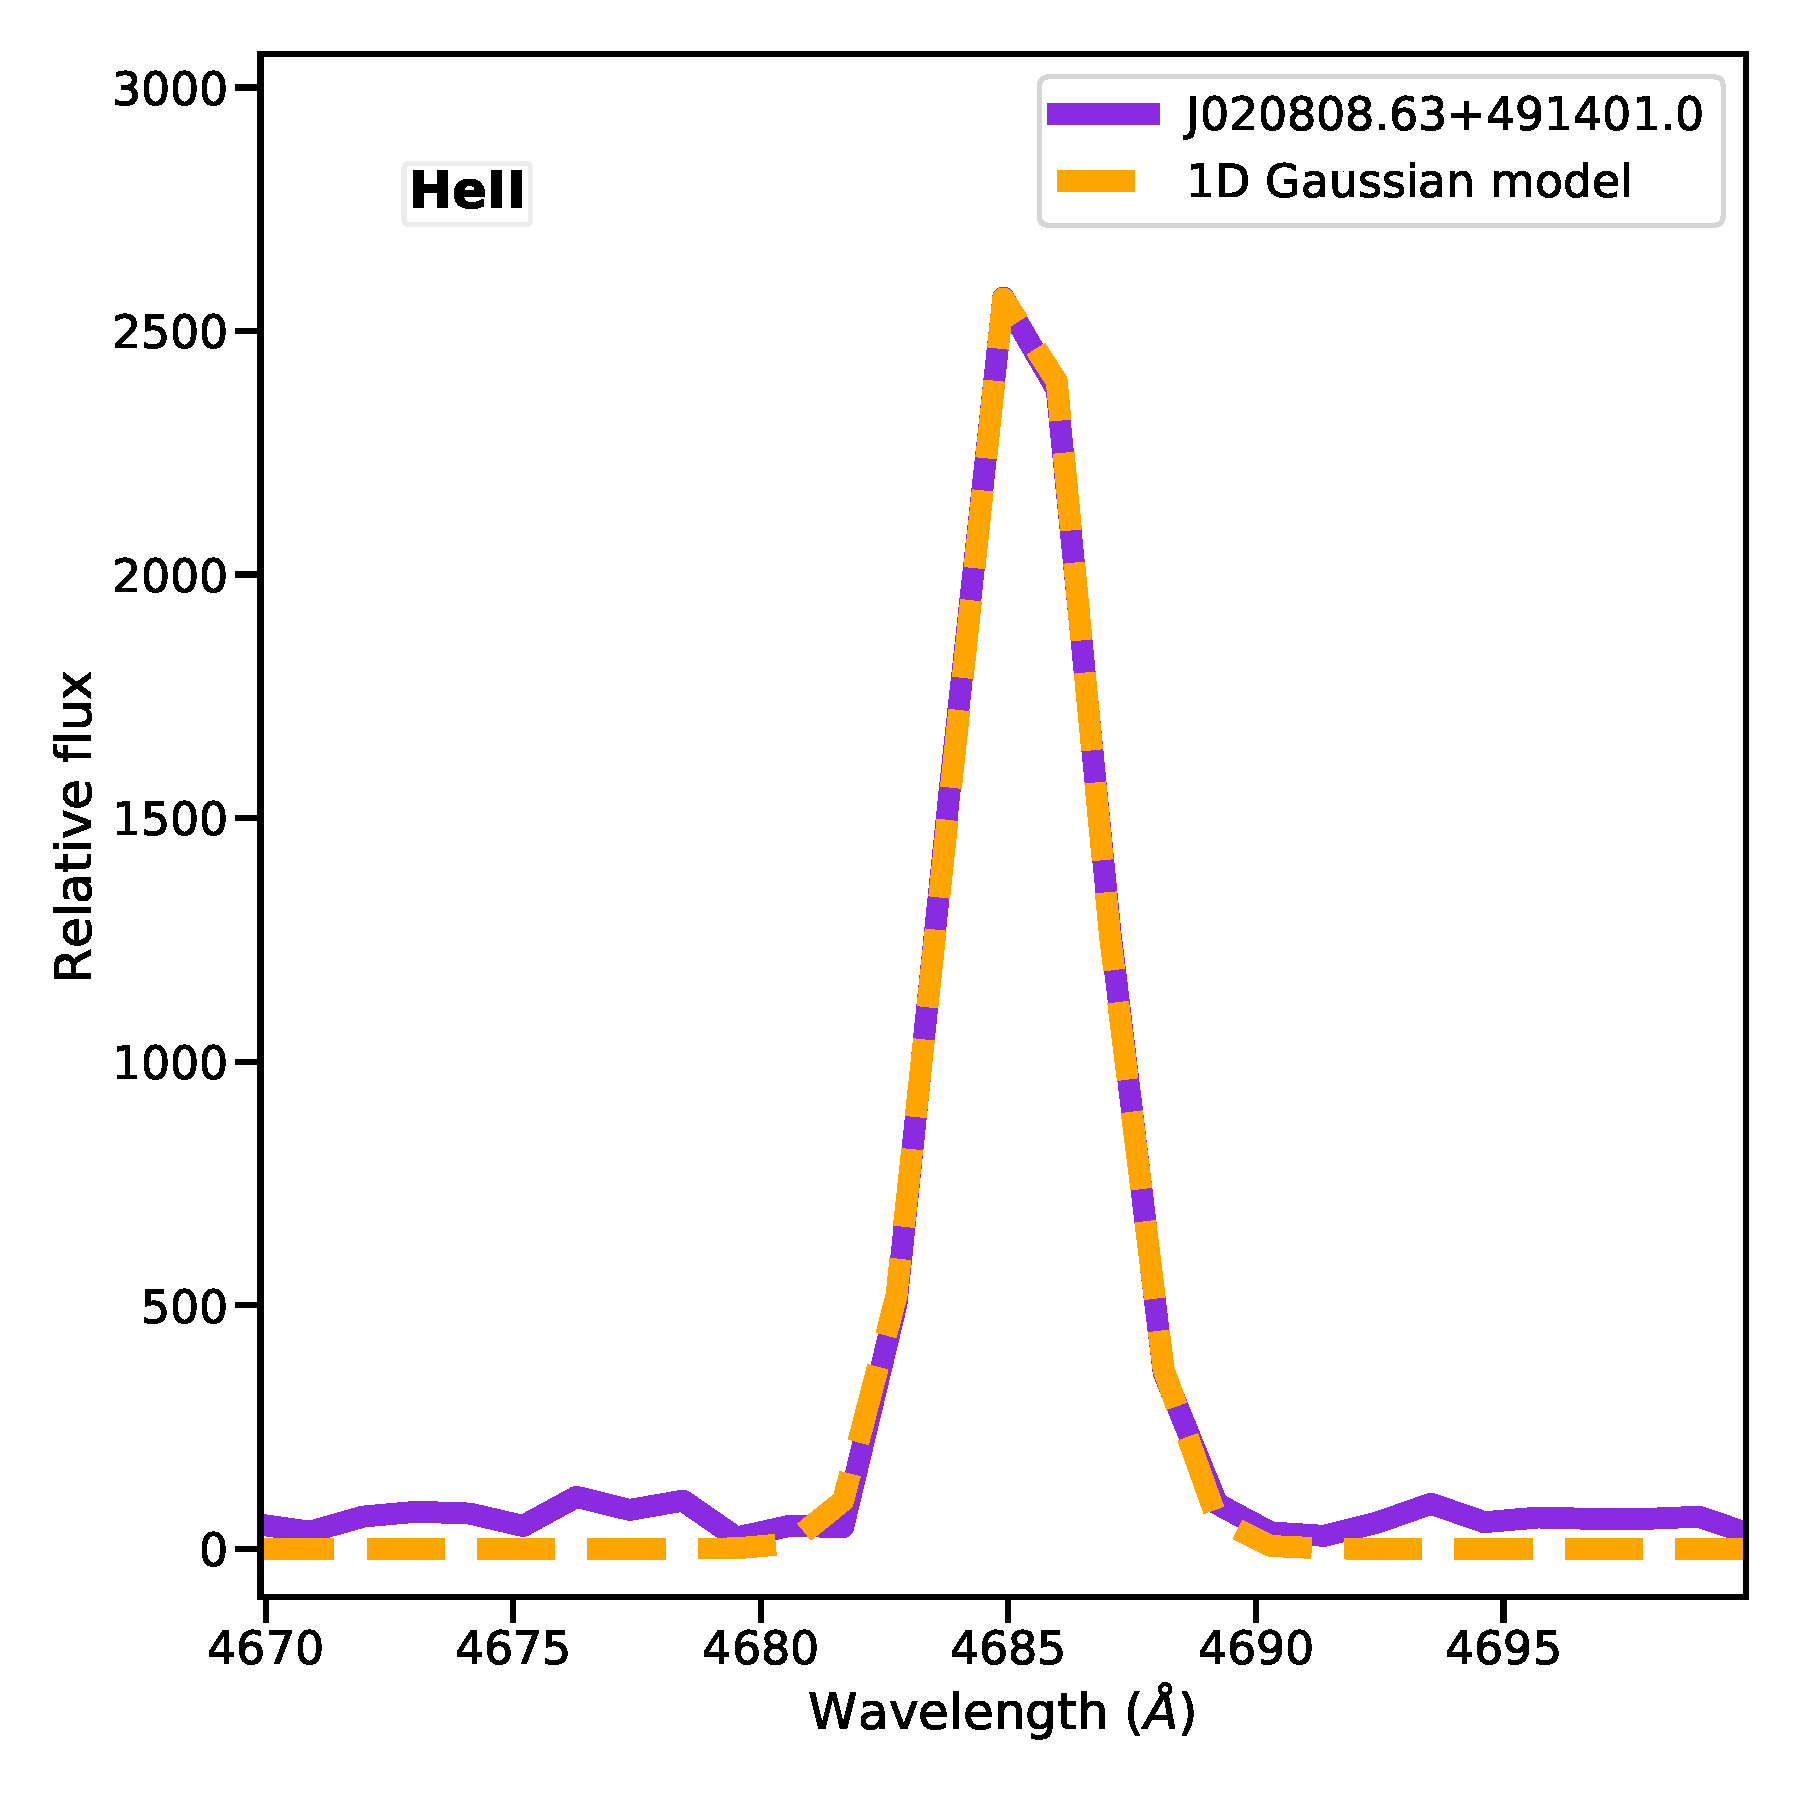
\includegraphics[width=0.3\linewidth, clip]{Figs/Obs_HeII.pdf} &
    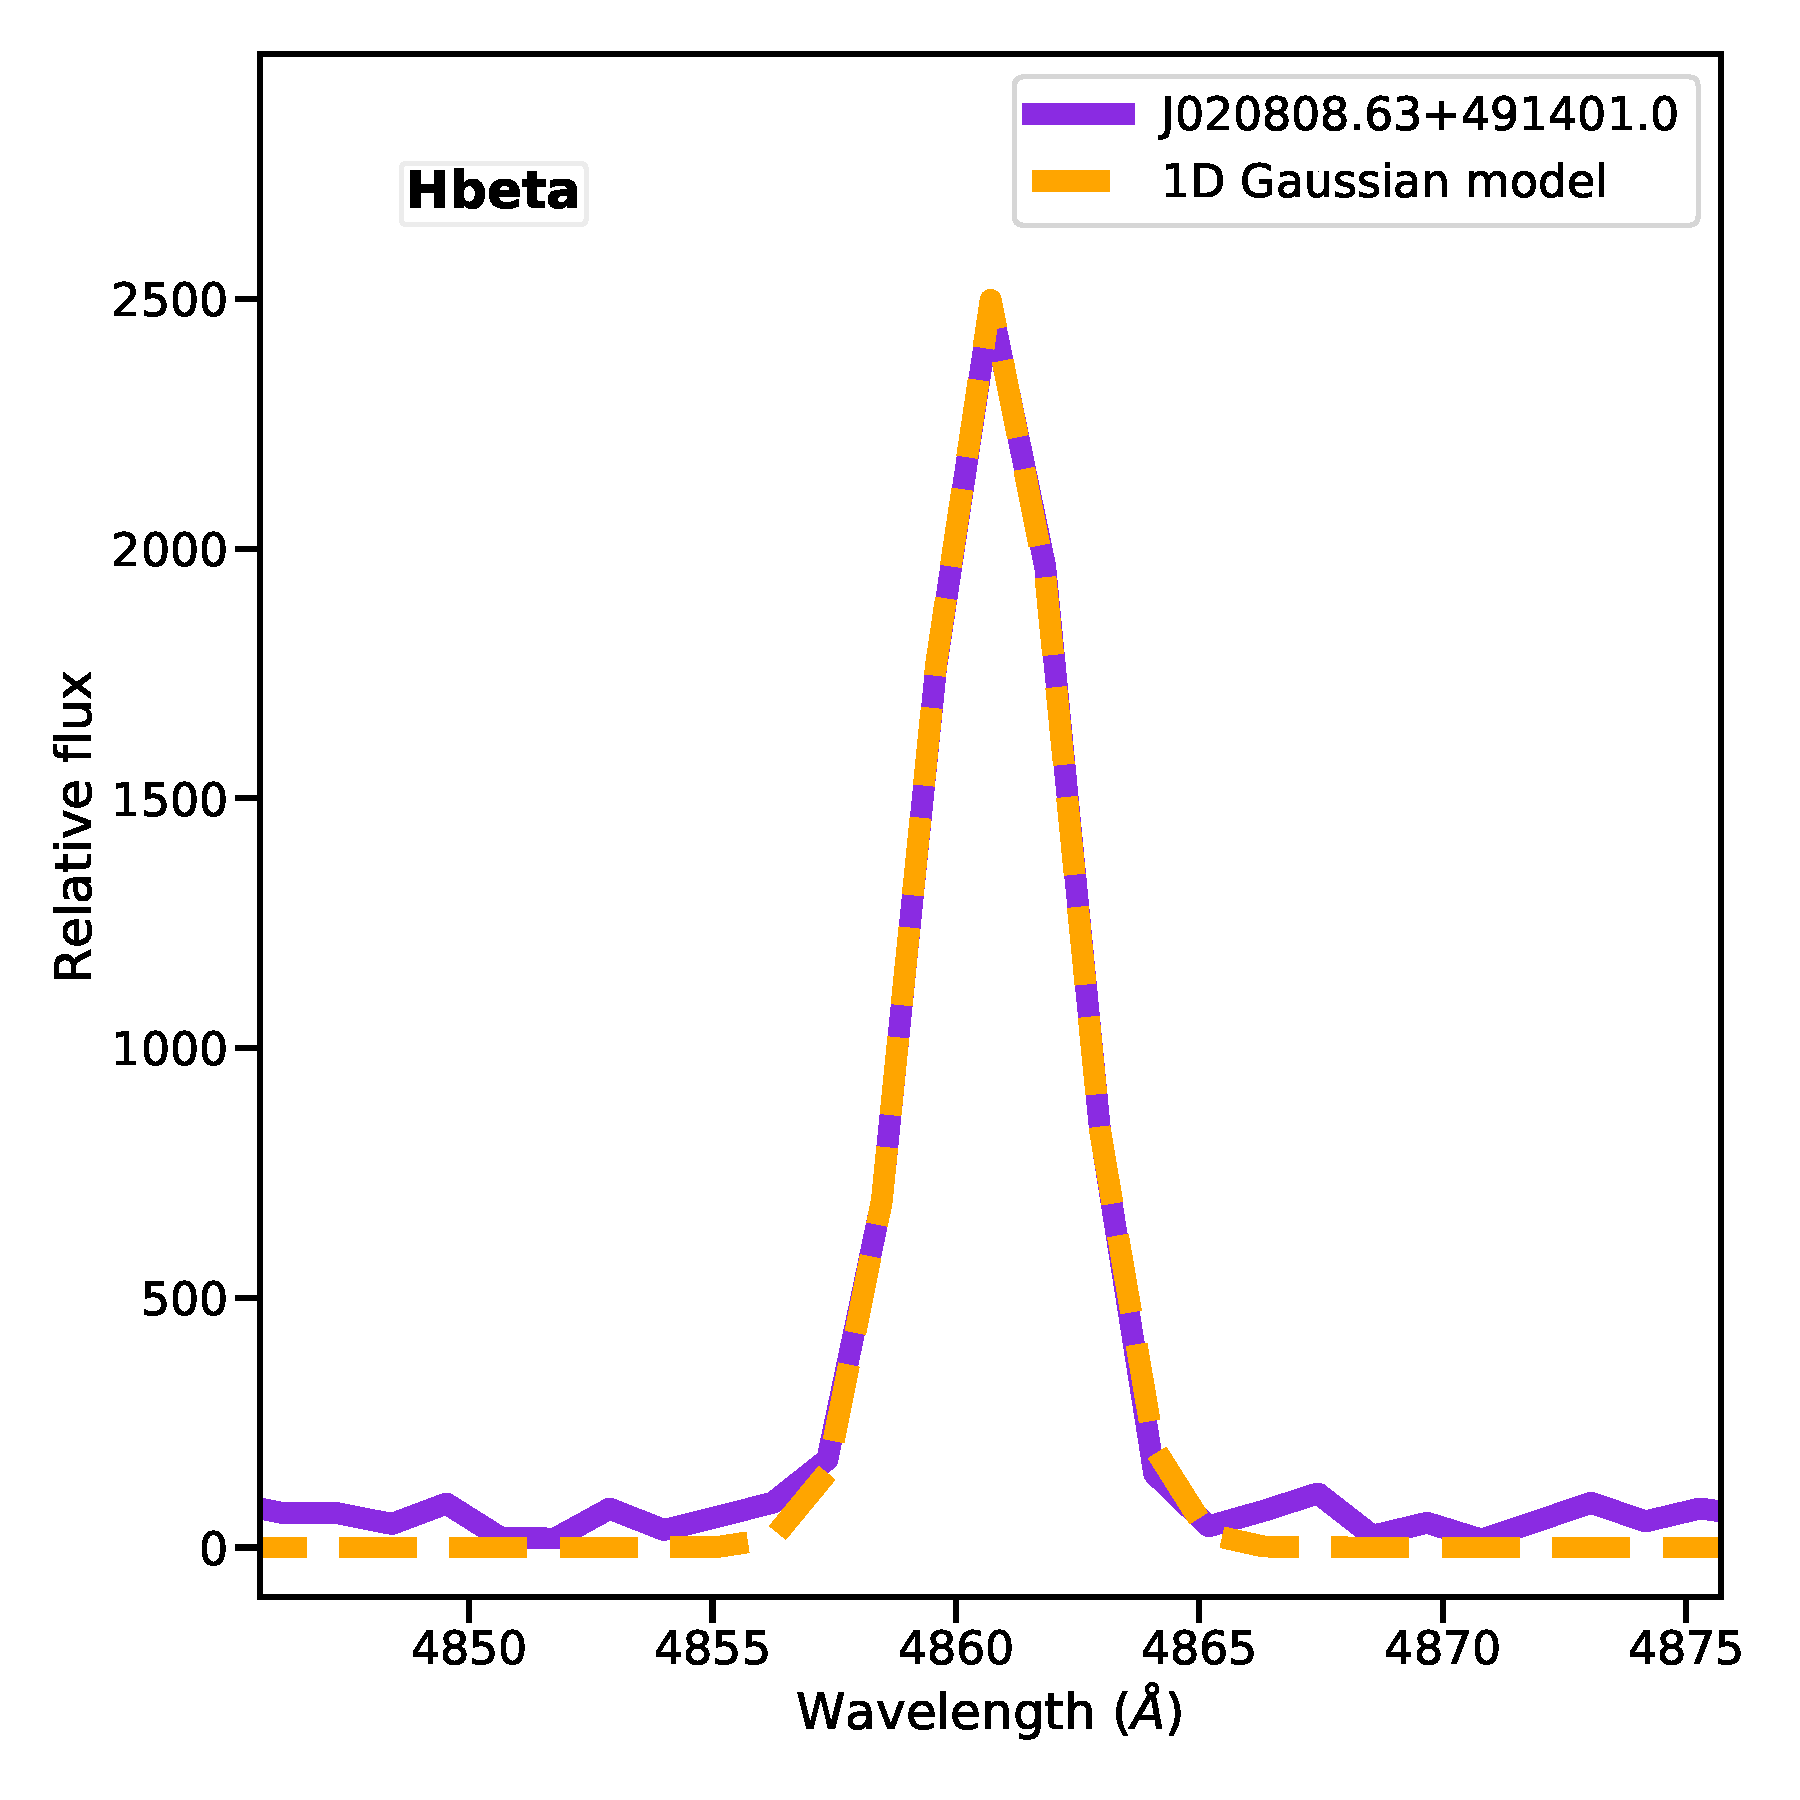
\includegraphics[width=0.3\linewidth, clip]{Figs/Obs_Hbeta.pdf} & 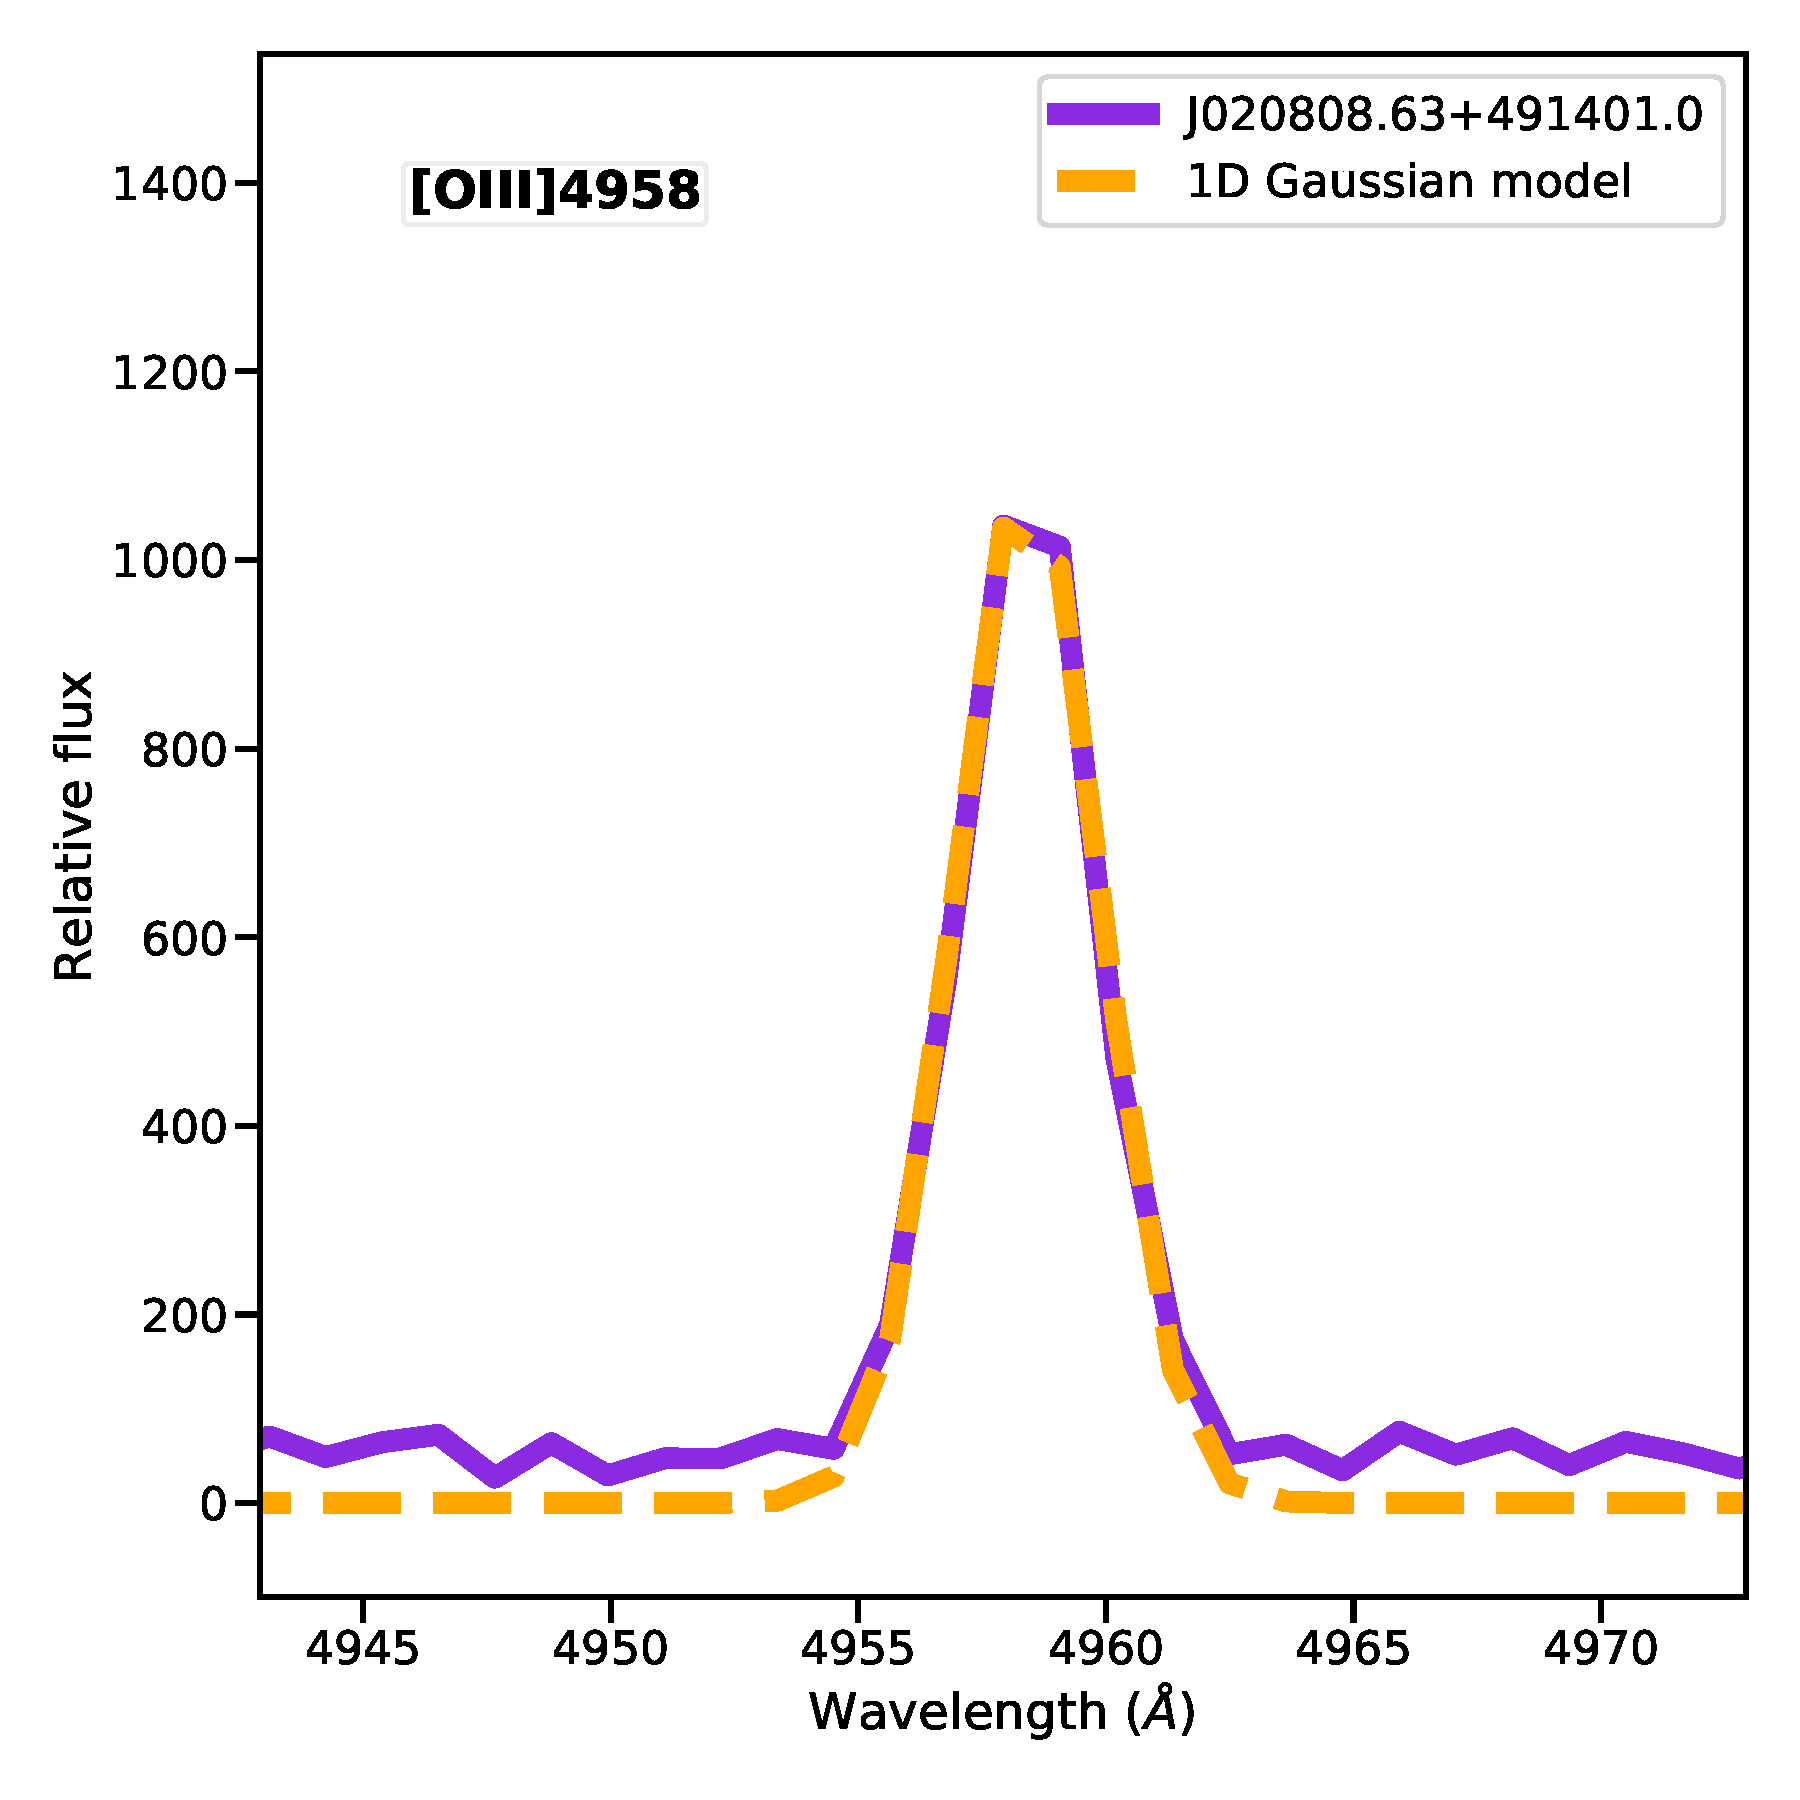
\includegraphics[width=0.3\linewidth, clip]{Figs/Obs_[OIII]4958.pdf} \\ 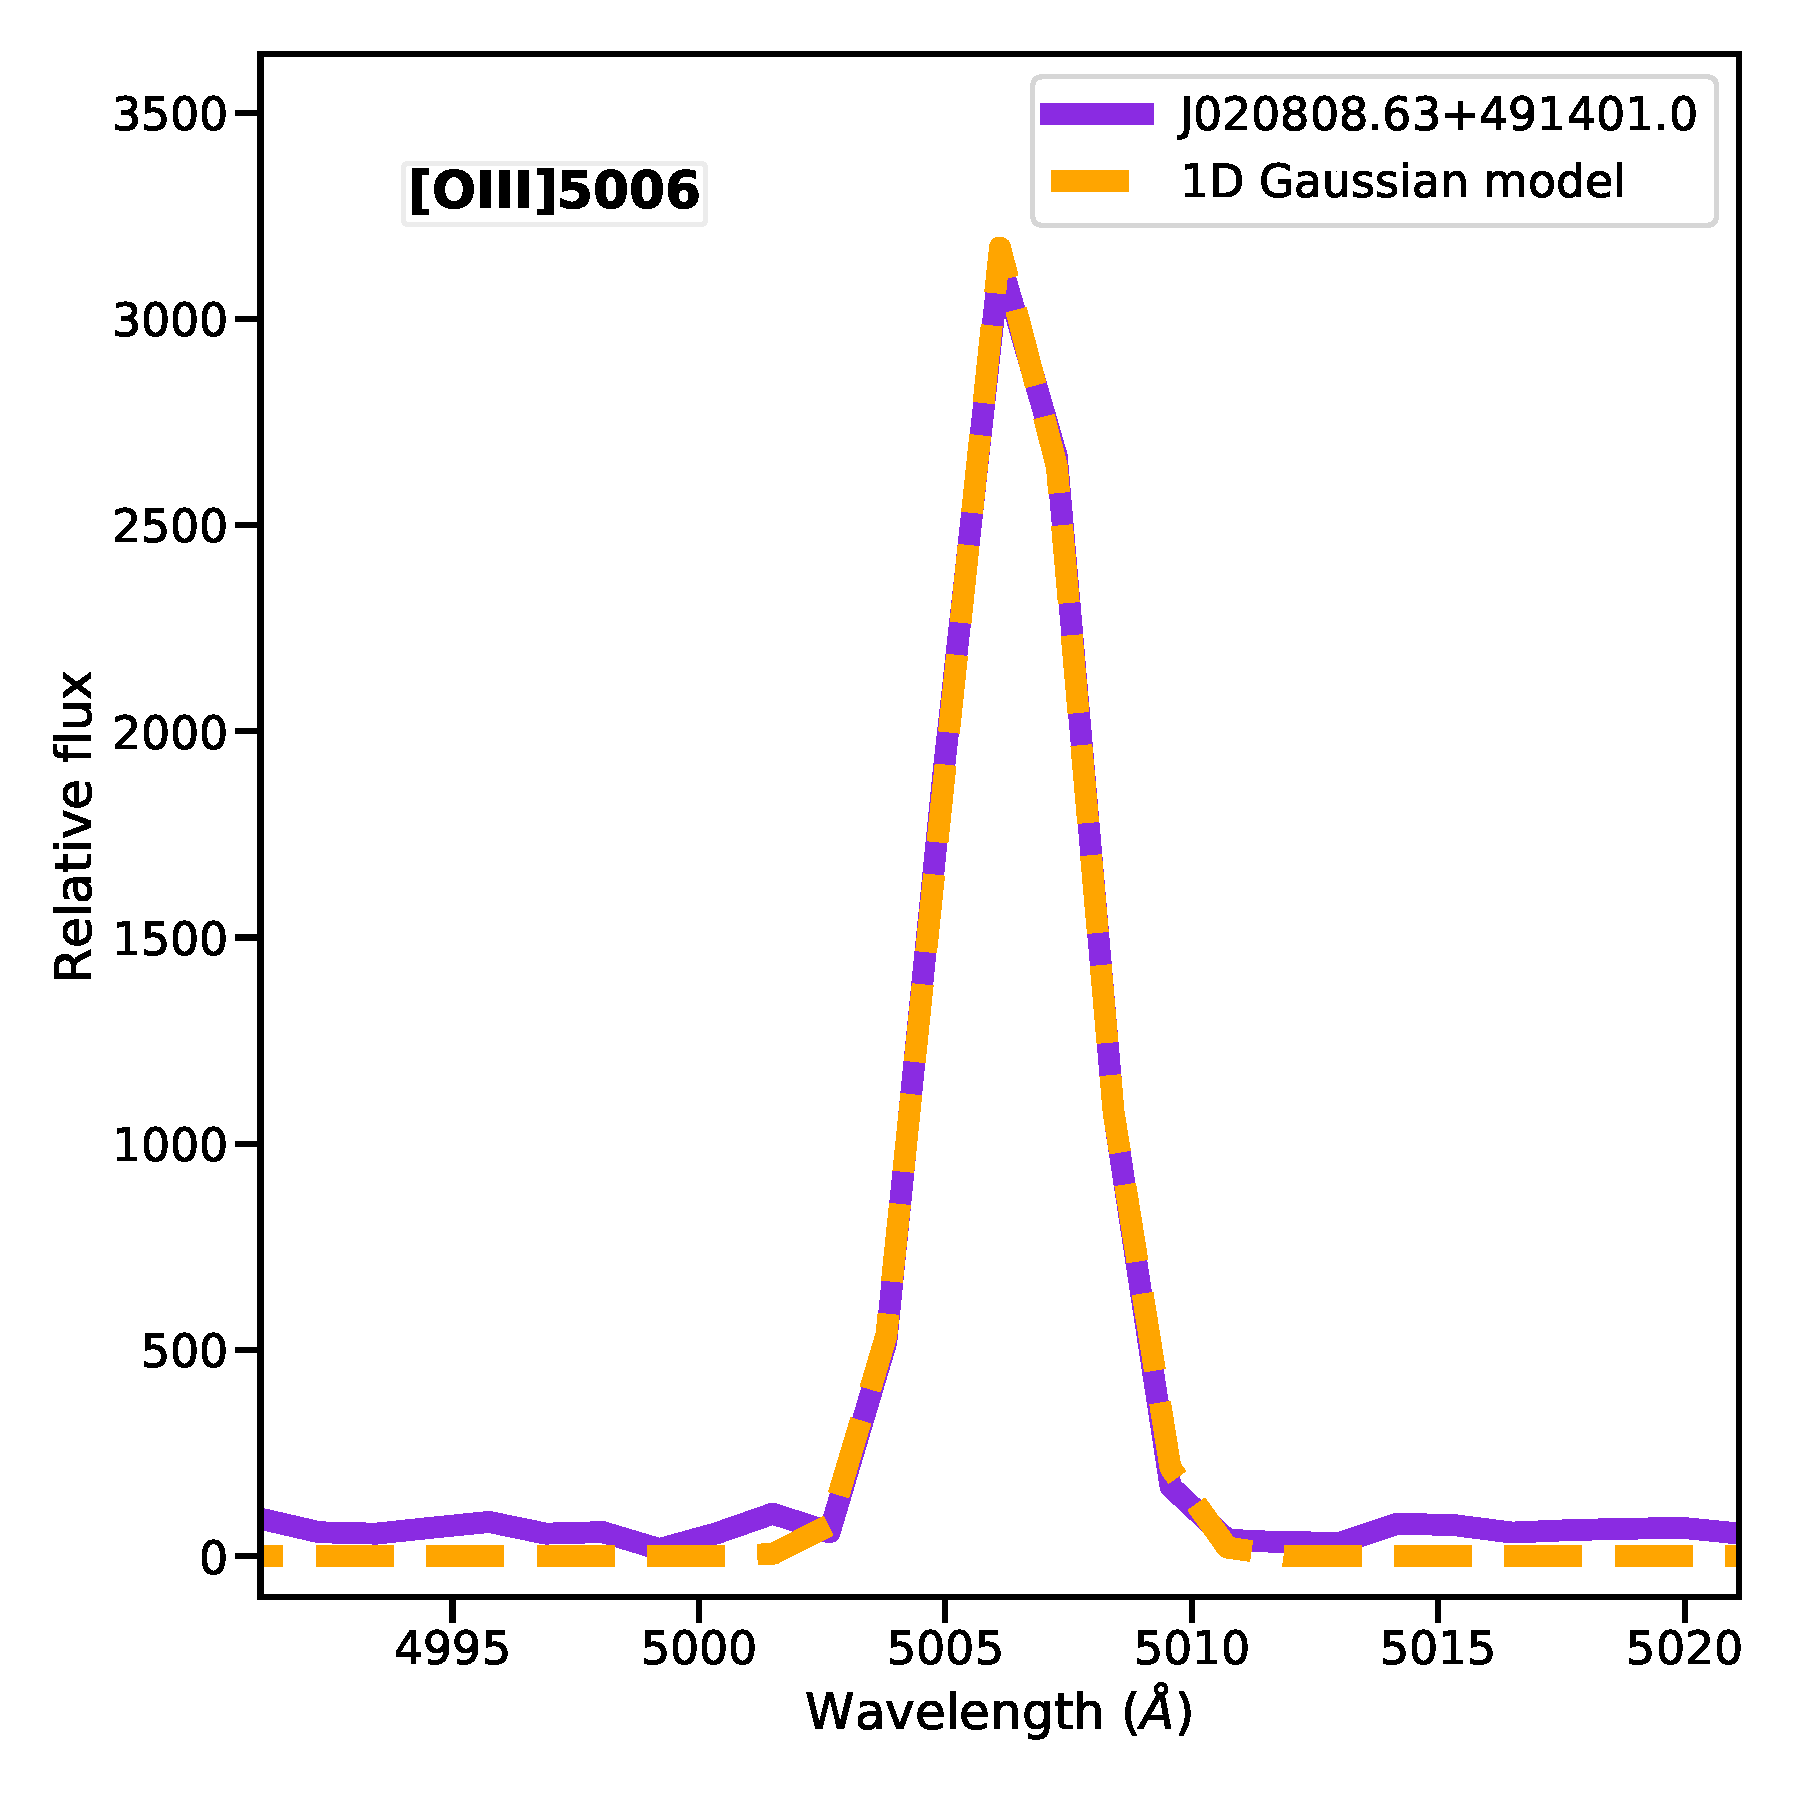
\includegraphics[width=0.3\linewidth, clip]{Figs/Obs_[OIII]5006.pdf} & 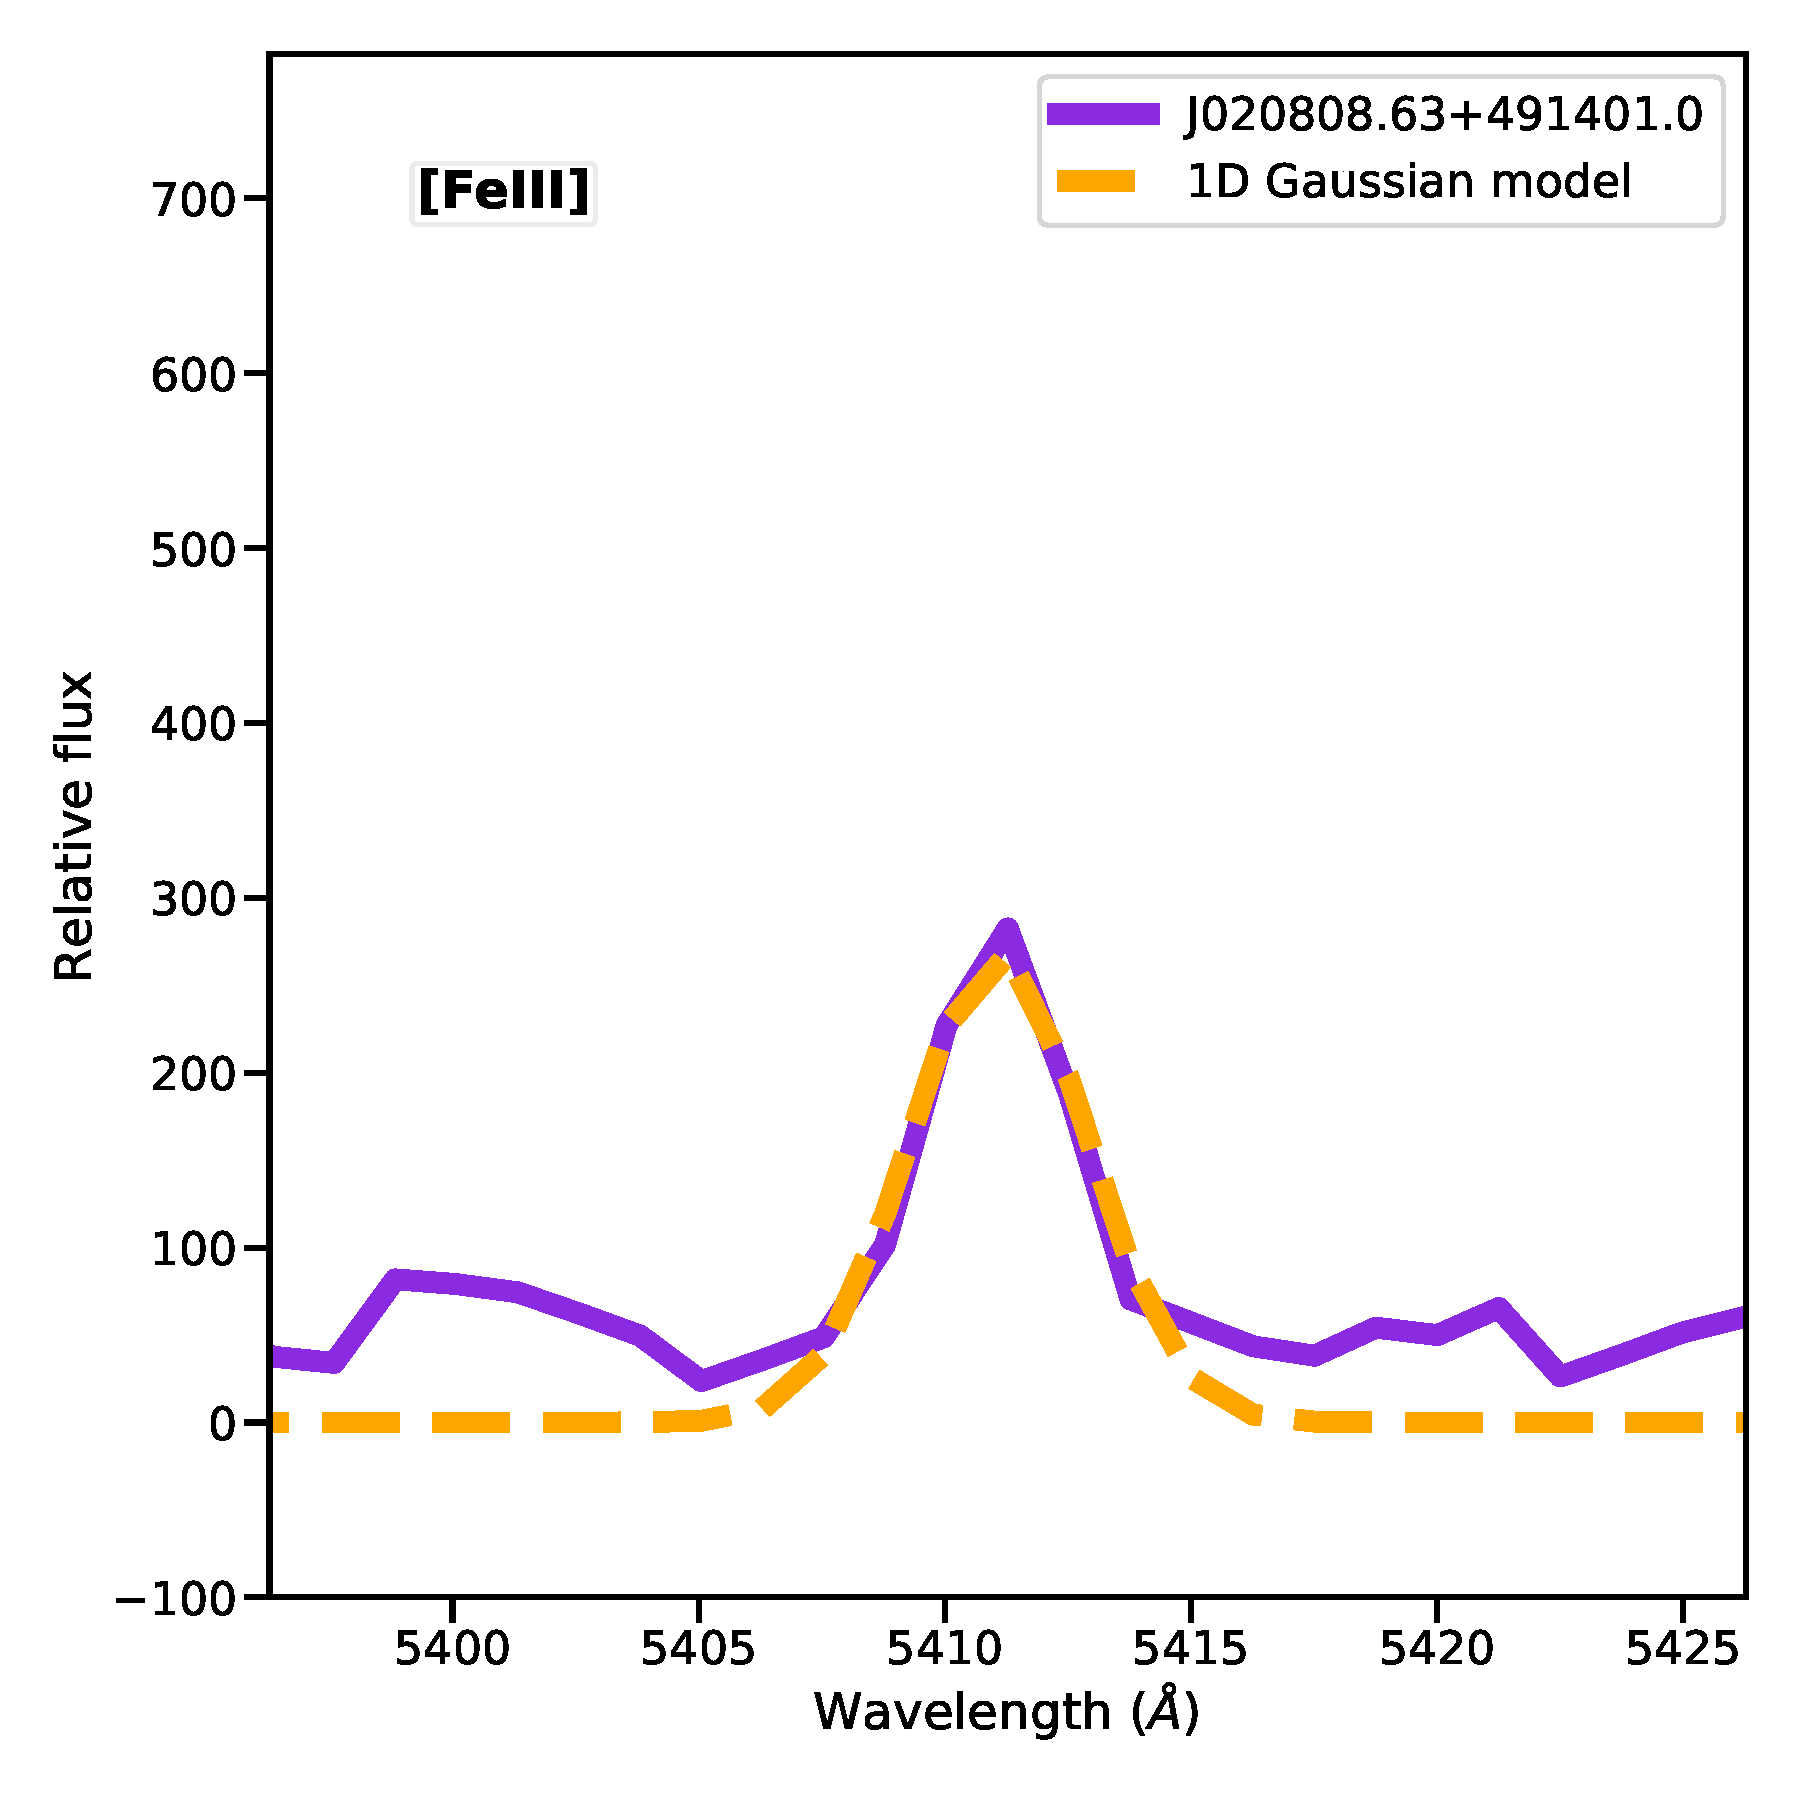
\includegraphics[width=0.3\linewidth, clip]{Figs/Obs_[FeIII].pdf} &
    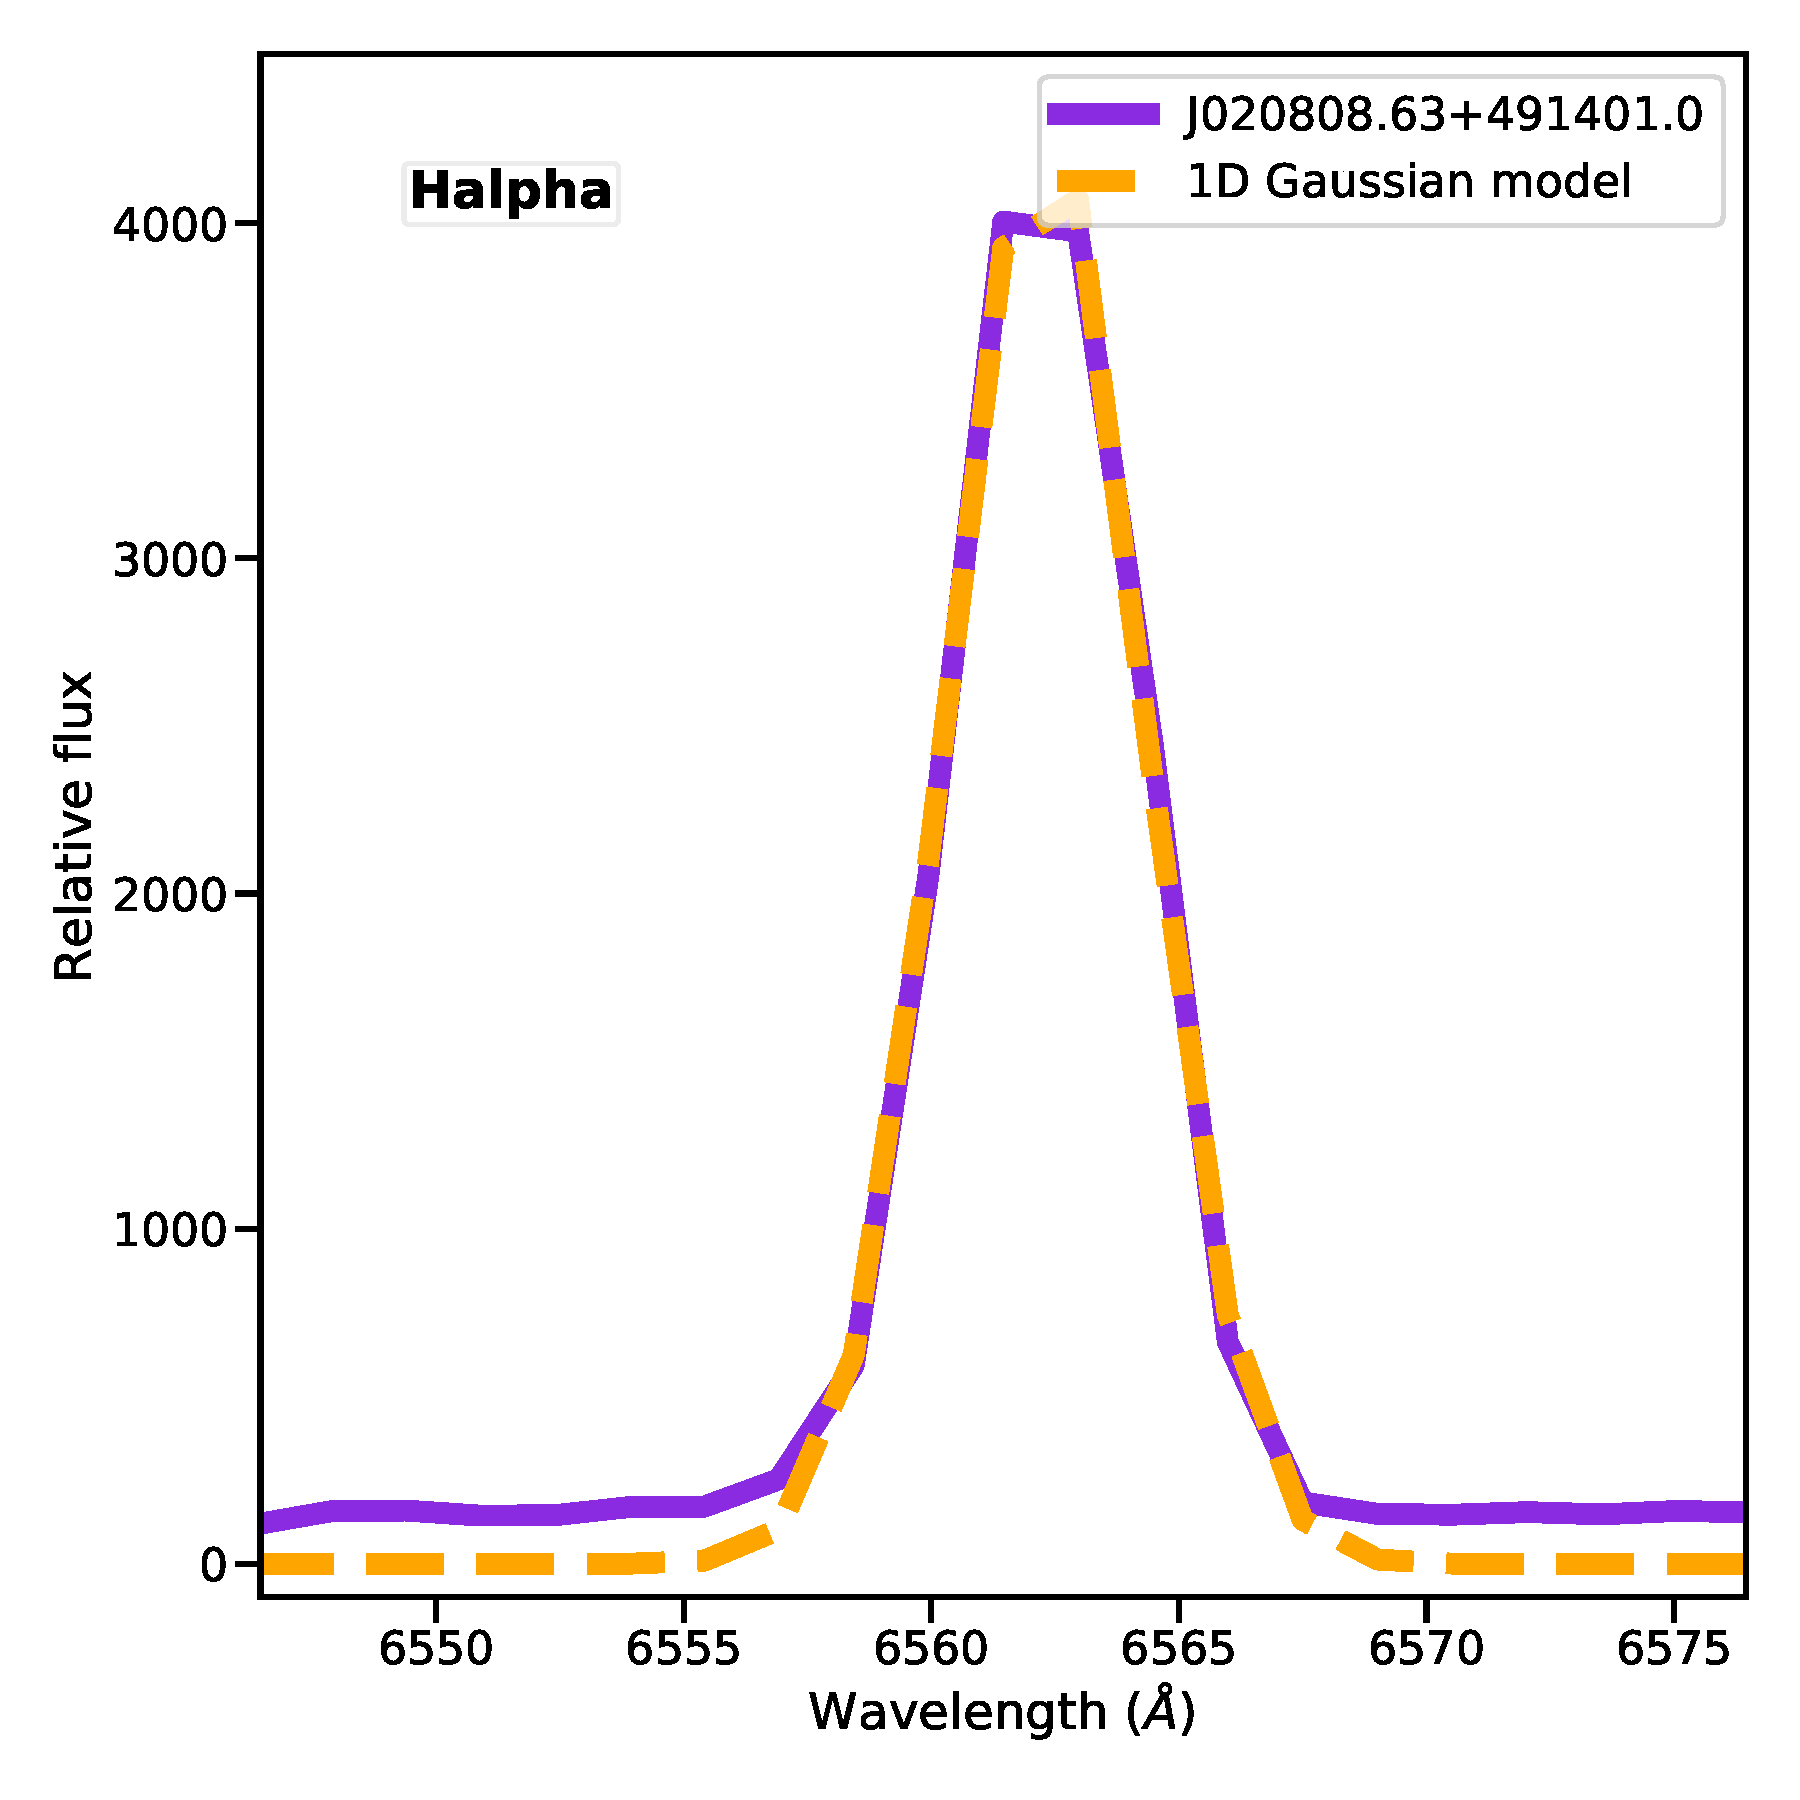
\includegraphics[width=0.3\linewidth, clip]{Figs/Obs_Halpha.pdf} \\
\end{tabular}
\end{table*}

%% \section{The best fitted models}
%% The Fig show the {\sc cloudy} models with value on the $\chi^{2}_r$ between 1 and 2.
%% \begin{table*}
\centering
  \caption{The best fitted models, on which the $\chi^{2}_r$ have value between 1 and 2. \label{tab:best-model12}}\
  \begin{tabular}{l l l l }
    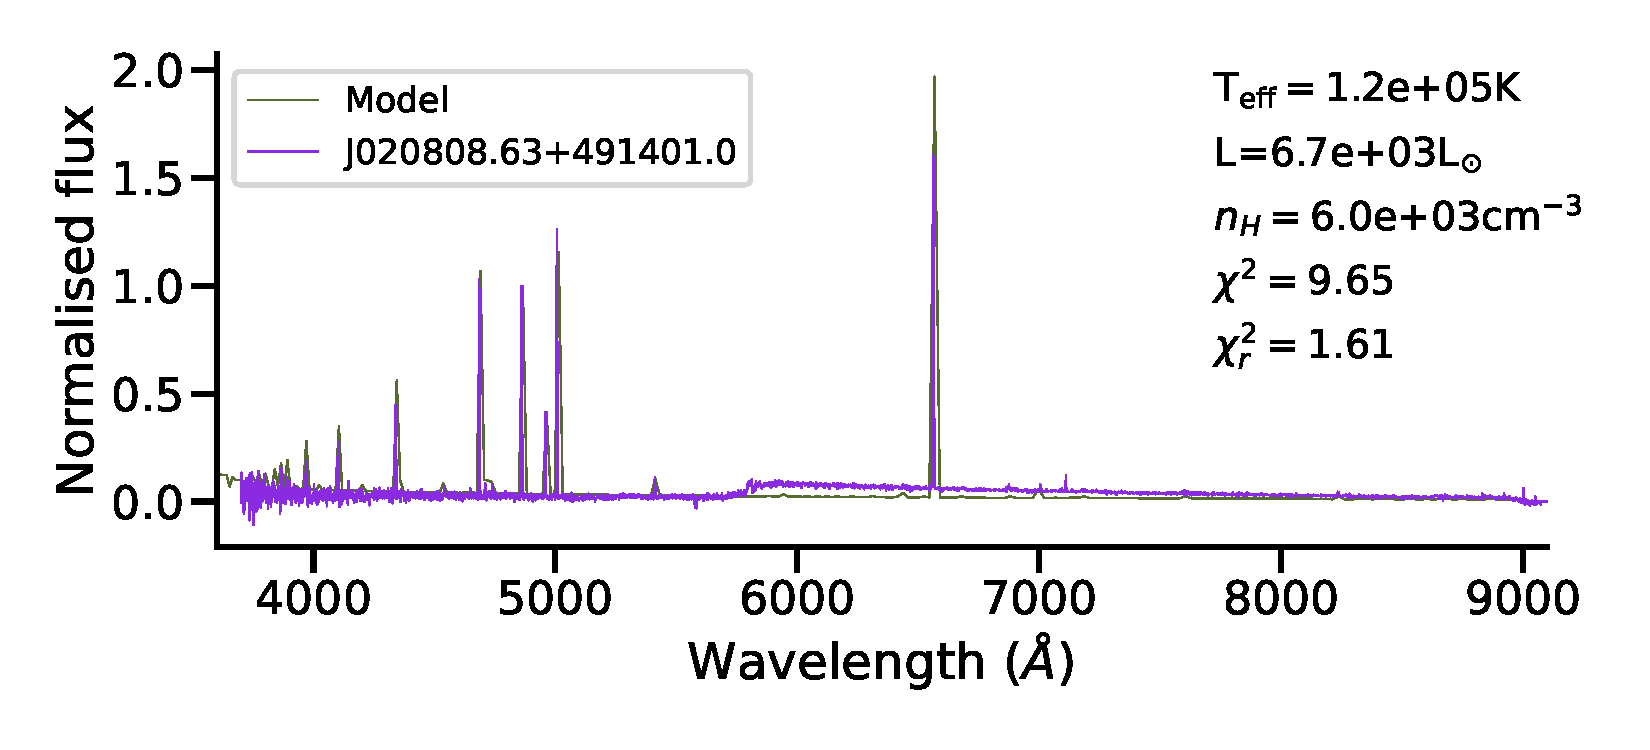
\includegraphics[width=0.24\linewidth, clip]{Figs/model_120000_37.41_3.78.pdf} & 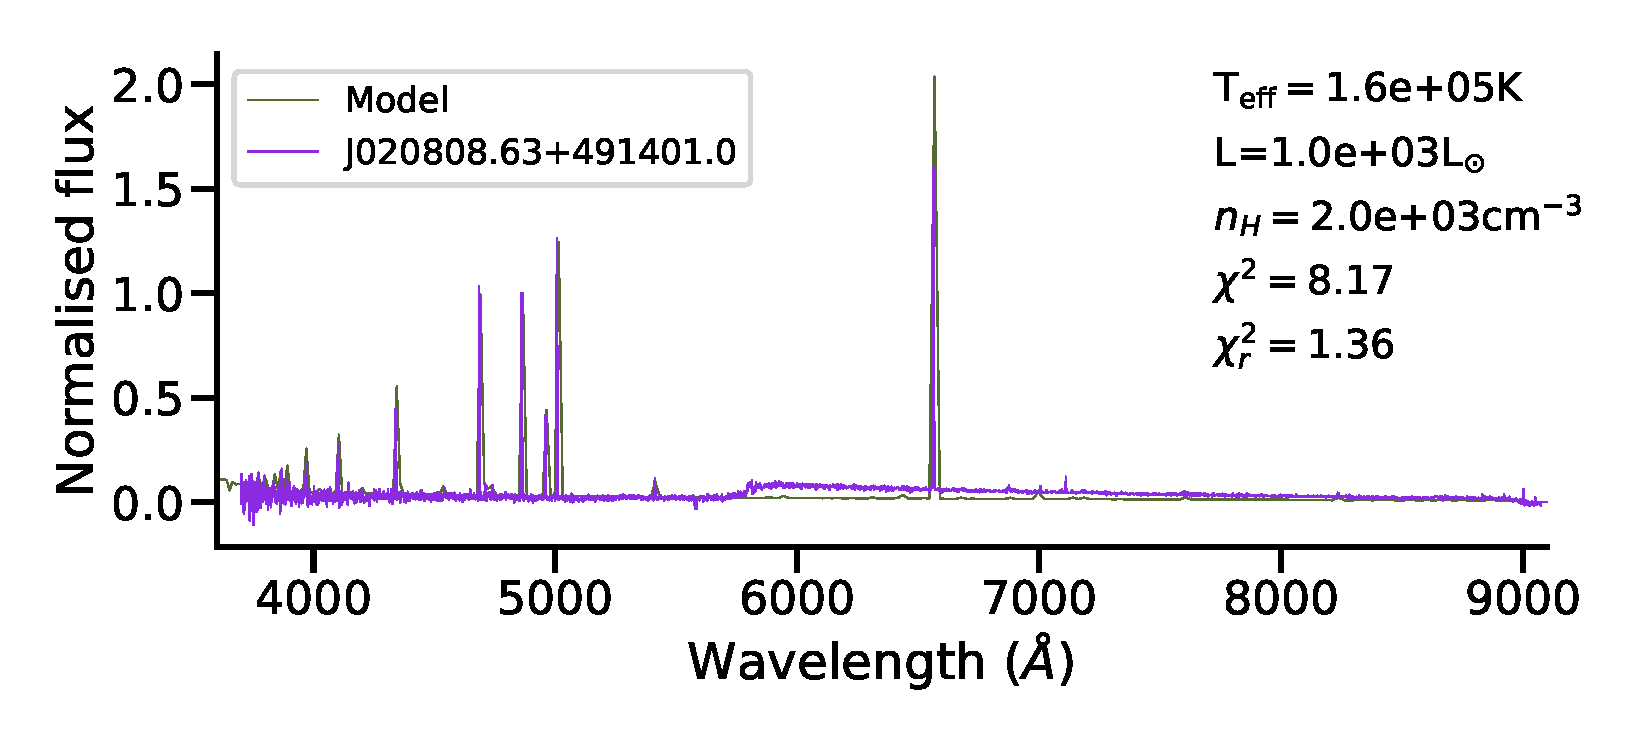
\includegraphics[width=0.24\linewidth, clip]{Figs/model_160000_36.58_3.30.pdf} & 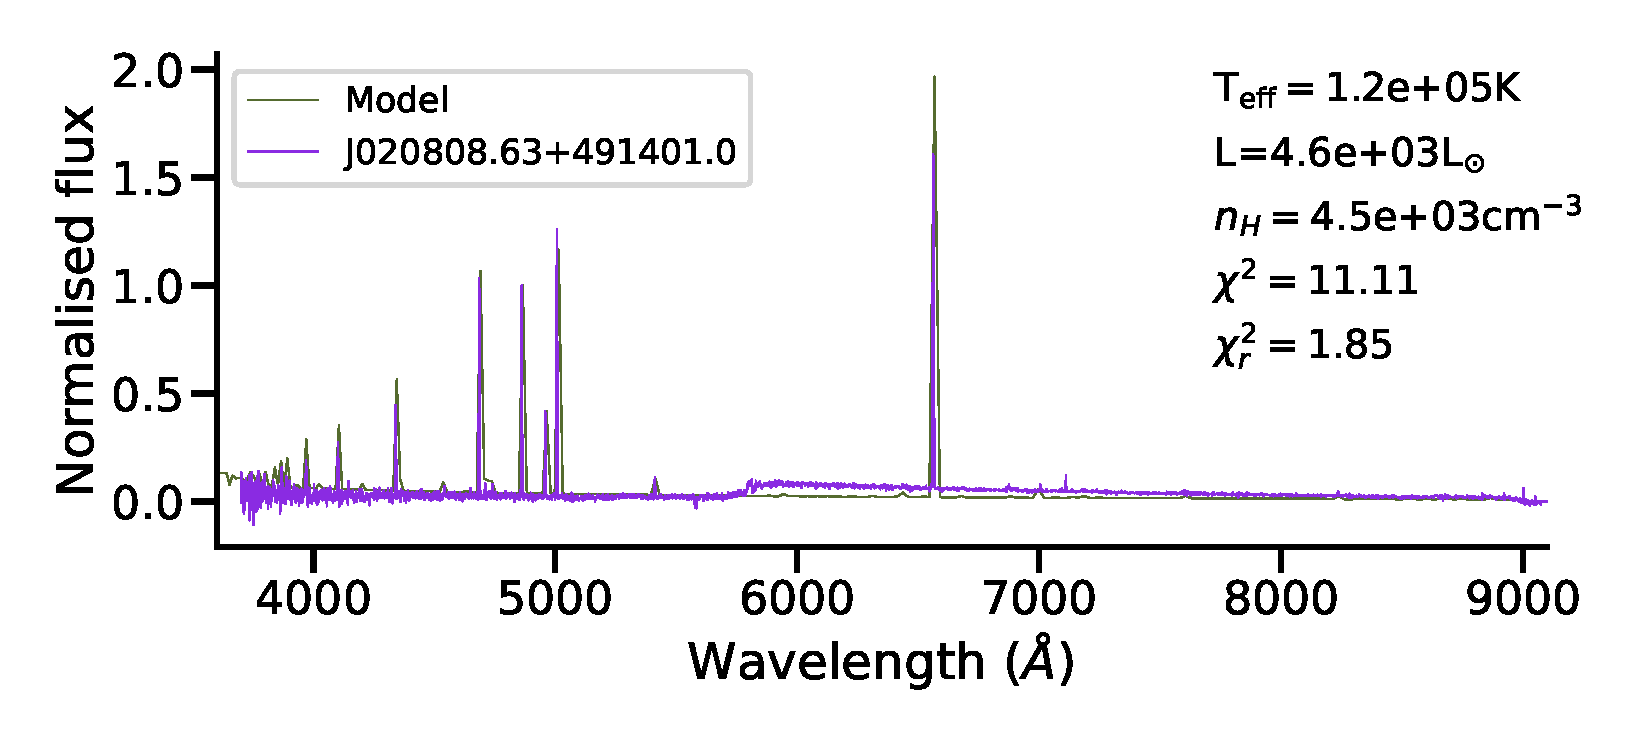
\includegraphics[width=0.24\linewidth, clip]{Figs/model_120000_37.25_3.65.pdf} & 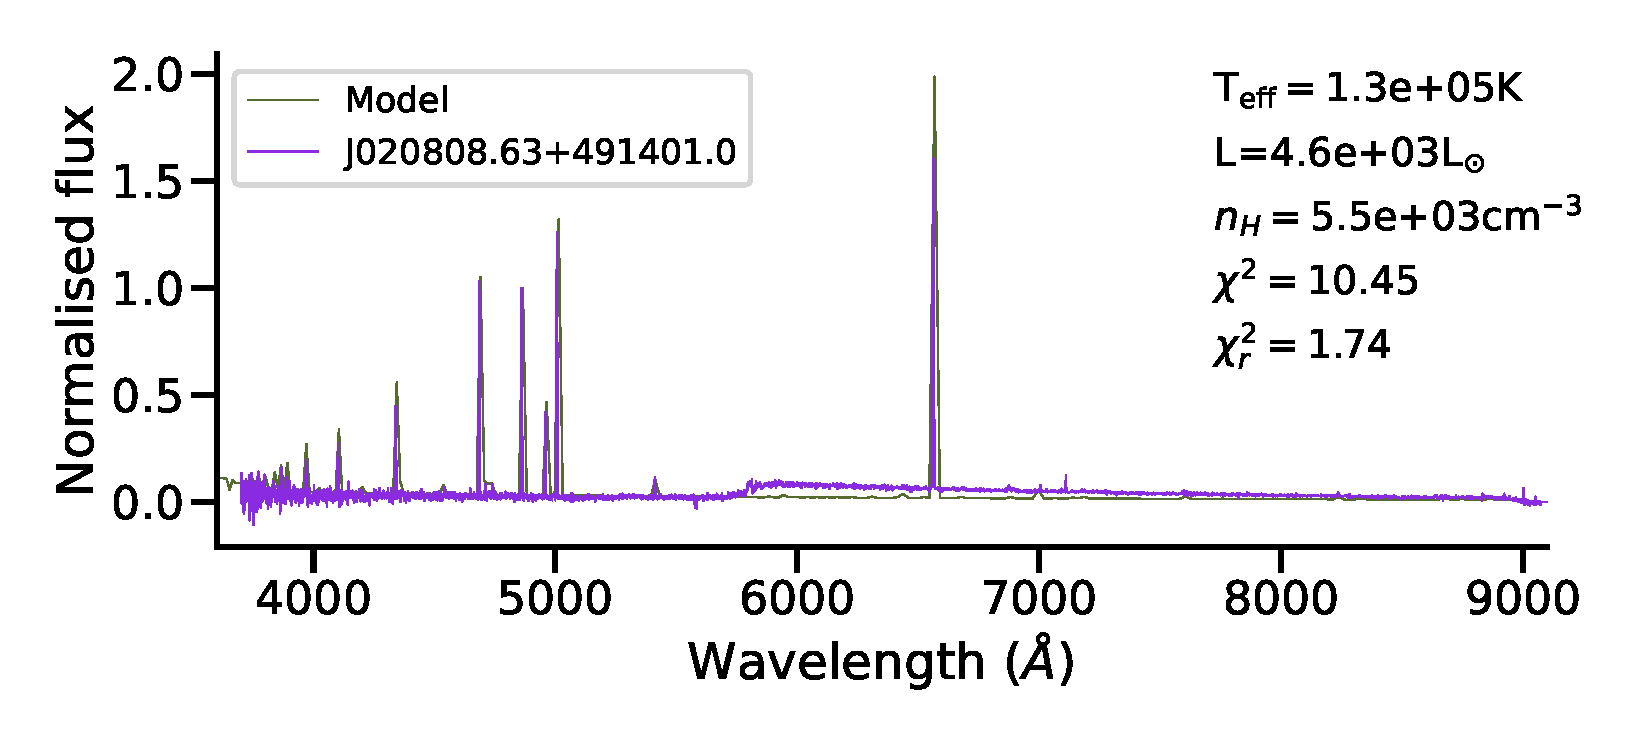
\includegraphics[width=0.24\linewidth, clip]{Figs/model_130000_37.25_3.74.pdf} \\
    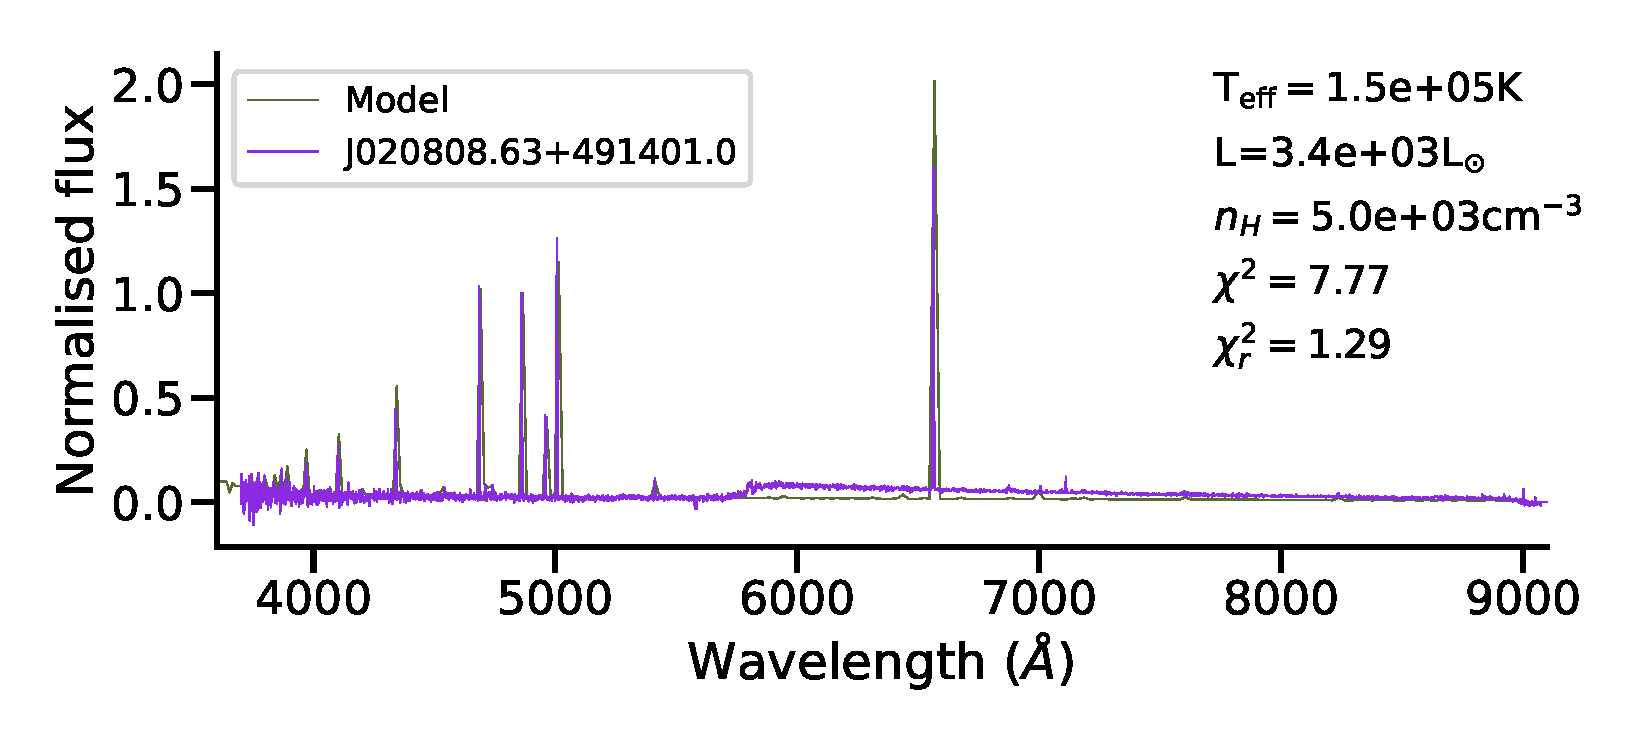
\includegraphics[width=0.24\linewidth, clip]{Figs/model_150000_37.12_3.70.pdf} & 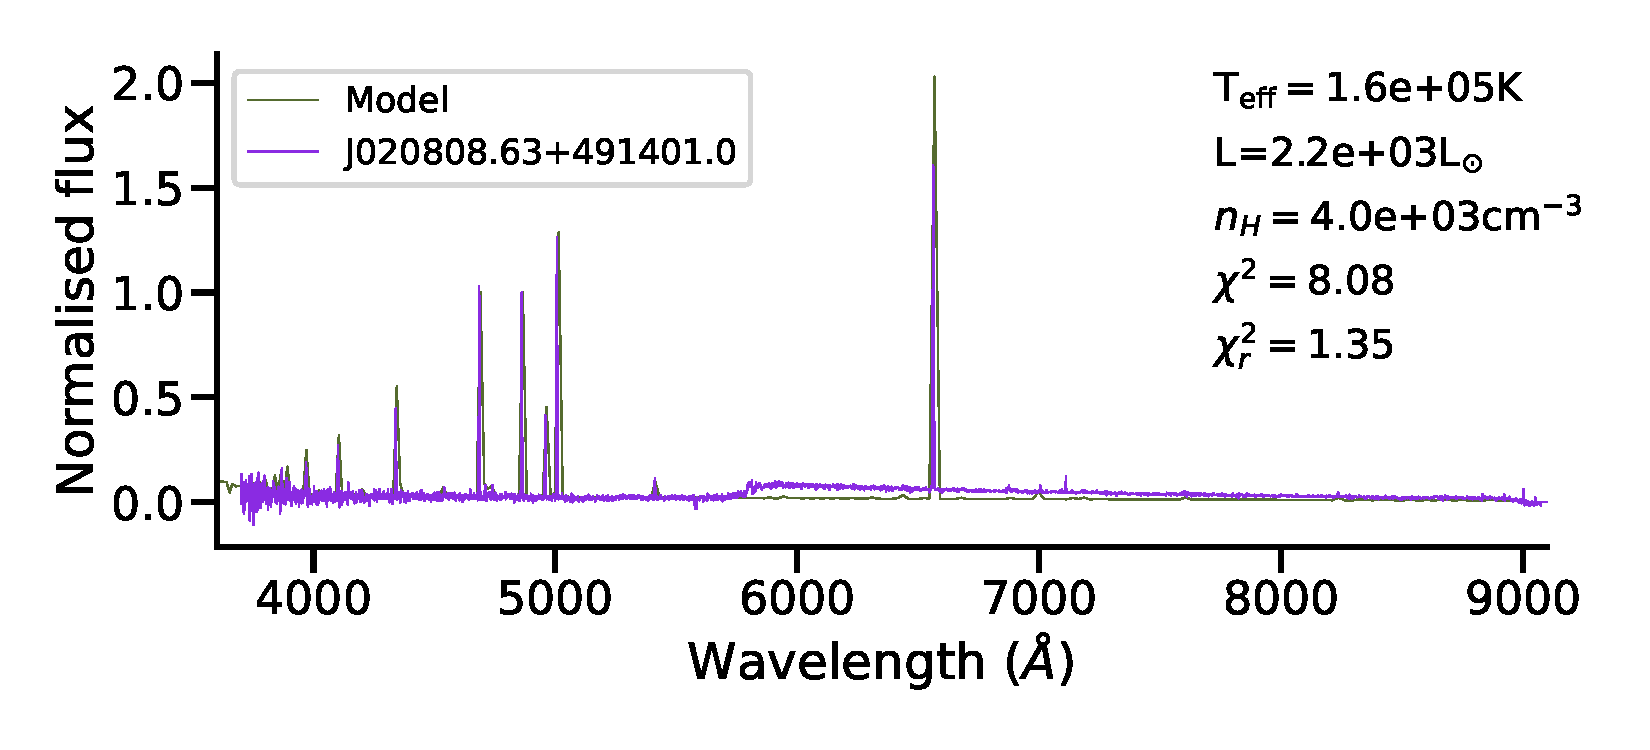
\includegraphics[width=0.24\linewidth, clip]{Figs/model_160000_36.93_3.60.pdf} & 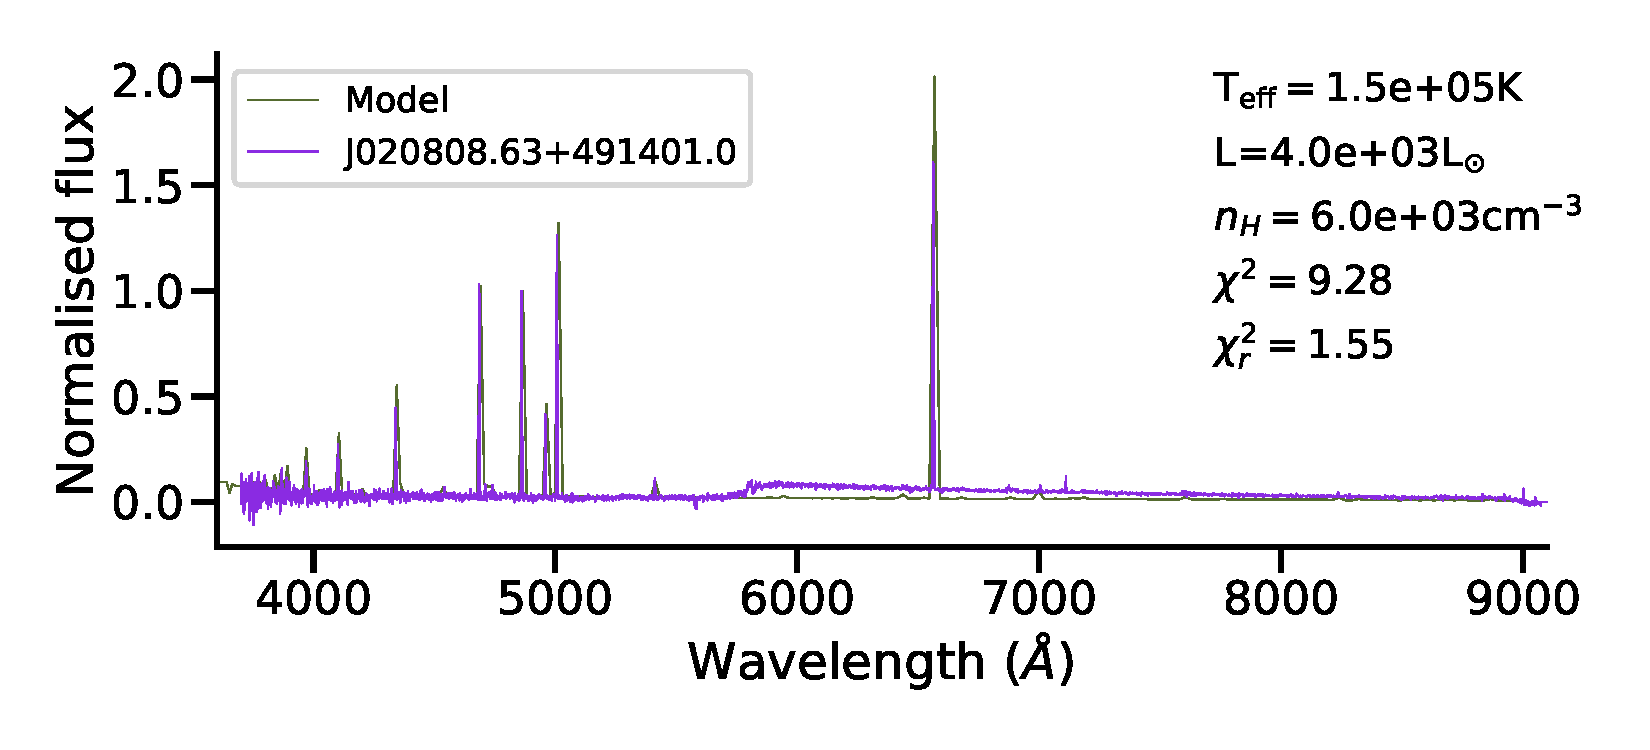
\includegraphics[width=0.24\linewidth, clip]{Figs/model_150000_37.19_3.78.pdf} & 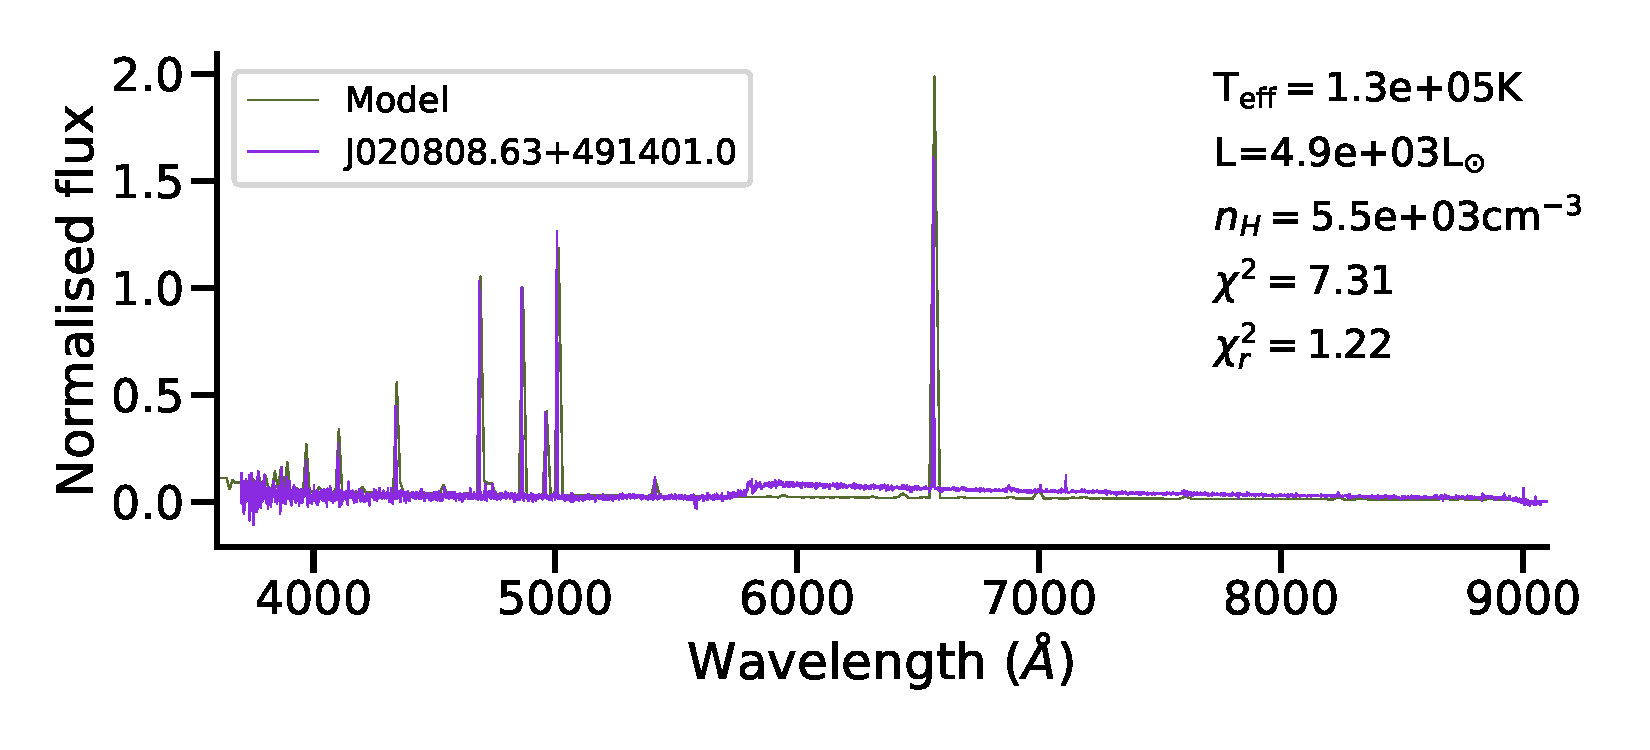
\includegraphics[width=0.24\linewidth, clip]{Figs/model_130000_37.27_3.74.pdf} \\
    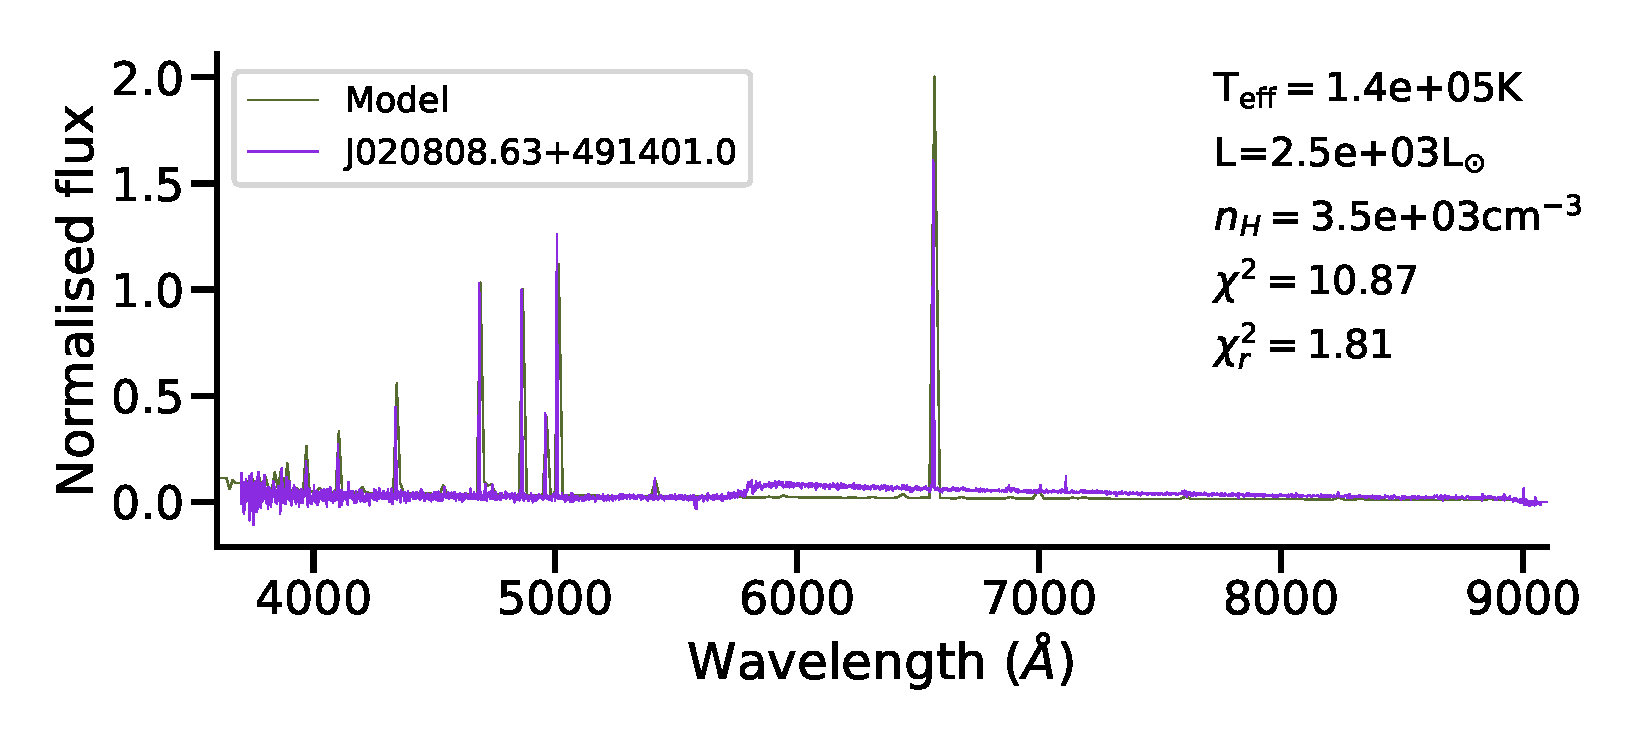
\includegraphics[width=0.24\linewidth, clip]{Figs/model_140000_36.98_3.54.pdf} & 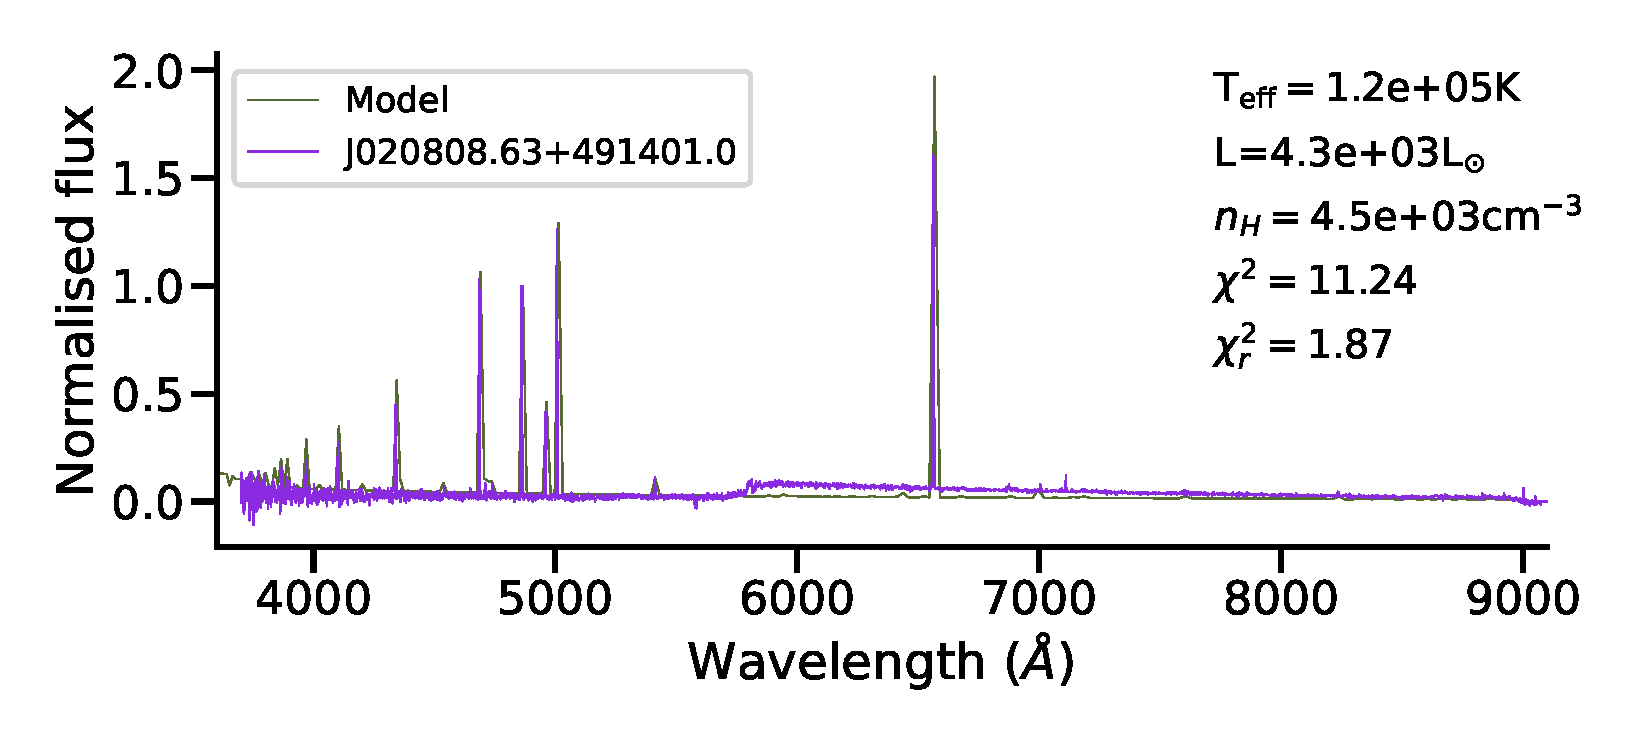
\includegraphics[width=0.24\linewidth, clip]{Figs/model_120000_37.22_3.65.pdf} & 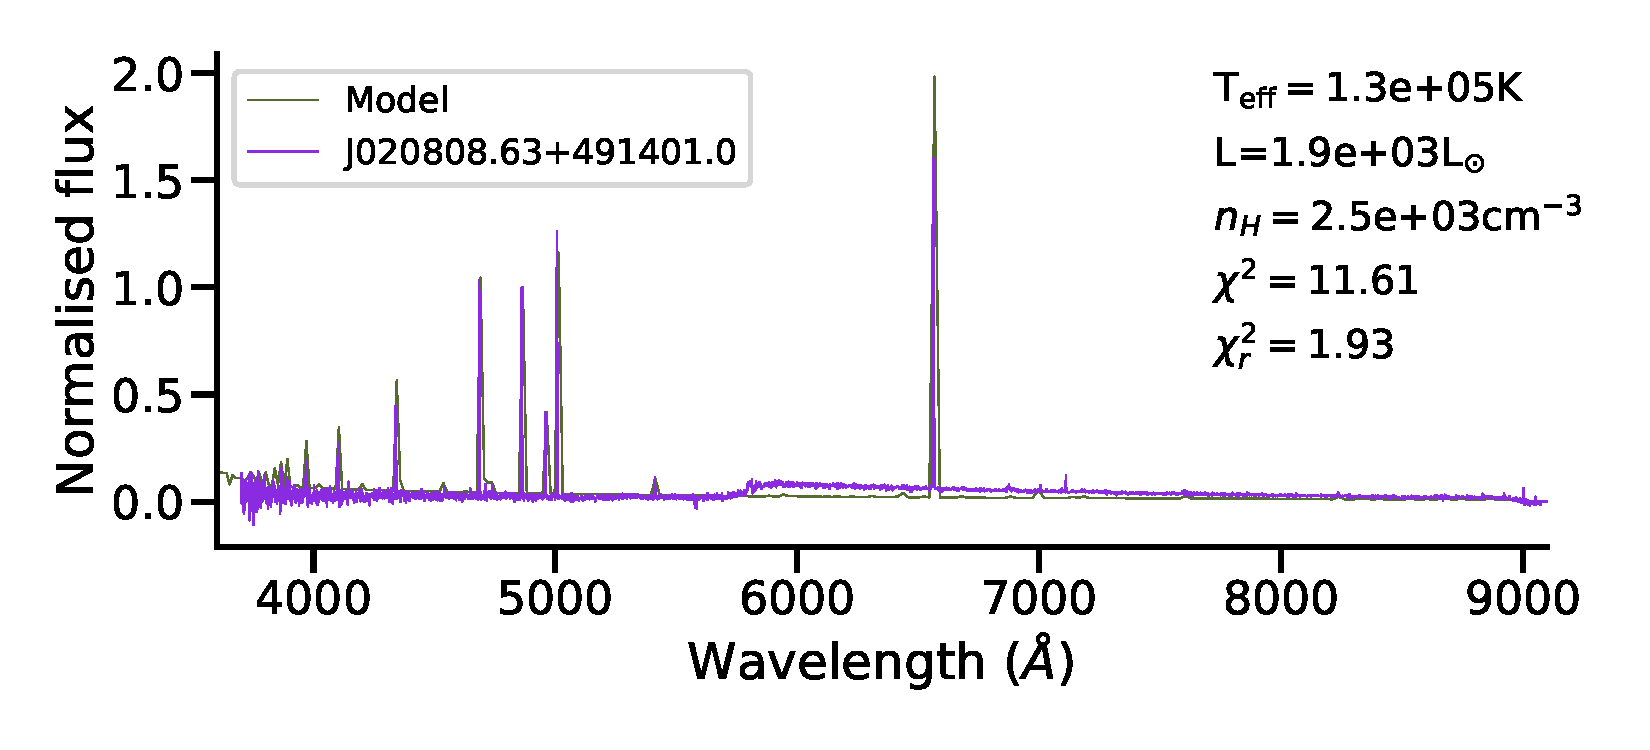
\includegraphics[width=0.24\linewidth, clip]{Figs/model_130000_36.86_3.40.pdf} & 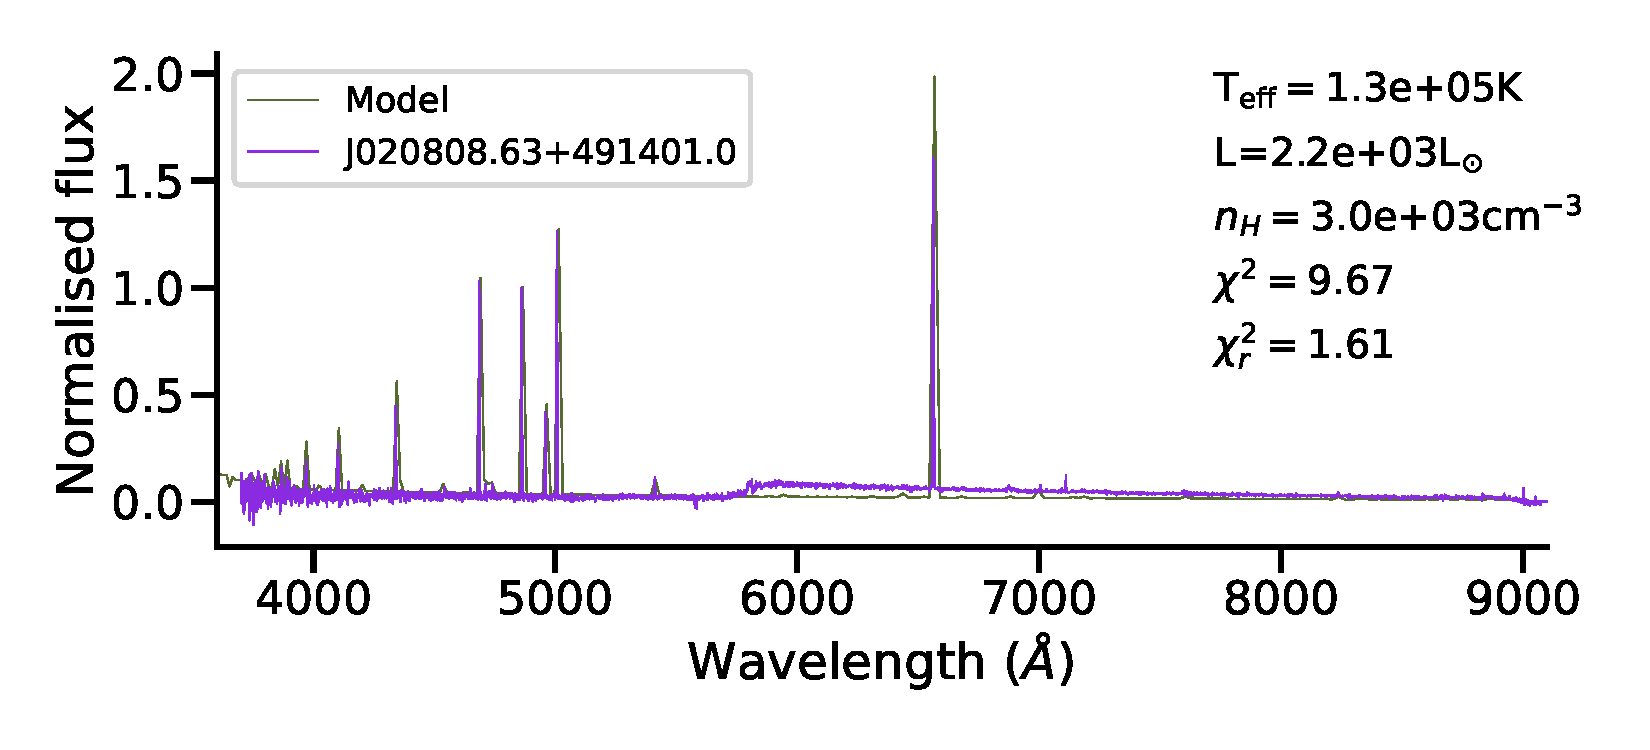
\includegraphics[width=0.24\linewidth, clip]{Figs/model_130000_36.93_3.48.pdf} \\
    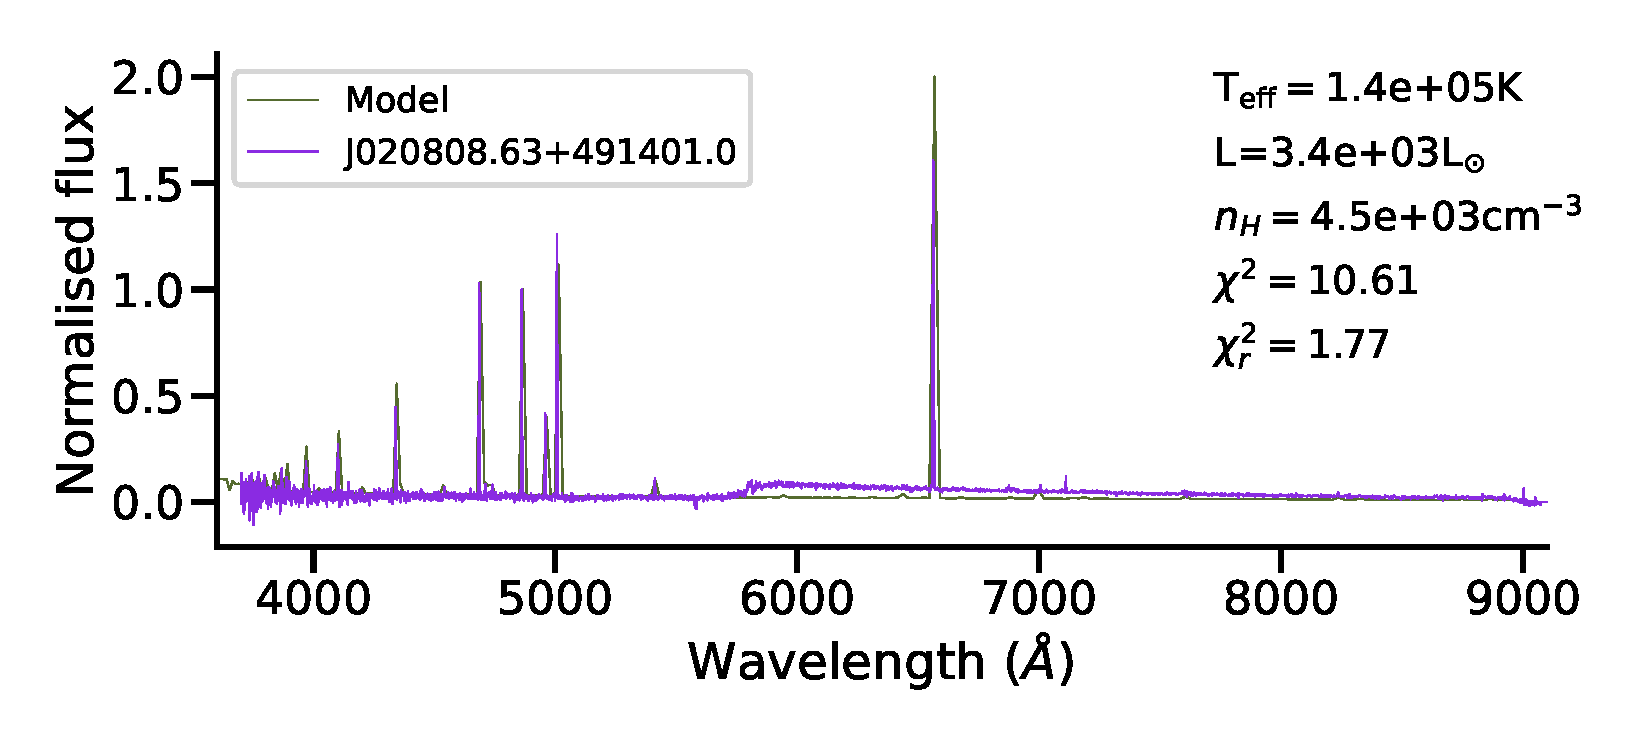
\includegraphics[width=0.24\linewidth, clip]{Figs/model_140000_37.12_3.65.pdf} & 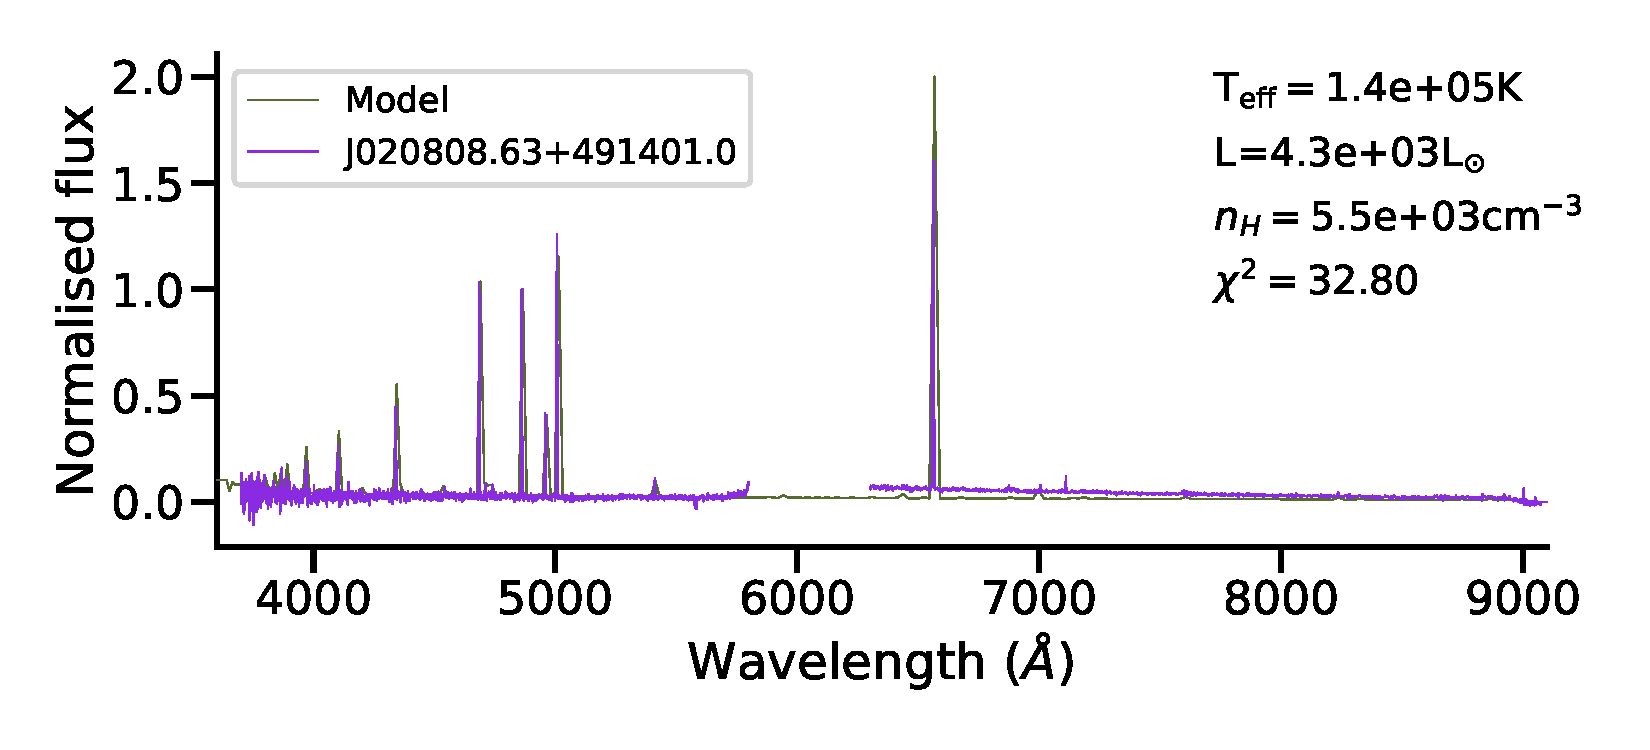
\includegraphics[width=0.24\linewidth, clip]{Figs/model_140000_37.22_3.74.pdf} & 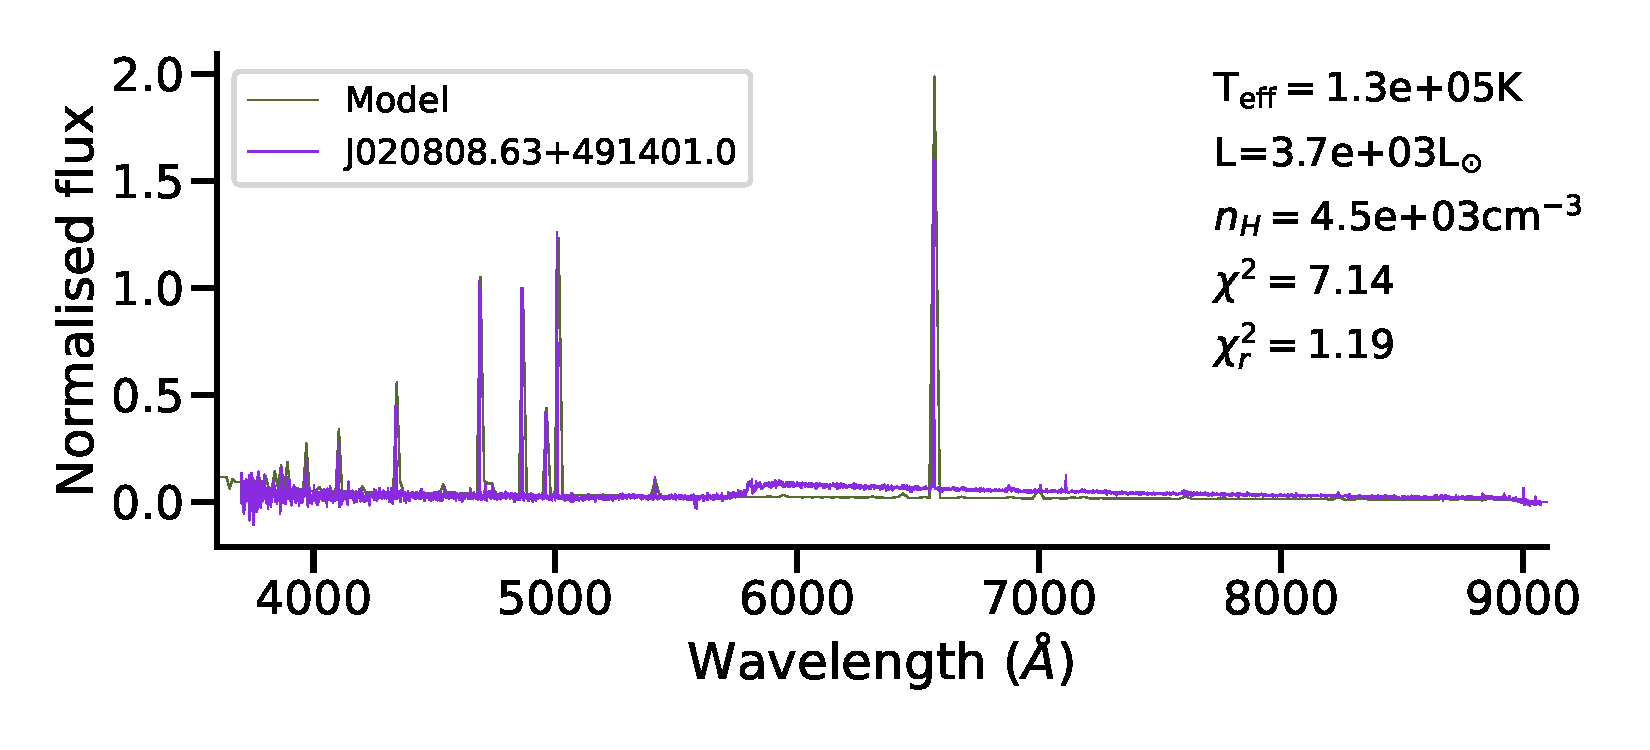
\includegraphics[width=0.24\linewidth, clip]{Figs/model_130000_37.15_3.65.pdf} & 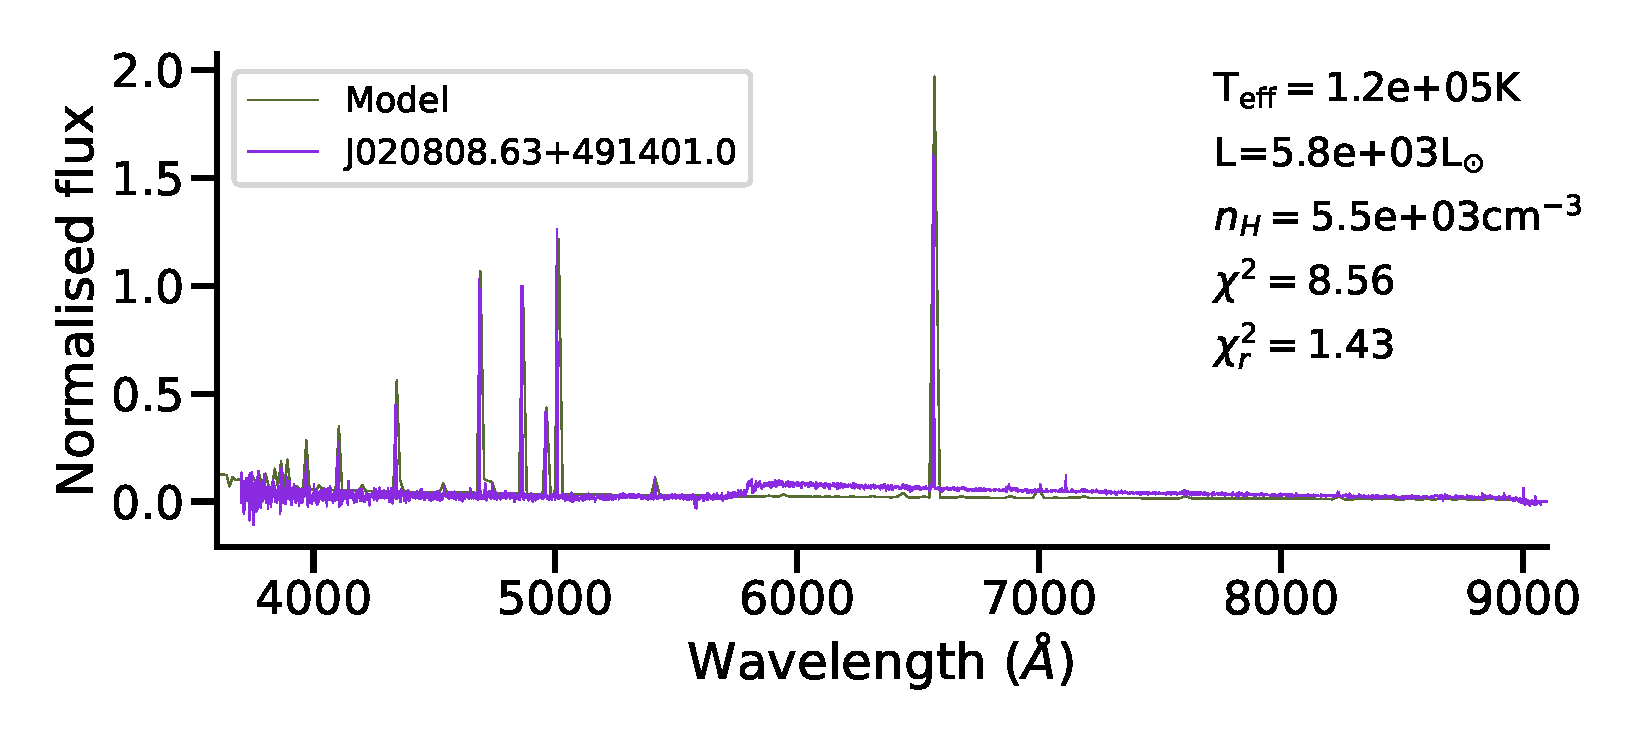
\includegraphics[width=0.24\linewidth, clip]{Figs/model_120000_37.35_3.74.pdf} \\
    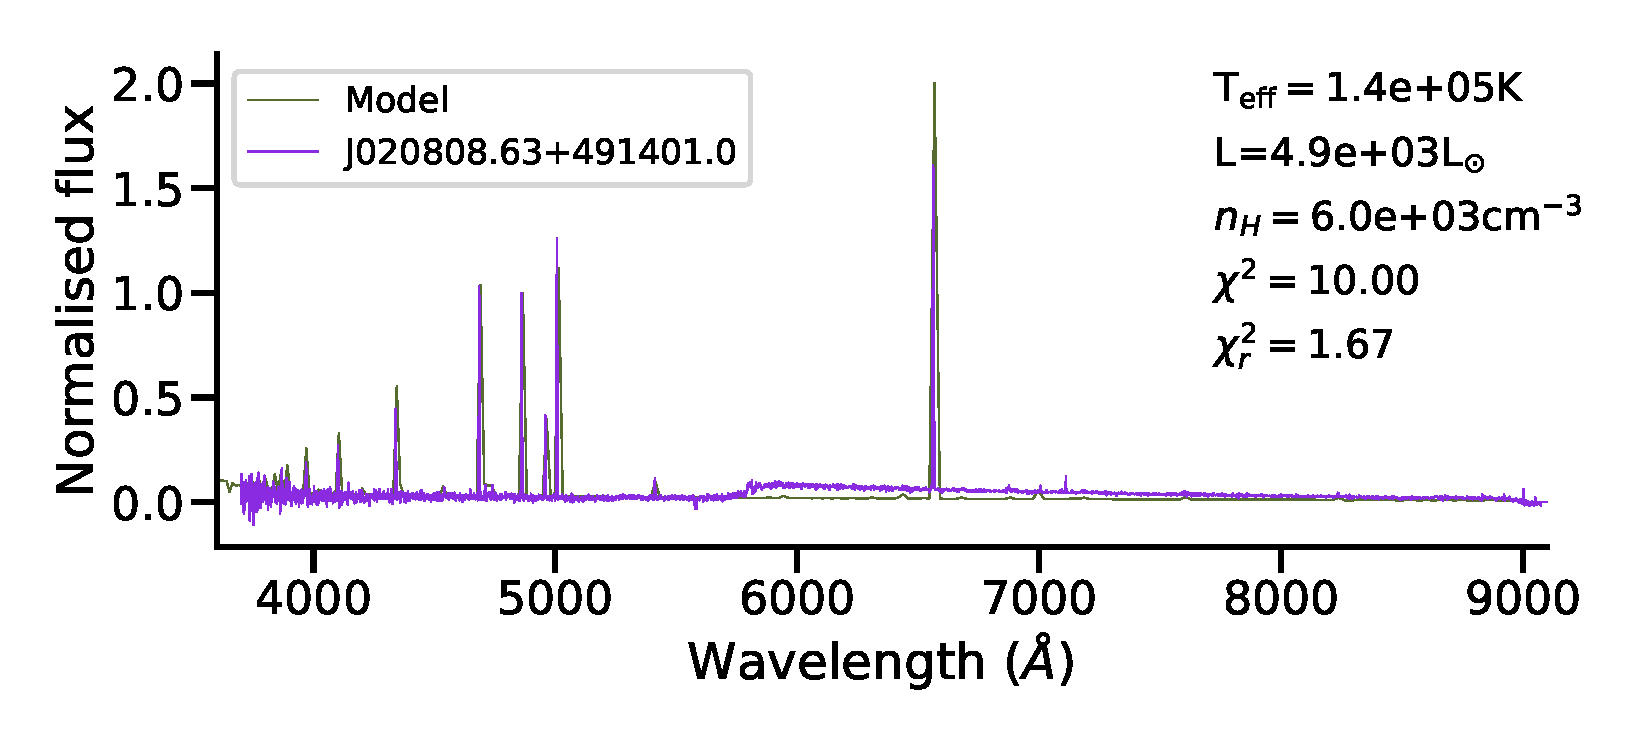
\includegraphics[width=0.24\linewidth, clip]{Figs/model_140000_37.27_3.78.pdf} & 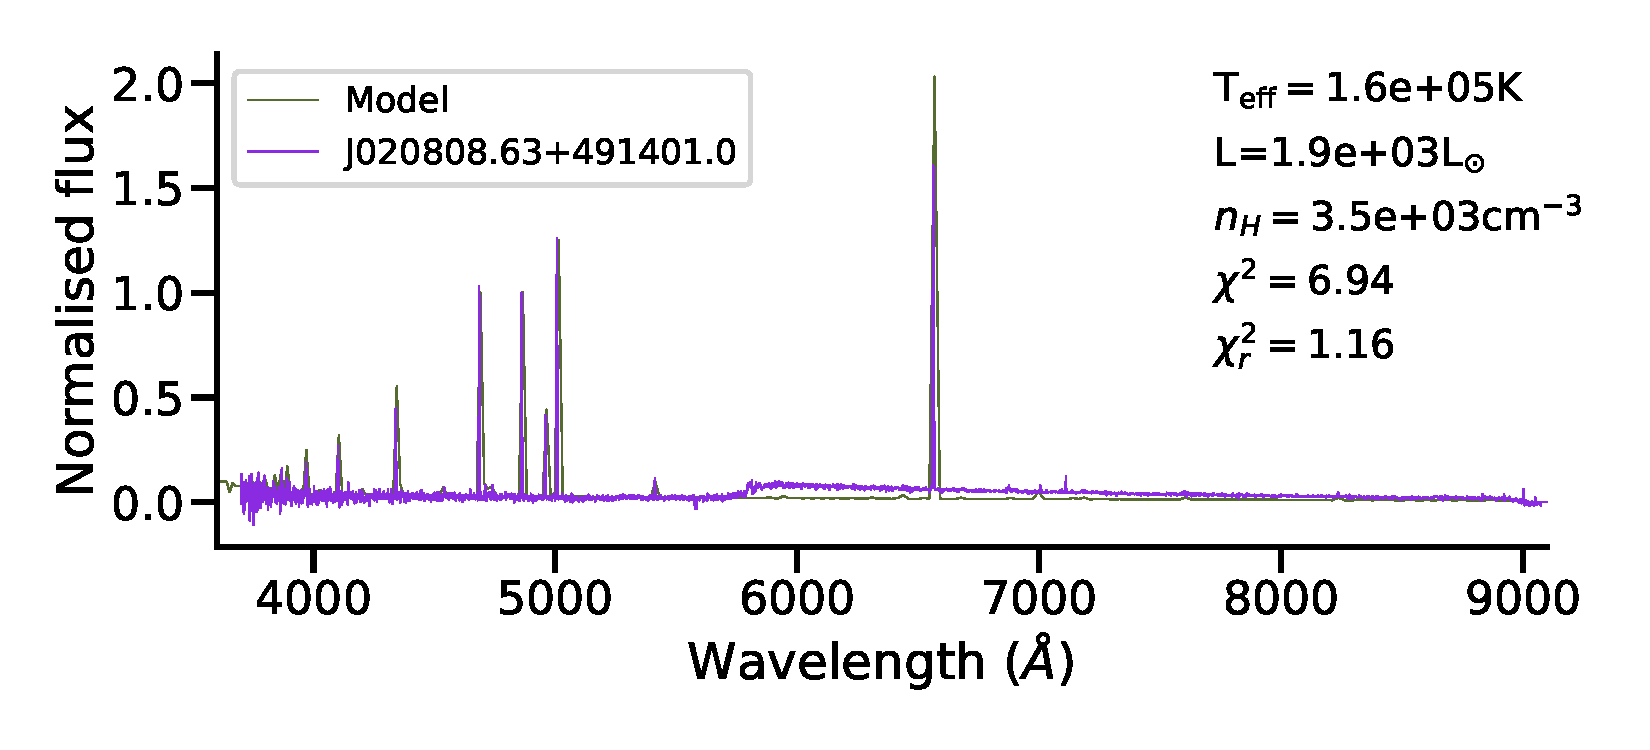
\includegraphics[width=0.24\linewidth, clip]{Figs/model_160000_36.86_3.54.pdf} & 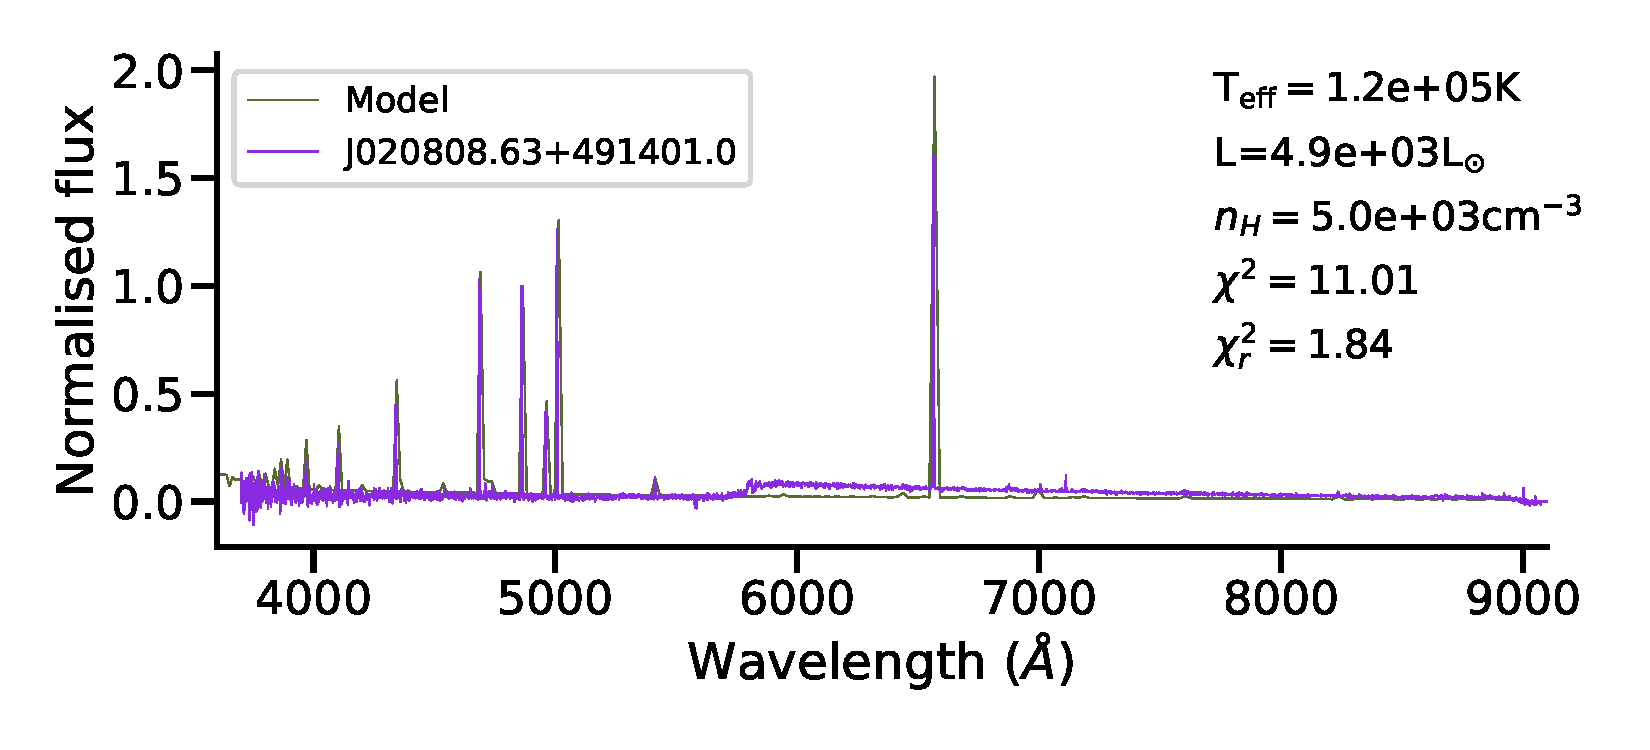
\includegraphics[width=0.24\linewidth, clip]{Figs/model_120000_37.27_3.70.pdf} & 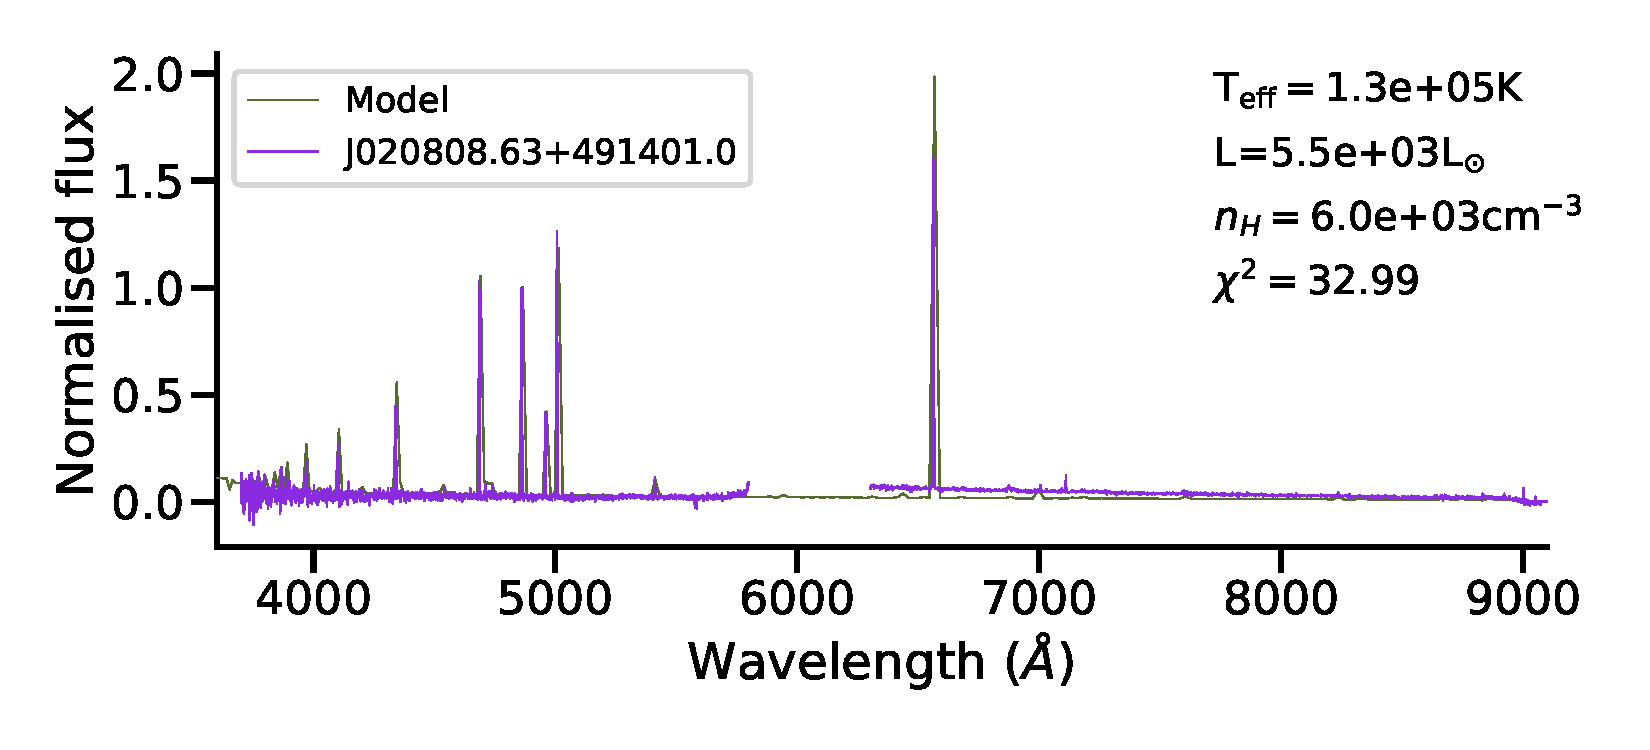
\includegraphics[width=0.24\linewidth, clip]{Figs/model_130000_37.32_3.78.pdf} \\
    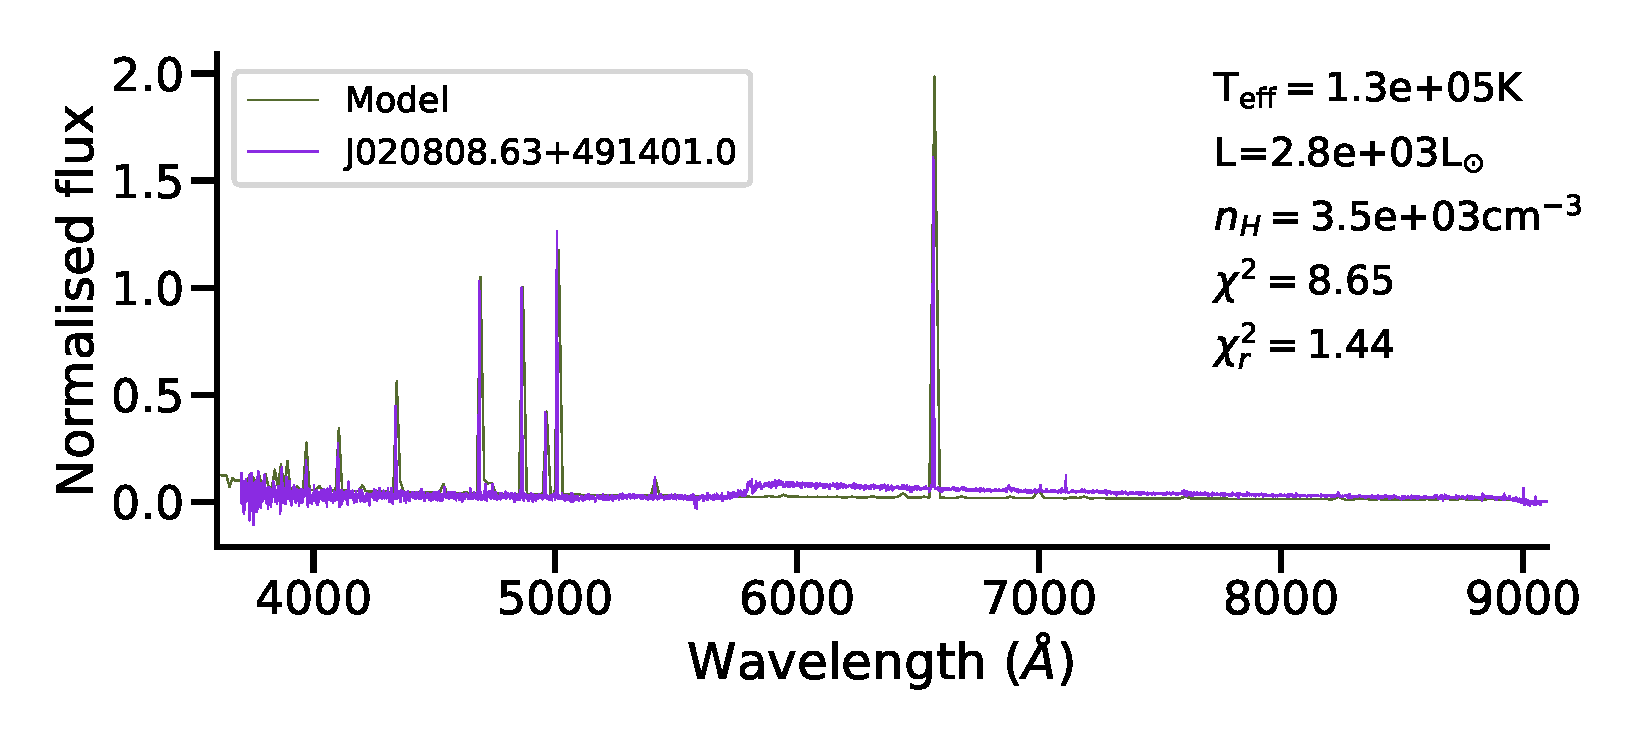
\includegraphics[width=0.24\linewidth, clip]{Figs/model_130000_37.03_3.54.pdf} & 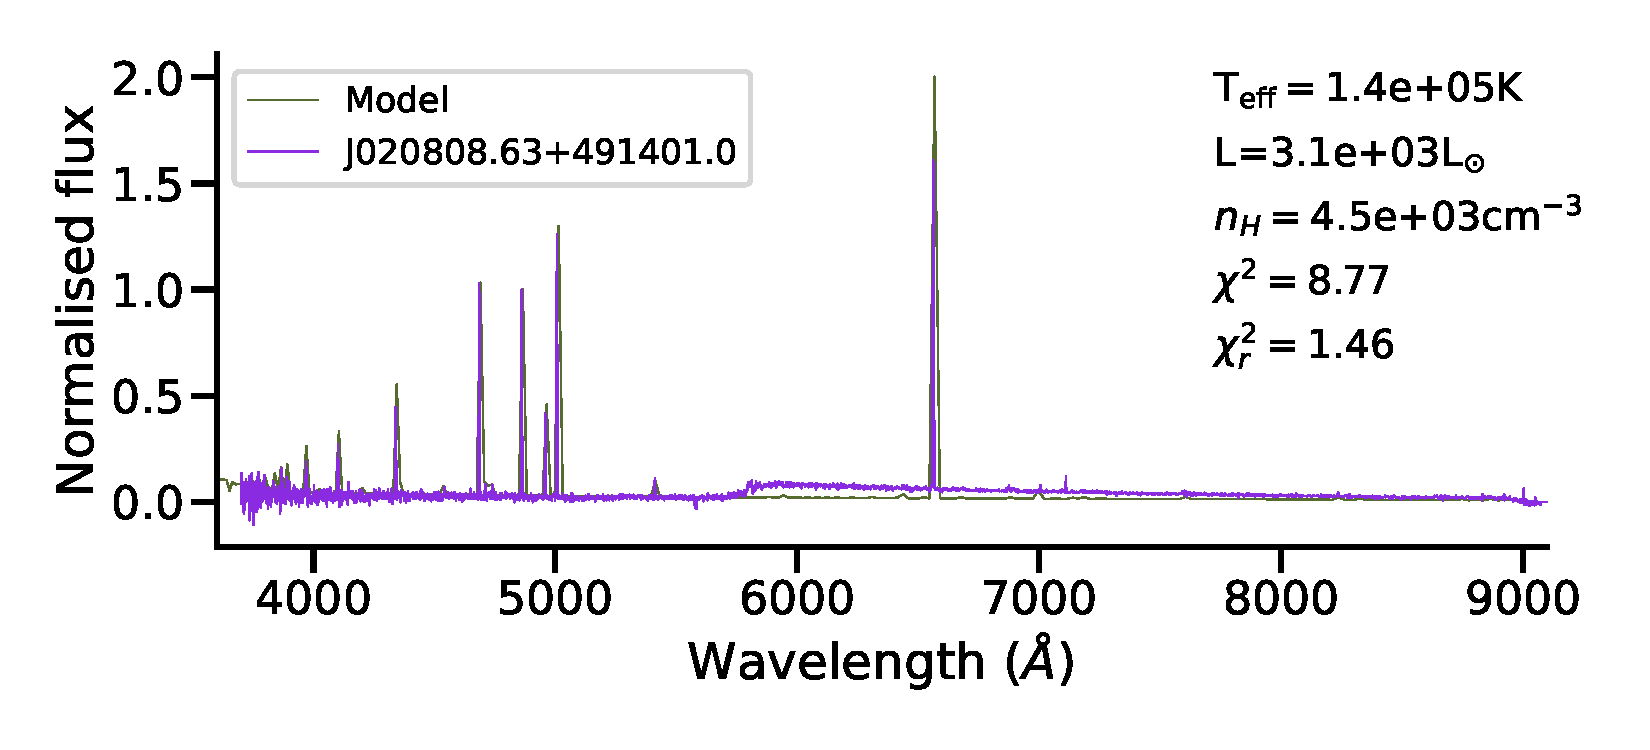
\includegraphics[width=0.24\linewidth, clip]{Figs/model_140000_37.08_3.65.pdf} & 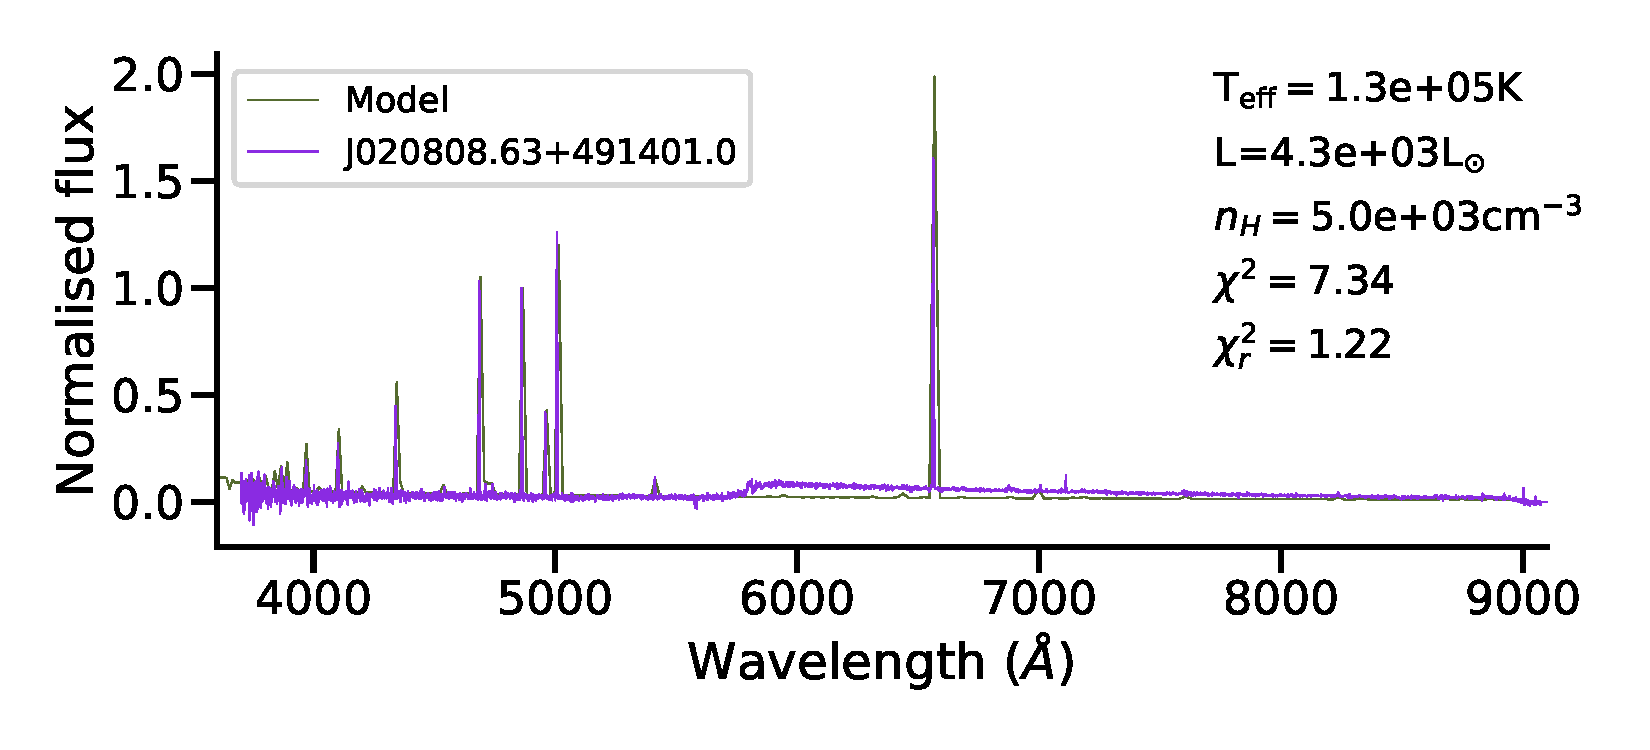
\includegraphics[width=0.24\linewidth, clip]{Figs/model_130000_37.22_3.70.pdf} & 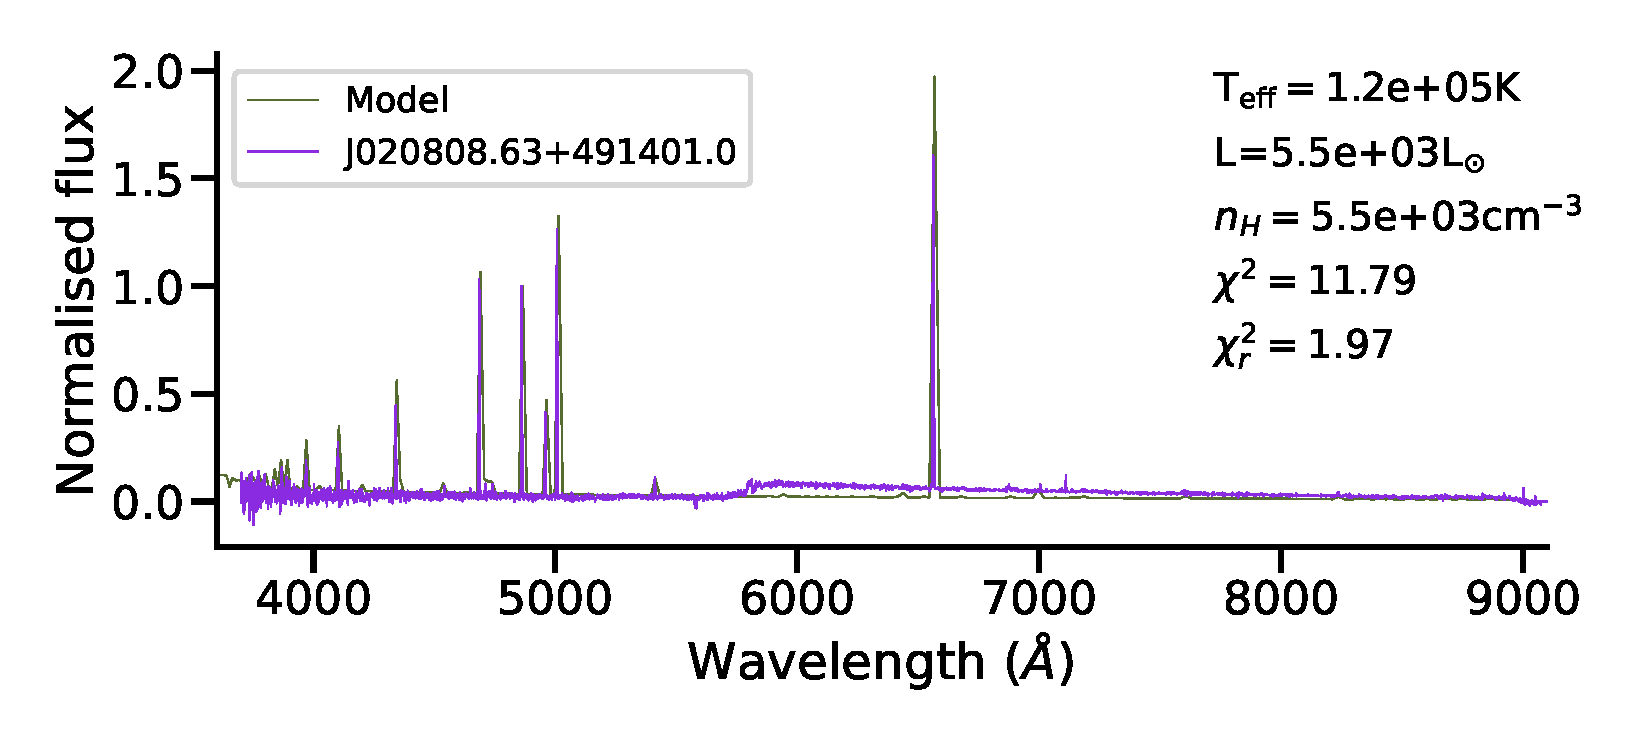
\includegraphics[width=0.24\linewidth, clip]{Figs/model_120000_37.32_3.74.pdf} \\
    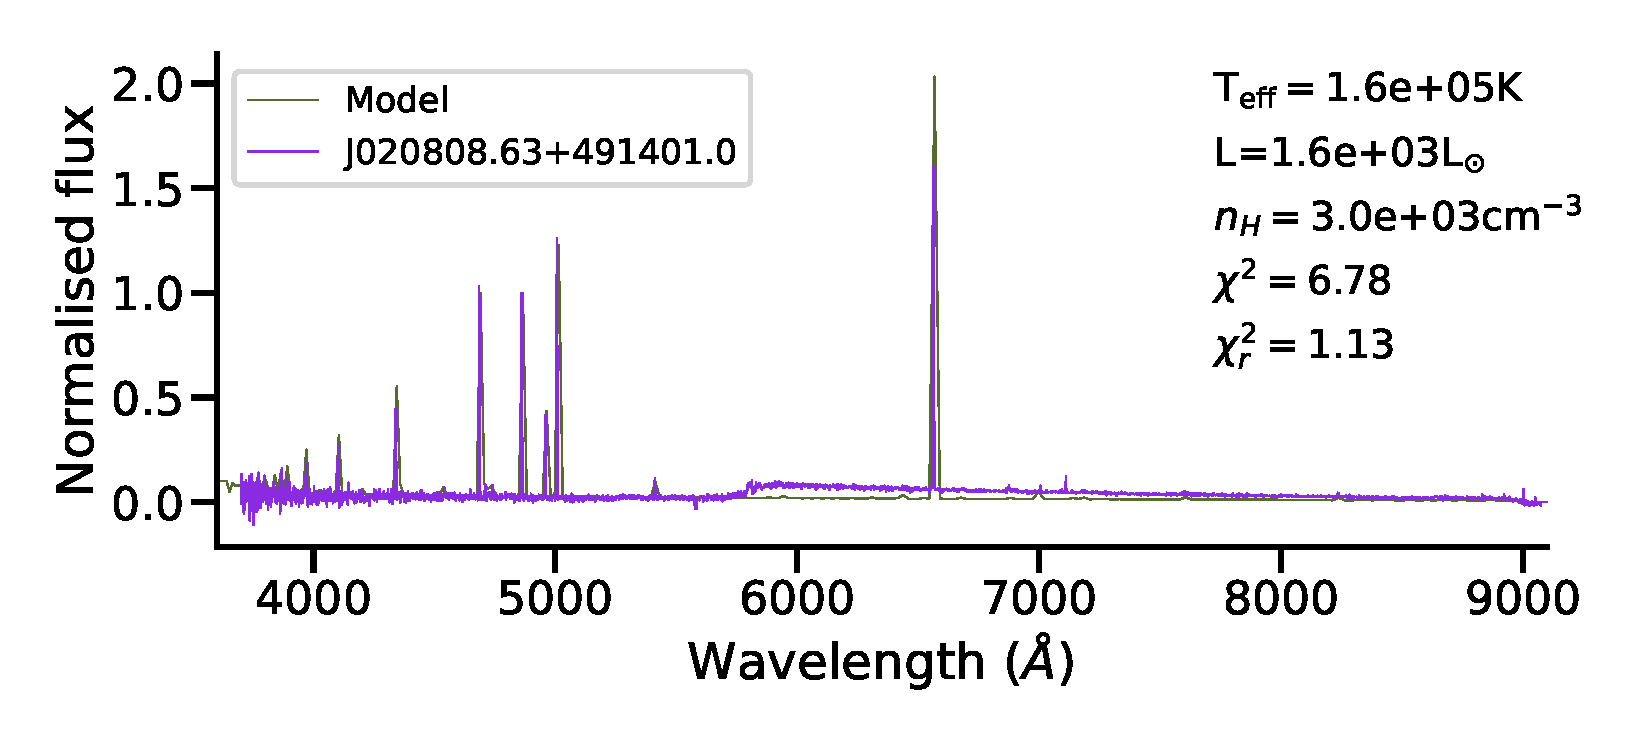
\includegraphics[width=0.24\linewidth, clip]{Figs/model_160000_36.79_3.48.pdf} & 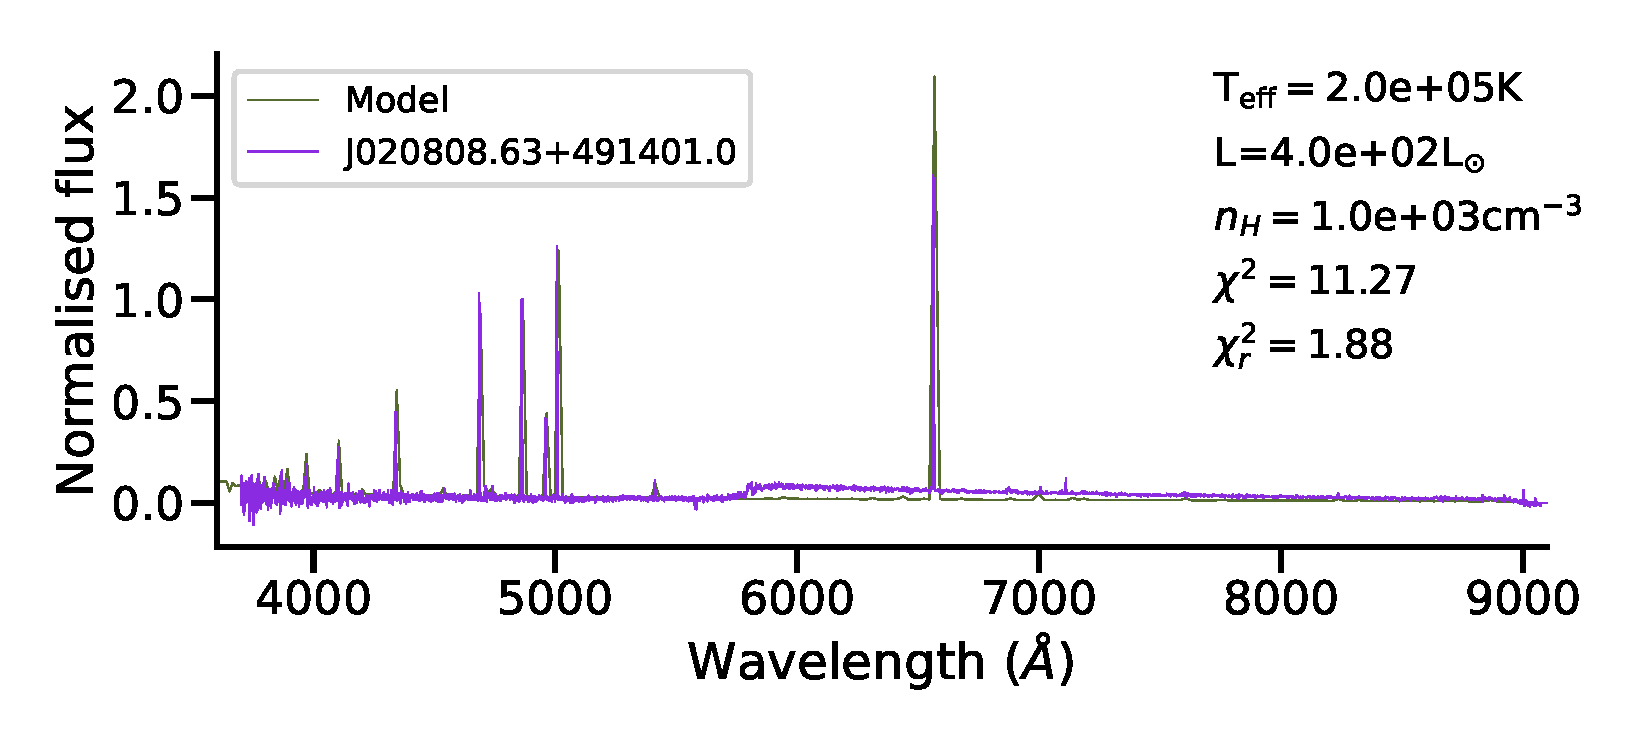
\includegraphics[width=0.24\linewidth, clip]{Figs/model_200000_36.19_3.00.pdf} & \includegraphics[width=0.24\linewidth, clip]{Figs/model_130000_37.12_3.60.pdf} & \includegraphics[width=0.24\linewidth, clip]{Figs/model_150000_37.03_3.65.pdf} \\
    \includegraphics[width=0.24\linewidth, clip]{Figs/model_120000_37.39_3.78.pdf} & \includegraphics[width=0.24\linewidth, clip]{Figs/model_170000_36.58_3.30.pdf} & \includegraphics[width=0.24\linewidth, clip]{Figs/model_130000_37.08_3.60.pdf} & \includegraphics[width=0.24\linewidth, clip]{Figs/model_170000_36.43_3.18.pdf} \\
    \includegraphics[width=0.24\linewidth, clip]{Figs/model_150000_37.22_3.78.pdf} & \includegraphics[width=0.24\linewidth, clip]{Figs/model_170000_36.86_3.54.pdf} & \includegraphics[width=0.24\linewidth, clip]{Figs/model_160000_36.70_3.40.pdf} & \includegraphics[width=0.24\linewidth, clip]{Figs/model_120000_37.30_3.70.pdf} \\
    \includegraphics[width=0.24\linewidth, clip]{Figs/model_130000_37.30_3.78.pdf} & \includegraphics[width=0.24\linewidth, clip]{Figs/model_140000_37.03_3.60.pdf} & \includegraphics[width=0.24\linewidth, clip]{Figs/model_140000_36.70_3.30.pdf} & \includegraphics[width=0.24\linewidth, clip]{Figs/model_150000_36.93_3.54.pdf} \\
    \includegraphics[width=0.24\linewidth, clip]{Figs/model_140000_36.79_3.40.pdf} & \includegraphics[width=0.24\linewidth, clip]{Figs/model_140000_36.86_3.48.pdf} & \includegraphics[width=0.24\linewidth, clip]{Figs/model_140000_37.19_3.74.pdf} \\
  \end{tabular}
\end{table*}


%%%%%%%%%%%%%%%%%%%%%%%%%%%%%%%%%%%%%%%%%%%%%%%%%%


% Don't change these lines
\bsp	% typesetting comment
\label{lastpage}
\end{document}

% End of mnras_template.tex
